\documentclass[10pt,twocolumn,letterpaper]{article}
\usepackage[utf8]{inputenc}
\usepackage[spanish,es-nodecimaldot]{babel}
\usepackage{amsmath}
\usepackage{amsfonts}
\usepackage{amssymb}
\usepackage{graphicx}
\usepackage{booktabs}
\usepackage{hyperref}
\usepackage{geometry}
\usepackage{float}
\usepackage{placeins}
\usepackage[dvipsnames]{xcolor}
\usepackage{titlesec}
\usepackage{parskip} 
\usepackage{microtype}
\usepackage{caption}
\usepackage{subcaption}
\usepackage{tcolorbox} 
\raggedbottom        

\geometry{left=1.8cm,right=1.8cm,top=2.2cm,bottom=2.2cm}

% Directorios de búsqueda de imágenes
\graphicspath{
    {./}
    {04_Figuras/}
    {../04_Figuras/}
    {06_Entregables/Candidata_1_trainbr/}
    {../06_Entregables/Candidata_1_trainbr/}
    {06_Entregables/Candidata_2_trainlm/}
    {../06_Entregables/Candidata_2_trainlm/}
    {Imagenes/}
}

% Paleta de Colores
\definecolor{ColorTitulo}{RGB}{35, 75, 170}
\definecolor{ColorTituloG}{RGB}{20, 45, 120}
\definecolor{ColorSUBTitulo}{RGB}{0, 120, 200}
\definecolor{GrisTabla}{RGB}{245, 247, 250}

\titleformat{\section}{\normalfont\large\bfseries\color{ColorTitulo}}{\thesection}{1em}{}
\titleformat{\subsection}{\normalfont\normalsize\bfseries\color{ColorSUBTitulo}}{\thesubsection}{1em}{}
\titleformat{\subsubsection}{\normalfont\small\bfseries\color{ColorTituloG}}{\thesubsubsection}{1em}{}

% Título y Metadatos
\title{\vspace{-1.2cm}\Large \textcolor{ColorTituloG}{\textbf{Taller 3: Diseño y Poda Estructural de un Perceptrón Multicapa mediante Optimal Brain Surgeon (OBS) con Aproximación de la Matriz Hessiana por Productos Externos}}}
\author{
  \normalsize \textbf{Maria Yuliany Sepulveda Bello} - 20202005013 \quad \textbf{Martin Felipe Gil Quemba} - 20221005040\\
  \normalsize \texttt{mysepulvedab@udistrital.edu.co} \quad \texttt{mfgilq@udistrital.edu.co}\vspace{0.15cm}\\
  \normalsize Inteligencia Computacional II --- Profesor: Andrés Eduardo Gaona Barrera\\
  \normalsize Universidad Distrital Francisco José de Caldas
}
\date{}

\begin{document}

\twocolumn[{%
    \maketitle
    \begin{abstract}
      En este trabajo se presenta el diseño, evaluación comparativa multi-algoritmo y poda estructural destructiva de un Perceptrón Multicapa (MLP) con topología inicial \texttt{10-60-1} ($n = 721$ parámetros totales; $660$ pesos sinápticos y $61$ sesgos) aplicado a la clasificación binaria supervisada sobre el conjunto de datos (\texttt{datos\_taller3.mat}, $P_{\text{total}} = 1{,}600$ patrones de desarrollo y $P_{\text{test}} = 13{,}888$ patrones de prueba ciega). Con el propósito de no restringir el análisis a una única familia de optimización, evaluamos un benchmark exhaustivo de $6$ algoritmos de entrenamiento (\texttt{trainbr}, \texttt{trainbfg}, \texttt{trainscg}, \texttt{traincgp}, \texttt{trainrp}, \texttt{trainlm}) cruzados con $3$ configuraciones de activación (\texttt{Config A: tanh+sig}, \texttt{Config B: tanh+lin}, \texttt{Config C: sig+sig}) y múltiples escalas de regularización y semillas ($156$ redes entrenadas). Siguiendo la formulación clásica de Hassibi y Stork (1993), implementamos el algoritmo \textit{Optimal Brain Surgeon} (OBS) de forma 100\% analítica pura sin reentrenamiento, construyendo recursivamente la inversa de la matriz Hessiana $\mathbf{H}^{-1}$ por productos externos de sensibilidades y la identidad de Sherman-Morrison-Woodbury sobre las redes evaluadas, comprobando que más del $97.9\%$ de la energía de Frobenius de $\mathbf{H}$ reside fuera de su diagonal principal y que \textit{Optimal Brain Damage} (OBD) sobreestima la curvatura efectiva del complemento de Schur $1/[\mathbf{H}^{-1}]_{qq}$ entre $537\times$ y $8\,819\times$. Al aplicar la poda destructiva OBS analítica pura, coronamos como campeona oficial a la \textbf{Red \#1 (\texttt{trainbr}, \texttt{tanh+lin}, seed \texttt{2102})}, la cual tras podar $553$ sinapsis ($83.79\%$ de compresión), sintetiza una arquitectura compacta equivalente \texttt{10-20-1} con $107$ sinapsis activas y $20$ neuronas ocultas activas ($128$ parámetros totales), alcanzando un error de prueba interna hold-out de $\mathbf{14.17\%}$ ($\text{Exactitud}=85.83\%$, $\text{AUC}=0.9281$, $\text{IC}_{95\%}\text{ Wilson}=[10.32\%, 19.14\%]$), y un error estimado ajustado por prevalencia en \texttt{x\_test} de $\mathbf{16.30\%}$ ($\text{IC}_{95\%}\text{ Bootstrap}=[13.03\%, 19.96\%]$). Como aporte de valor diferencial, documentamos en detalle la segunda opción Hipercompacta (\textbf{Red \#2, \texttt{trainlm}, \texttt{sig+sig}, seed \texttt{3603}}), la cual cura el sobreajuste podando $573$ sinapsis ($86.82\%$ de compresión) hasta una red \texttt{10-17-1} con $87$ sinapsis y $17$ neuronas ocultas activas, logrando $E_{\text{val}} = 0.0614$, error de prueba de $15.83\%$ y error ajustado en \texttt{x\_test} de $16.09\%$.
        
        \vspace{0.25cm}
        \textbf{Palabras clave:} Perceptrón Multicapa, Optimal Brain Surgeon (OBS), Optimal Brain Damage (OBD), Regularización Bayesiana, Levenberg-Marquardt, Matriz Hessiana, Identidad de Sherman-Morrison-Woodbury, Poda Estructural.
    \end{abstract}
    \vspace{0.35cm}
}]

% =========================================================================
\section{Fundamento Teórico y Matemático}
% =========================================================================

El diseño de redes neuronales artificiales enfrenta un compromiso fundamental entre capacidad de aproximación y capacidad de generalización. Una red subdimensionada es incapaz de capturar fronteras de decisión altamente no lineales, mientras que una red sobredimensionada memoriza el ruido muestral y deteriora su desempeño fuera de muestra \cite{hassibi1993}. Los métodos destructivos o de poda (\textit{network pruning}) resuelven esta disyuntiva entrenando una arquitectura inicialmente sobreparametrizada hasta un mínimo local y eliminando quirúrgicamente las conexiones redundantes mediante información de curvatura de segundo orden.

\subsection{Arquitectura del Perceptrón Multicapa (10-60-1) y Empaquetamiento Lexicográfico}
Consideremos un Perceptrón Multicapa (\textit{Multilayer Perceptron}, MLP) hacia adelante de tres capas con topología inicial \texttt{10-60-1}, conformado por $d = 10$ variables de entrada $\mathbf{x}^{[k]} \in \mathbb{R}^{10}$, una capa oculta con $M = 60$ unidades de procesamiento y una única neurona de salida escalar $o^{[k]} \in \mathbb{R}$. Para el $k$-ésimo patrón de entrada ($k \in \{1, \dots, P\}$), la propagación hacia adelante (\textit{forward pass}) viene dada por:
\begin{equation}
\begin{aligned}
    \mathbf{z}_1^{[k]} &= \mathbf{W}_1 \mathbf{x}^{[k]} + \mathbf{b}_1, \\
    \mathbf{a}_1^{[k]} &= f_{\text{hid}}\!\left(\mathbf{z}_1^{[k]}\right)
\end{aligned}
\label{eq:forward_oculta}
\end{equation}
\begin{equation}
\begin{aligned}
    z_2^{[k]} &= \mathbf{W}_2 \mathbf{a}_1^{[k]} + b_2, \\
    o^{[k]} &= F\!\left(\mathbf{w}, \mathbf{x}^{[k]}\right) = f_{\text{out}}\!\left(z_2^{[k]}\right)
\end{aligned}
\label{eq:forward_salida}
\end{equation}
donde $\mathbf{W}_1 \in \mathbb{R}^{60 \times 10}$ contiene los $600$ pesos sinápticos de entrada a capa oculta ($u_{ji}$), $\mathbf{b}_1 \in \mathbb{R}^{60 \times 1}$ es el vector de sesgos ocultos, $\mathbf{W}_2 = \mathbf{v}^T \in \mathbb{R}^{1 \times 60}$ agrupa los $60$ pesos sinápticos de capa oculta a salida ($v_j$), y $b_2 \in \mathbb{R}$ es el sesgo de salida. Para operar matricialmente sobre el espacio completo de parámetros, ensamblamos todas las matrices en un único vector columna $\mathbf{w} \in \mathbb{R}^{n \times 1}$ con $n = 10(60) + 60 + 60(1) + 1 = 721$ parámetros ($660$ pesos sinápticos podables y $61$ sesgos) siguiendo un ordenamiento lexicográfico estricto por columnas (\textit{column-major}):
\begin{equation}
    \mathbf{w} = \begin{bmatrix} \operatorname{vec}(\mathbf{W}_1)_{1:600} \\ (\mathbf{b}_1)_{601:660} \\ \operatorname{vec}(\mathbf{W}_2)_{661:720} \\ (b_2)_{721} \end{bmatrix} \in \mathbb{R}^{721 \times 1}
    \label{eq:empaquetamiento_w}
\end{equation}

Siguiendo la formulación de Hassibi y Stork \cite{hassibi1993} (Ec.~7), el ajuste supervisado minimiza el Error Cuadrático Medio (\textit{MSE}) reescalado por $\frac{1}{2P}$:
\begin{equation}
    E(\mathbf{w}) = \frac{1}{2P}\sum_{k=1}^{P}\left(t^{[k]} - o^{[k]}\right)^2
    \label{eq:mse_obs}
\end{equation}
donde $t^{[k]} \in \{0, 1\}$ denota la etiqueta verdadera del patrón $k$ y la predicción binaria se obtiene aplicando el umbral canónico $\hat{y}^{[k]} = \mathbb{I}\!\left(o^{[k]} \ge 0.5\right)$.

\subsection{Regularización Bayesiana de MacKay vs. Optimización Gauss-Newton}
Para comprender por qué diferentes algoritmos de entrenamiento condicionan radicalmente la poda OBS posterior, analizamos dos paradigmas de optimización de segundo orden:
\begin{enumerate}
    \item \textbf{Regularización Bayesiana de MacKay (\texttt{trainbr}) \cite{mackay1992, foresee1997}:} Enmarca el aprendizaje en una jerarquía Bayesiana donde se minimiza la función objetivo regularizada $F(\mathbf{w}) = \beta E_D(\mathbf{w}) + \alpha_{\text{reg}} E_W(\mathbf{w})$, con $E_D = \sum_{k=1}^P (t^{[k]}-o^{[k]})^2$ y $E_W = \frac{1}{2}\|\mathbf{w}\|_2^2$. Los hiperparámetros $\alpha_{\text{reg}}$ y $\beta$ se actualizan dinámicamente en cada época maximizando la evidencia marginal:
    \begin{equation}
    \begin{aligned}
        \gamma_{\text{eff}} &= \sum_{i=1}^{n} \frac{\lambda_i}{\lambda_i + \alpha_{\text{reg}}/\beta}, \\
        \alpha_{\text{reg}}^{\text{nuevo}} &= \frac{\gamma_{\text{eff}}}{\|\mathbf{w}\|_2^2}, \quad \beta^{\text{nuevo}} = \frac{P - \gamma_{\text{eff}}}{2 E_D(\mathbf{w})}
    \end{aligned}
    \label{eq:mackay_evidence}
    \end{equation}
    donde $\lambda_i$ son los autovalores de la matriz Hessiana Gauss-Newton y $\gamma_{\text{eff}} \in [0, n]$ representa el \textbf{número efectivo de parámetros libres}. La Regularización Bayesiana amortigua automáticamente las direcciones de curvatura casi nula ($\lambda_i \ll \alpha_{\text{reg}}/\beta$), colapsando los pesos redundantes hacia valores muy pequeños ($|w_q| < 0.10$) y reduciendo la norma $\|\mathbf{w}\|_2$ sin destruir la capacidad predictiva.
    \item \textbf{Levenberg-Marquardt (\texttt{trainlm}) \cite{hagan1994}:} Resuelve directamente la ecuación normal Gauss-Newton amortiguada:
    \begin{equation}
        \mathbf{w}^{(t+1)} = \mathbf{w}^{(t)} - \left(\mathbf{J}^T\mathbf{J} + \mu_{\text{LM}}\mathbf{I}_n\right)^{-1}\mathbf{J}^T\mathbf{e}
        \label{eq:lm_step}
    \end{equation}
    Al carecer de una penalización Bayesiana intrínseca sobre la norma de los pesos, LM tiende a amplificar las magnitudes sinápticas en direcciones espurias del espacio de parámetros, alcanzando mínimos locales con sobreajuste cuando la red base está sobredimensionada.
\end{enumerate}

\subsection{Algoritmos Destructivos de Poda: Magnitud, Optimal Brain Damage (OBD) y Optimal Brain Surgeon (OBS)}
Sea $\mathbf{w}^*$ un vector de pesos entrenado hasta un mínimo local de la superficie de error sobre los datos de entrenamiento. Al aplicar una perturbación $\delta\mathbf{w}$ sobre el vector de parámetros, la expansión en serie de Taylor de segundo orden de la función de error alrededor de $\mathbf{w}^*$ se expresa como \cite{hassibi1993, lecun1990}:
\begin{equation}
    \delta E = \left(\frac{\partial E}{\partial \mathbf{w}}\right)^T \delta\mathbf{w} + \frac{1}{2}\delta\mathbf{w}^T \mathbf{H} \delta\mathbf{w} + \mathcal{O}\!\left(\|\delta\mathbf{w}\|^3\right)
    \label{eq:taylor_error}
\end{equation}
donde $\mathbf{H} \equiv \frac{\partial^2 E}{\partial \mathbf{w}^2} \in \mathbb{R}^{n \times n}$ es la matriz Hessiana de segundas derivadas. En un mínimo local verdadero el término lineal desaparece ($\nabla_{\mathbf{w}} E \approx \mathbf{0}$) y, despreciando los términos de orden superior $\mathcal{O}(\|\delta\mathbf{w}\|^3)$, el incremento del error queda gobernado puramente por la forma cuadrática $\delta E \approx \frac{1}{2}\delta\mathbf{w}^T \mathbf{H} \delta\mathbf{w}$.

Eliminar el $q$-ésimo peso sináptico equivale a imponer la restricción lineal exacta $w_q + \delta w_q = 0$, la cual se escribe vectorialmente usando el $q$-ésimo vector canónico unitario $\mathbf{e}_q \in \mathbb{R}^{n \times 1}$ como $\mathbf{e}_q^T \delta\mathbf{w} + w_q = 0$. Formulando el funcional Lagrangiano con multiplicador escalar $\eta \in \mathbb{R}$:
\begin{equation}
    \mathcal{L}(\delta\mathbf{w}, \eta) = \frac{1}{2}\delta\mathbf{w}^T \mathbf{H} \delta\mathbf{w} - \eta\left(\mathbf{e}_q^T \delta\mathbf{w} + w_q\right)
    \label{eq:lagrangiano_obs}
\end{equation}
e igualando a cero las derivadas respecto a $\delta\mathbf{w}$ y $\eta$, se obtienen las dos ecuaciones fundamentales de \textit{Optimal Brain Surgeon} (Hassibi \& Stork \cite{hassibi1993}, Ec.~5):
\begin{equation}
\begin{aligned}
    \delta\mathbf{w} &= -\frac{w_q}{[\mathbf{H}^{-1}]_{qq}}\mathbf{H}^{-1}\mathbf{e}_q, \\
    L_q^{\text{OBS}} &= \frac{w_q^2}{2[\mathbf{H}^{-1}]_{qq}}
\end{aligned}
\label{eq:obs_fundamental}
\end{equation}
donde $L_q^{\text{OBS}}$ es la \textbf{saliencia} del peso $q$ y cuantifica el incremento mínimo posible en el error de entrenamiento cuando se elimina $w_q$ y se reajustan simultáneamente los demás $n-1$ pesos activos mediante el vector quirúrgico $\delta\mathbf{w}$.

La superioridad matemática de OBS sobre los métodos previos se comprende mediante la partición por bloques de $\mathbf{H}$ y el \textbf{Complemento de Schur}: si reordenamos el peso $q$ en la primera posición de modo que $\mathbf{H}$ tenga diagonal $(H_{qq}, \mathbf{H}_{\text{resto}})$ y acoplamiento $\mathbf{h}_q$, el elemento diagonal de la inversa satisface:
\begin{equation}
    \frac{1}{[\mathbf{H}^{-1}]_{qq}} = H_{qq} - \mathbf{h}_q^T \mathbf{H}_{\text{resto}}^{-1}\mathbf{h}_q \le H_{qq}
    \label{eq:complemento_schur}
\end{equation}
Dado que $\mathbf{H}_{\text{resto}}^{-1}$ es semidefinida positiva, el término $\mathbf{h}_q^T \mathbf{H}_{\text{resto}}^{-1}\mathbf{h}_q \ge 0$ mide cuánto pueden compensar los pesos correlacionados la pérdida de $w_q$. Esto demuestra que OBS contiene como casos particulares degradados a:
\begin{itemize}
    \item \textbf{Poda por Magnitud ($\mathbf{H} \propto \mathbf{I}$):} Asume curvatura isotrópica constante. No reajusta los pesos restantes ($\delta\mathbf{w} = -w_q\mathbf{e}_q$) y ordena por $L_q^{\text{Mag}} \propto w_q^2$.
    \item \textbf{Optimal Brain Damage --- OBD ($\mathbf{H} \approx \operatorname{diag}(\mathbf{H})$) \cite{lecun1990}:} Desprecia todos los términos cruzados fuera de la diagonal ($\mathbf{h}_q = \mathbf{0}$), aproximando $[\mathbf{H}^{-1}]_{qq} \approx 1/H_{qq}$. En consecuencia, tampoco actualiza los demás pesos y calcula una saliencia sobreestimada $L_q^{\text{OBD}} = \frac{1}{2}H_{qq}w_q^2 \ge L_q^{\text{OBS}}$.
\end{itemize}
Por tanto, en toda red neuronal con entradas o activaciones correlacionadas se cumple estrictamente la jerarquía de incremento de error en un paso:
\begin{equation}
    \Delta E(\text{Magnitud}) \ge \Delta E(\text{OBD}) \ge \Delta E(\text{OBS})
    \label{eq:desigualdad_teorema}
\end{equation}

\subsection{Inversa de la Matriz Hessiana mediante Productos Externos y Recursión de Woodbury}
Diferenciando dos veces la función de costo (\ref{eq:mse_obs}) respecto a $\mathbf{w}$, la Hessiana se descompone como (Ec.~10 de \cite{hassibi1993}):
\begin{equation}
\begin{aligned}
    \mathbf{H} = \frac{1}{P}\sum_{k=1}^{P}\Bigg[&\left(\frac{\partial F(\mathbf{w},\mathbf{x}^{[k]})}{\partial \mathbf{w}}\right)\!\left(\frac{\partial F(\mathbf{w},\mathbf{x}^{[k]})}{\partial \mathbf{w}}\right)^T \\
    &- \left(t^{[k]} - o^{[k]}\right)\frac{\partial^2 F(\mathbf{w},\mathbf{x}^{[k]})}{\partial \mathbf{w}^2}\Bigg]
\end{aligned}
\label{eq:hessiana_exacta}
\end{equation}
Para una red entrenada cerca de un mínimo local donde los residuos $(t^{[k]} - o^{[k]})$ son pequeños o no correlacionados con la curvatura de segundo orden de la salida, el segundo término se desprecia (aproximación de Gauss-Newton \cite{hassibi1993, singh2020}). Definiendo el vector de sensibilidad de la salida respecto a los pesos para el patrón $k$ como $\mathbf{X}^{[k]} \equiv \frac{\partial F(\mathbf{w}, \mathbf{x}^{[k]})}{\partial \mathbf{w}} \in \mathbb{R}^{721 \times 1}$, la matriz Hessiana se reduce a una suma de productos externos de rango $1$:
\begin{equation}
    \mathbf{H} \approx \frac{1}{P}\sum_{k=1}^{P} \mathbf{X}^{[k]}\!\left(\mathbf{X}^{[k]}\right)^T = \frac{1}{P}\mathbf{X}_{\text{mat}}\mathbf{X}_{\text{mat}}^T
    \label{eq:hessiana_outer}
\end{equation}
Aplicando la regla de la cadena a las ecuaciones (\ref{eq:forward_oculta})--(\ref{eq:forward_salida}) (Ecs.~19--21 de Hassibi \& Stork \cite{hassibi1993}), las derivadas analíticas exactas de los cuatro bloques de $\mathbf{X}^{[k]}$ son:
\begin{equation}
\begin{aligned}
    \mathbf{X}^{[k]} &= \begin{bmatrix} \operatorname{vec}\!\left(\boldsymbol{\delta}_1^{[k]}\!\left(\mathbf{x}^{[k]}\right)^T\right)_{1:600} \\ \left(\boldsymbol{\delta}_1^{[k]}\right)_{601:660} \\ \left(\delta_{\text{out}}^{[k]}\,\mathbf{a}_1^{[k]}\right)_{661:720} \\ \left(\delta_{\text{out}}^{[k]}\right)_{721} \end{bmatrix}, \\[4pt]
    \delta_{\text{out}}^{[k]} &= f_{\text{out}}'\!\left(z_2^{[k]}\right), \\
    \boldsymbol{\delta}_1^{[k]} &= \delta_{\text{out}}^{[k]}\,\mathbf{v} \odot f_{\text{hid}}'\!\left(\mathbf{z}_1^{[k]}\right)
\end{aligned}
\label{eq:bloques_sensibilidad}
\end{equation}
donde $\odot$ denota el producto elemento a elemento de Hadamard.

Dado que cada término $\mathbf{X}^{[k]}(\mathbf{X}^{[k]})^T$ es una perturbación de rango $1$, la matriz inversa amortiguada $(\mathbf{H} + \alpha\mathbf{I})^{-1}$ puede calcularse directamente acumulando los patrones $m = 0, 1, \dots, P-1$ mediante la identidad de inversión matricial de \textbf{Sherman-Morrison-Woodbury} \cite{hassibi1993, kailath1980} (Ec.~17 del artículo base):
\begin{equation}
\begin{aligned}
    \mathbf{H}_{m+1}^{-1} &= \mathbf{H}_m^{-1} \\
    &\quad - \frac{\mathbf{H}_m^{-1}\mathbf{X}^{[m+1]}\!\left(\mathbf{X}^{[m+1]}\right)^T\mathbf{H}_m^{-1}}{P + \left(\mathbf{X}^{[m+1]}\right)^T\mathbf{H}_m^{-1}\mathbf{X}^{[m+1]}}, \\
    \mathbf{H}_0^{-1} &= \alpha^{-1}\mathbf{I}_n
\end{aligned}
\label{eq:woodbury_recursion}
\end{equation}
donde $\mathbf{H}_P^{-1} = (\mathbf{H} + \alpha\mathbf{I}_n)^{-1}$ y $\alpha \in [10^{-8}, 10^{-3}]$ es el parámetro de regularización espectral de Tikhonov. Una vez eliminado un peso $q^*$ en un paso de poda, la inversa restringida al subespacio restante se proyecta en $\mathcal{O}(n^2)$ operaciones mediante la eliminación de Gauss-Jordan / Schur:
\begin{equation}
    \mathbf{H}_{\text{nuevo}}^{-1} = \mathbf{H}^{-1} - \frac{\left(\mathbf{H}^{-1}\mathbf{e}_{q^*}\right)\!\left(\mathbf{H}^{-1}\mathbf{e}_{q^*}\right)^T}{[\mathbf{H}^{-1}]_{q^*q^*}}
    \label{eq:gauss_jordan_update}
\end{equation}

% =========================================================================
\section{Base de Datos y Estrategia de Partición}
% =========================================================================

\subsection{Caracterización Estadística de \texttt{datos\_taller3.mat}}
El archivo oficial \texttt{datos\_taller3.mat} contiene la matriz de entrenamiento \texttt{x\_train} $\in \mathbb{R}^{1600 \times 10}$, el vector de etiquetas binarias \texttt{y\_train} $\in \{0, 1\}^{1600 \times 1}$ con balance exacto $1:1$ de $800$ muestras de Clase~$0$ ($50.0\%$) y $800$ muestras de Clase~$1$ ($50.0\%$), y la matriz de evaluación ciega \texttt{x\_test} $\in \mathbb{R}^{13888 \times 10}$ conformada por $d = 10$ variables numéricas continuas anónimas ($x_1, \dots, x_{10}$).

\begin{table}[htbp]
\centering
\caption{Caracterización estadística, poder discriminante de Fisher ($J_i$), $\text{AUC}$ univariado y prueba de Kolmogorov-Smirnov ($KS$) en \texttt{datos\_taller3.mat}.}
\label{tab:eda_variables}
\vspace{0.1cm}
\resizebox{\columnwidth}{!}{%
\begin{tabular}{lccccccccc}
\toprule
\textbf{Var.} & \textbf{Mín Tr} & \textbf{Máx Tr} & $\boldsymbol{\mu_{C0}}$ & $\boldsymbol{\mu_{C1}}$ & $\boldsymbol{\sigma_{C0}}$ & $\boldsymbol{\sigma_{C1}}$ & \textbf{Fisher $\boldsymbol{J_i}$} & $\textbf{AUC}_i$ & $\boldsymbol{KS}_{\text{Tr-Te}}$ \\
\midrule
$x_1$  & $8.231$    & $305.096$ & $72.912$  & $43.658$  & $59.528$ & $24.937$ & $0.2055$ & $0.6205$ & $0.0341$ \\
$x_2$   & $0.000$    & $190.139$ & $29.891$  & $18.859$  & $28.316$ & $9.537$  & $0.1363$ & $0.5453$ & $0.0363$ \\
$x_3$    & $2.006$    & $4.649$   & $2.919$   & $2.796$   & $0.491$  & $0.463$  & $0.0328$ & $0.5740$ & $0.0405$ \\
$x_4$    & $0.021$    & $0.877$   & $0.369$   & $0.378$   & $0.195$  & $0.176$  & $0.0013$ & $0.5178$ & $0.0252$ \\
$x_5$   & $0.005$    & $0.637$   & $0.211$   & $0.214$   & $0.119$  & $0.107$  & $0.0005$ & $0.5161$ & $0.0224$ \\
$x_6$    & $-449.953$ & $473.065$ & $-16.784$ & $2.826$   & $84.607$ & $38.938$ & $0.0443$ & $0.5819$ & $0.0258$ \\
$x_7$  & $-284.704$ & $200.315$ & $-5.267$  & $17.028$  & $73.484$ & $33.798$ & $0.0760$ & $0.5740$ & $0.0285$ \\
$x_8$ & $-142.589$ & $122.462$ & $-0.619$  & $0.230$   & $30.587$ & $13.727$ & $0.0006$ & $0.5011$ & $0.0160$ \\
$x_9$   & $0.000$    & $89.954$  & $43.478$  & $18.850$  & $26.044$ & $21.377$ & $\mathbf{0.5343}$ & $\mathbf{0.7797}$ & $0.0386$ \\
$x_{10}$ & $5.700$    & $430.119$ & $197.284$ & $190.875$ & $82.474$ & $70.450$ & $0.0035$ & $0.5210$ & $0.0186$ \\
\bottomrule
\end{tabular}%
}
\end{table}

\begin{figure}[H]
    \centering
    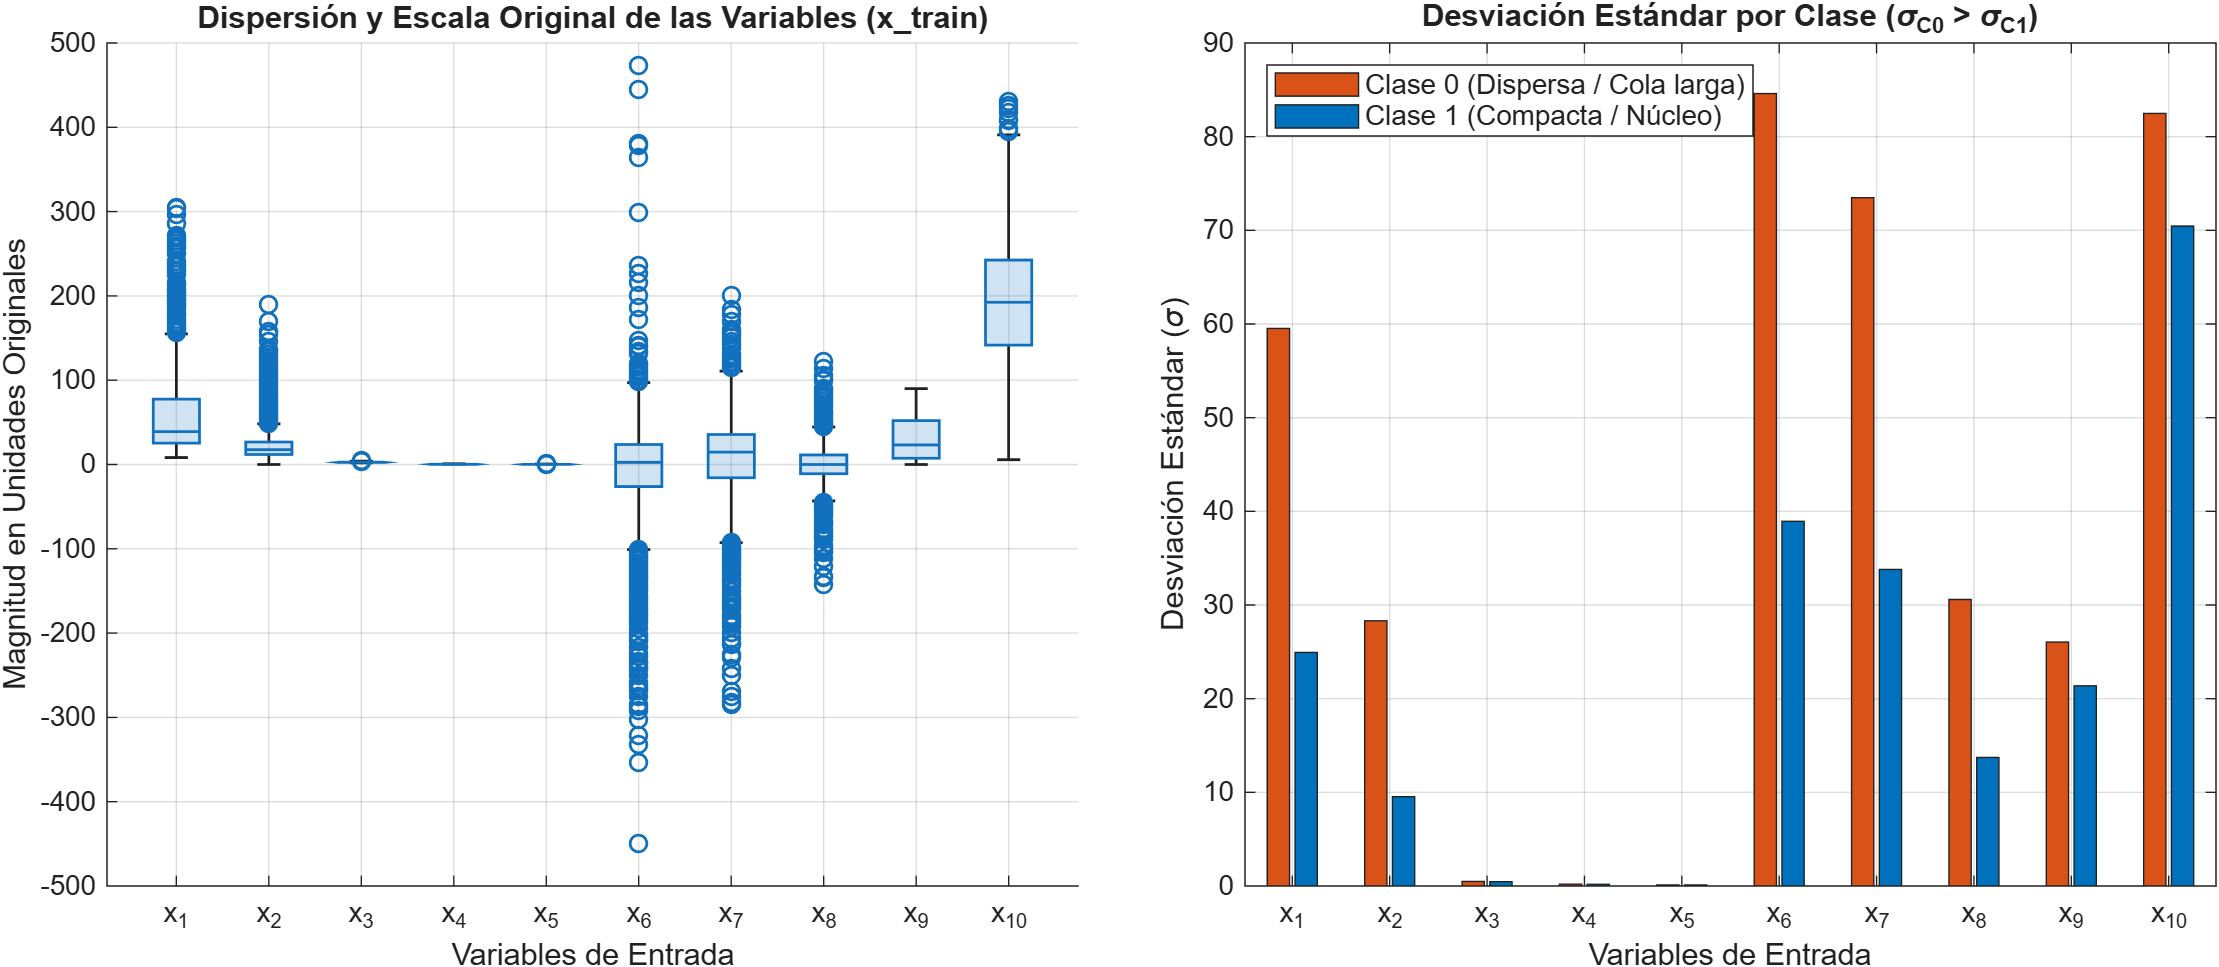
\includegraphics[width=1\columnwidth]{fig1_escalas_y_dispersion.png}
    \caption{Dispersión en unidades originales de \texttt{x\_train} (izquierda) y contraste de desviaciones estándar por clase $\sigma_{C0} > \sigma_{C1}$ (derecha).}
    \label{fig:eda_escalas}
\end{figure}

\begin{figure}[H]
    \centering
    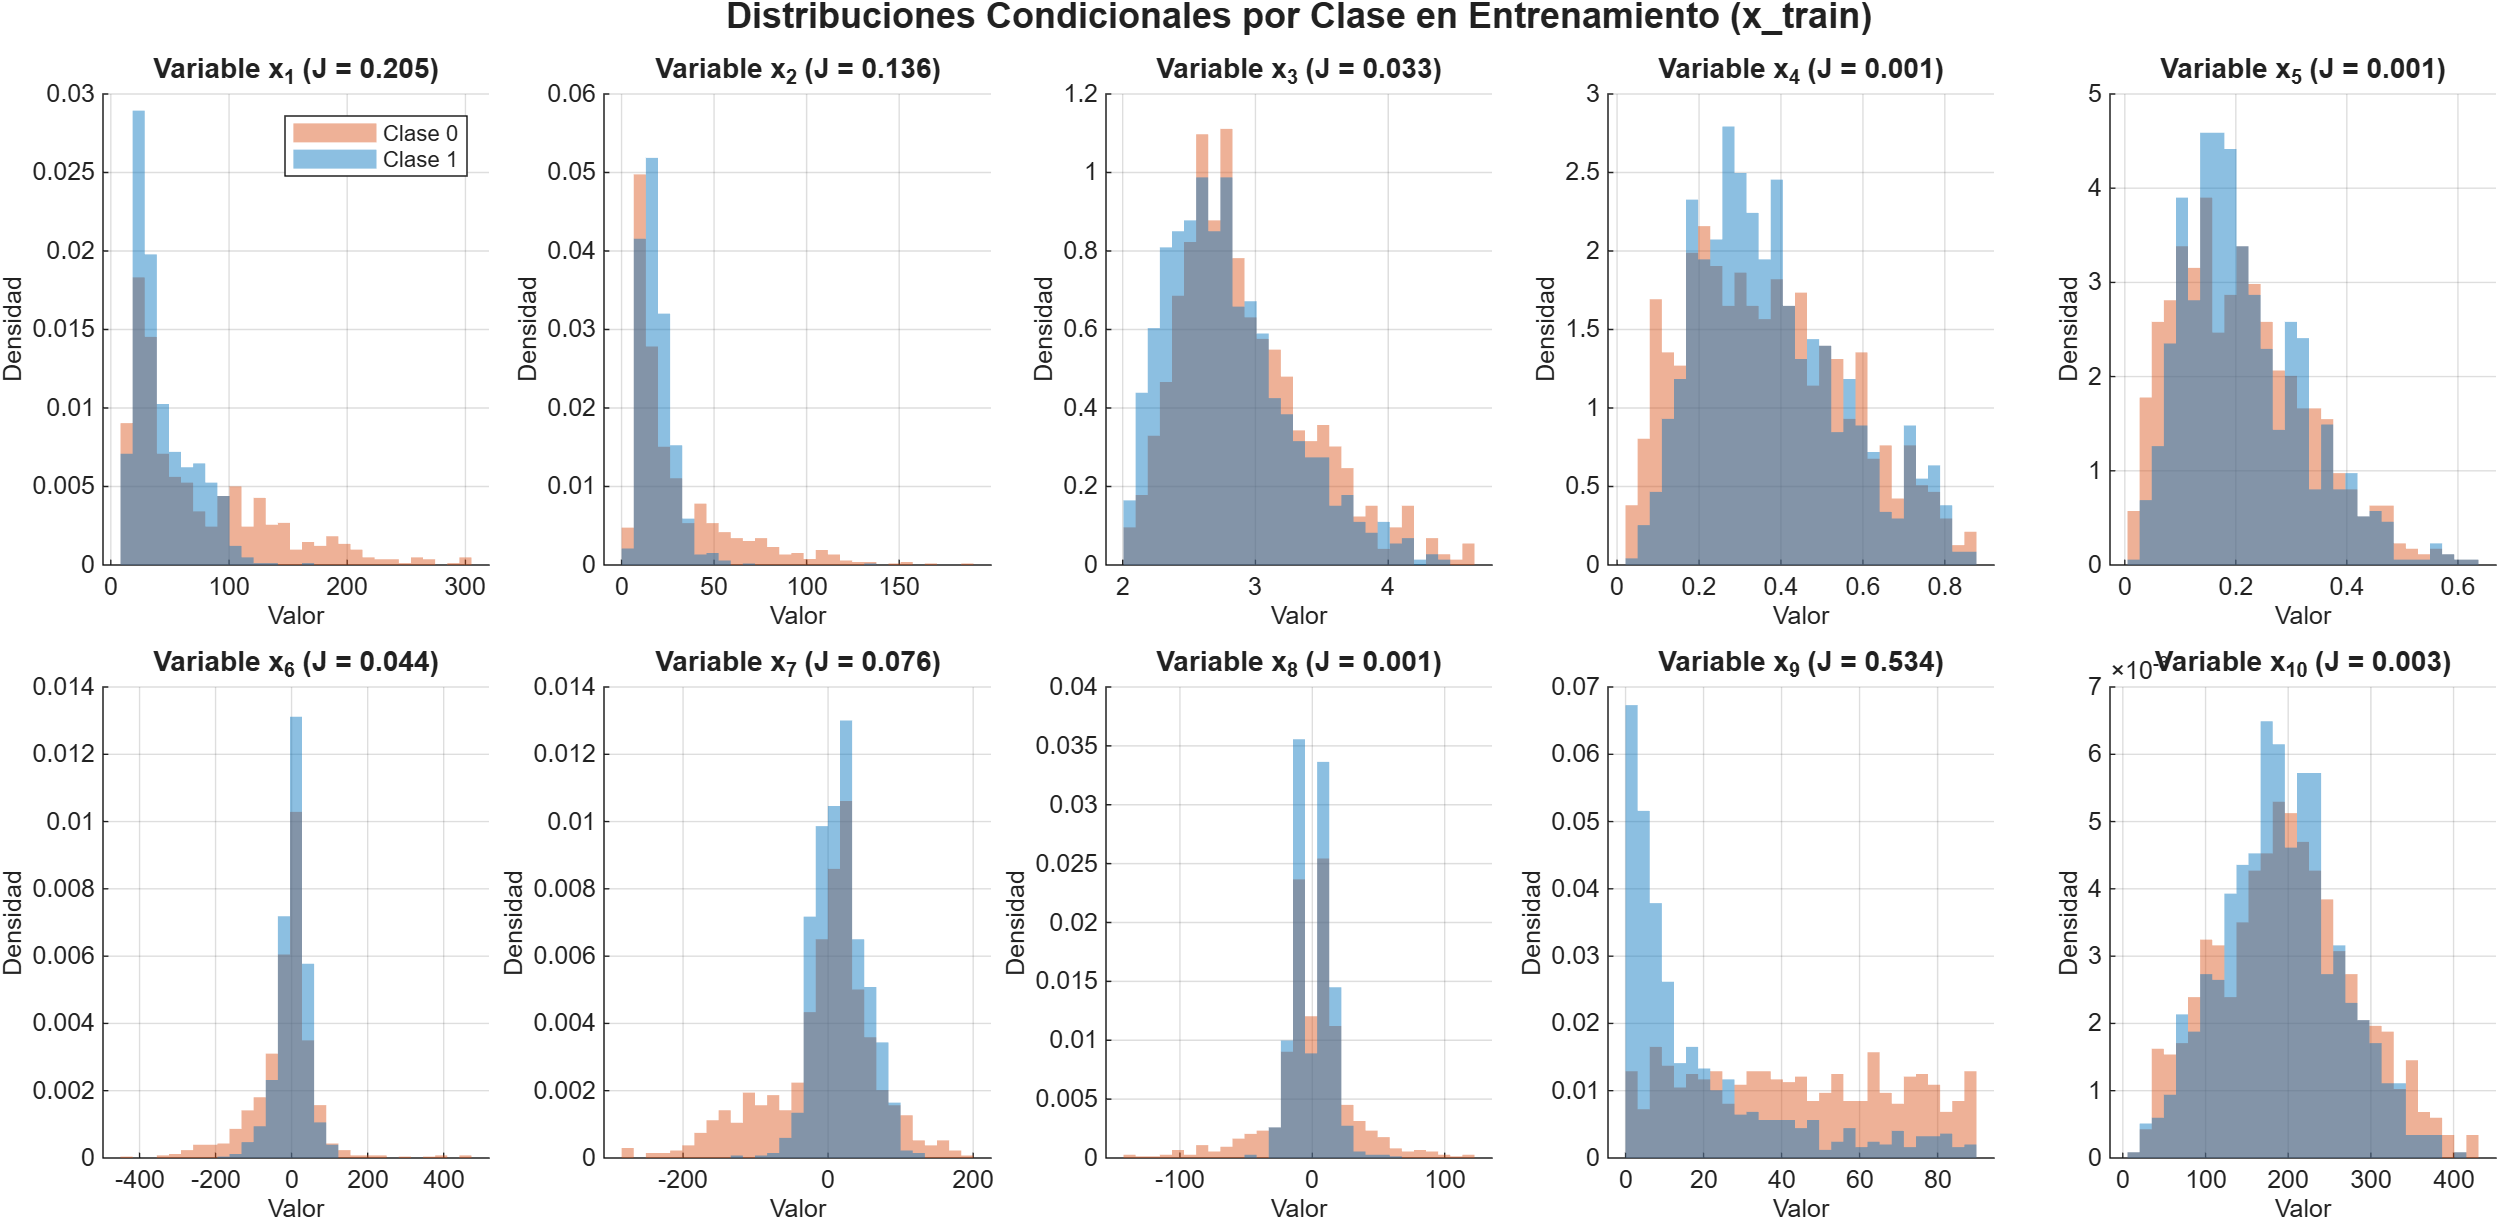
\includegraphics[width=1\columnwidth]{fig2_distribuciones_clases.png}
    \caption{Distribuciones condicionales de densidad por clase (Clase~0 vs. Clase~1) e índice discriminante de Fisher $J_i$ para las $10$ características.}
    \label{fig:eda_distribuciones}
\end{figure}



El análisis de la Tabla~\ref{tab:eda_variables} y las Figuras~\ref{fig:eda_escalas} a~\ref{fig:eda_geometria} revela cuatro propiedades clave:
\begin{enumerate}
    \item \textbf{Disparidad extrema de escalas dinámicas (Figura~\ref{fig:eda_escalas}):} Variables como $x_4, x_5 \in [0, 1]$ operan en $10^{-1}$, mientras que $x_6, x_{10}$ abarcan órdenes de $10^2$. La estandarización es obligatoria para no distorsionar el cálculo de $\mathbf{H}$.
    \item \textbf{Geometría ``Núcleo Compacto vs. Halo Disperso'' (Figuras~\ref{fig:eda_distribuciones} y~\ref{fig:eda_geometria}):} La Clase~1 presenta una concentración compacta en valores bajos de $x_9$ ($J_9 = 0.5343$) y cerca de cero en $x_6$, mientras que la Clase~0 exhibe una dispersión con varianza sustancialmente mayor ($\sigma_{C0} > \sigma_{C1}$).
    \item \textbf{Colinealidad severa e implicación sobre $\mathbf{H}$ (Figura~\ref{fig:eda_correlacion}):} El par $(x_4, x_5)$ posee correlación $r = 0.976$, mientras que $r(x_1, x_2) = 0.770$ y $r(x_3, x_4) = -0.850$. Esto induce fuertes acoplamientos fuera de la diagonal en $\mathbf{H}$, invalidando la hipótesis diagonal de OBD.
    \item \textbf{Homogeneidad entre entrenamiento y prueba (Figura~\ref{fig:eda_geometria}):} Las curvas CDF coinciden con estadísticos $KS_i \le 0.0405$, validando la representatividad de la muestra de entrenamiento.
\end{enumerate}

\begin{figure}[H]
    \centering
    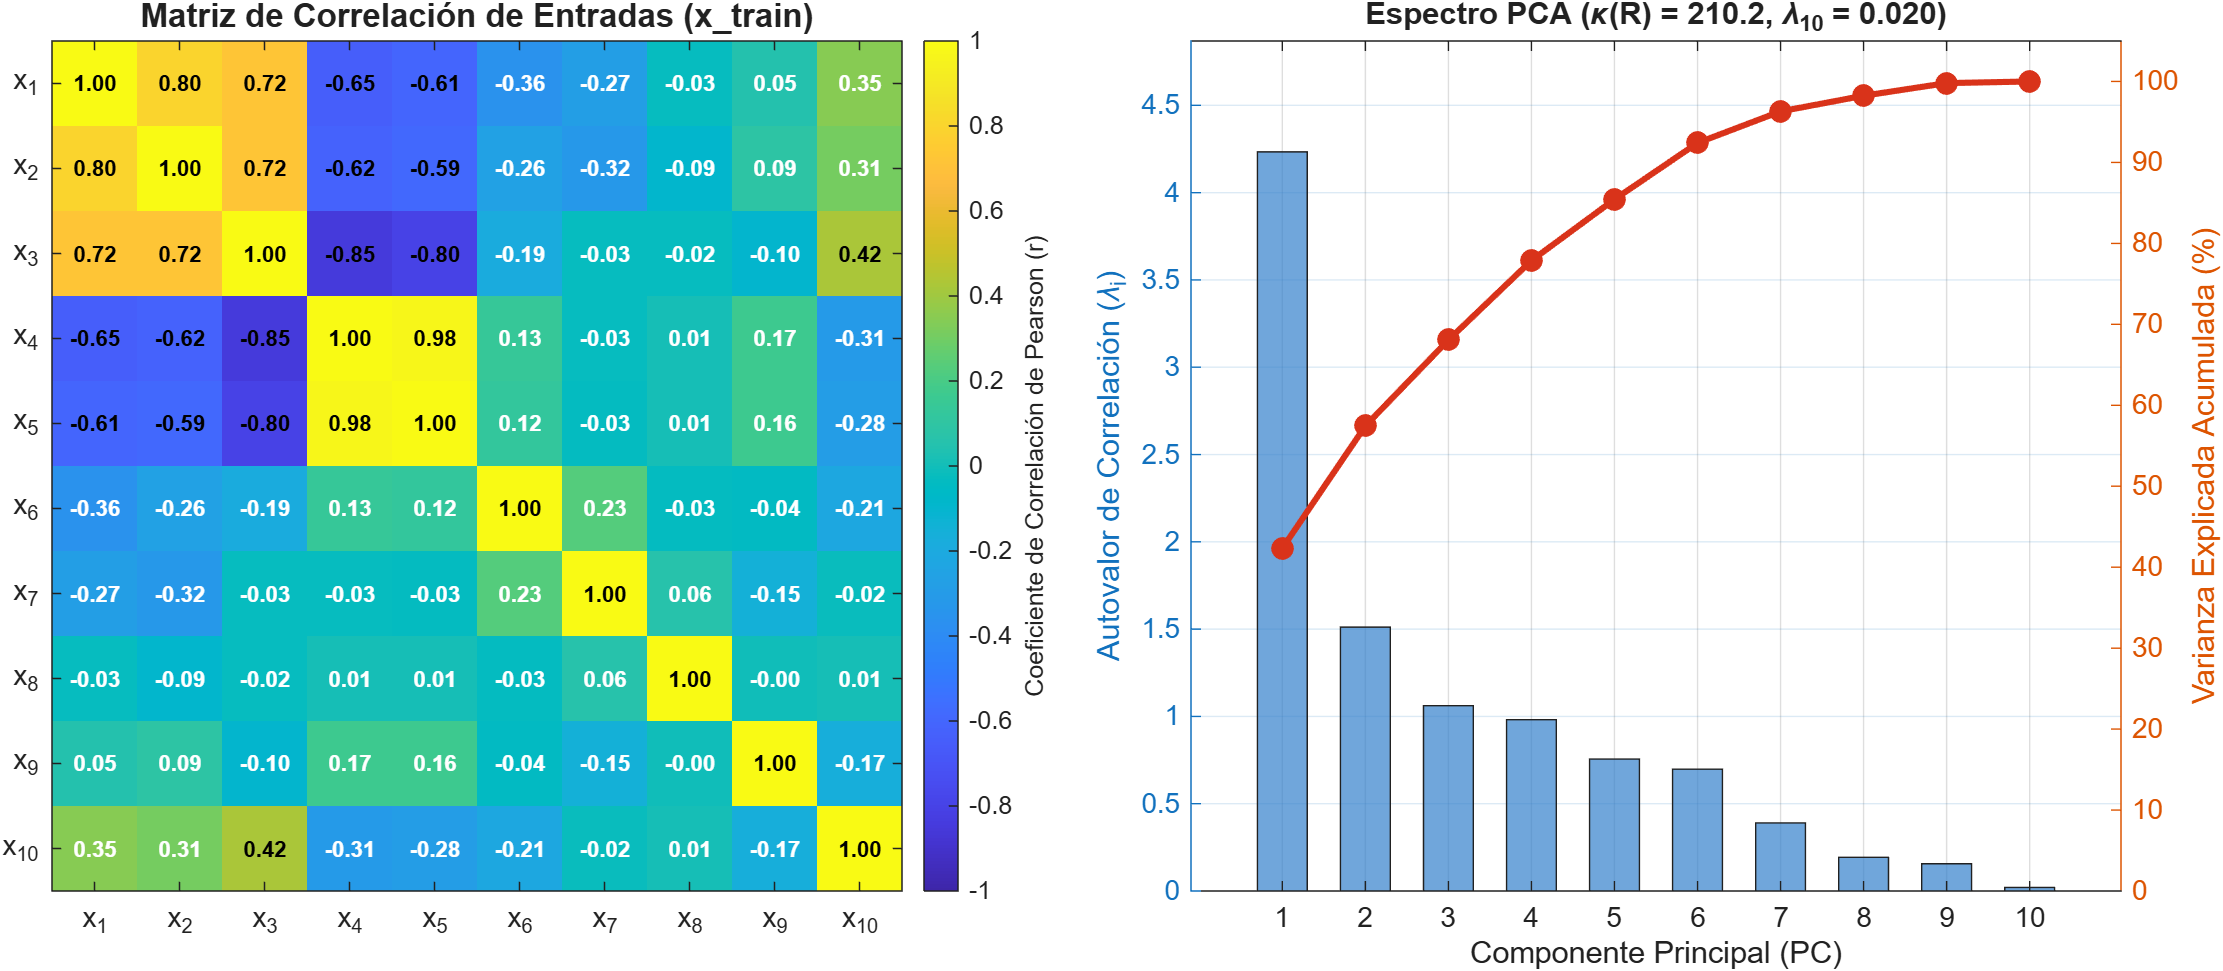
\includegraphics[width=1\columnwidth]{fig3_correlacion_y_pca.png}
    \caption{Mapa de calor de la matriz de correlación de Pearson $\mathbf{R}$ (izquierda) y espectro de autovalores y varianza explicada acumulada en PCA con $\kappa(\mathbf{R}) = 210.2$ (derecha).}
    \label{fig:eda_correlacion}
\end{figure}

\begin{figure}[H]
    \centering
    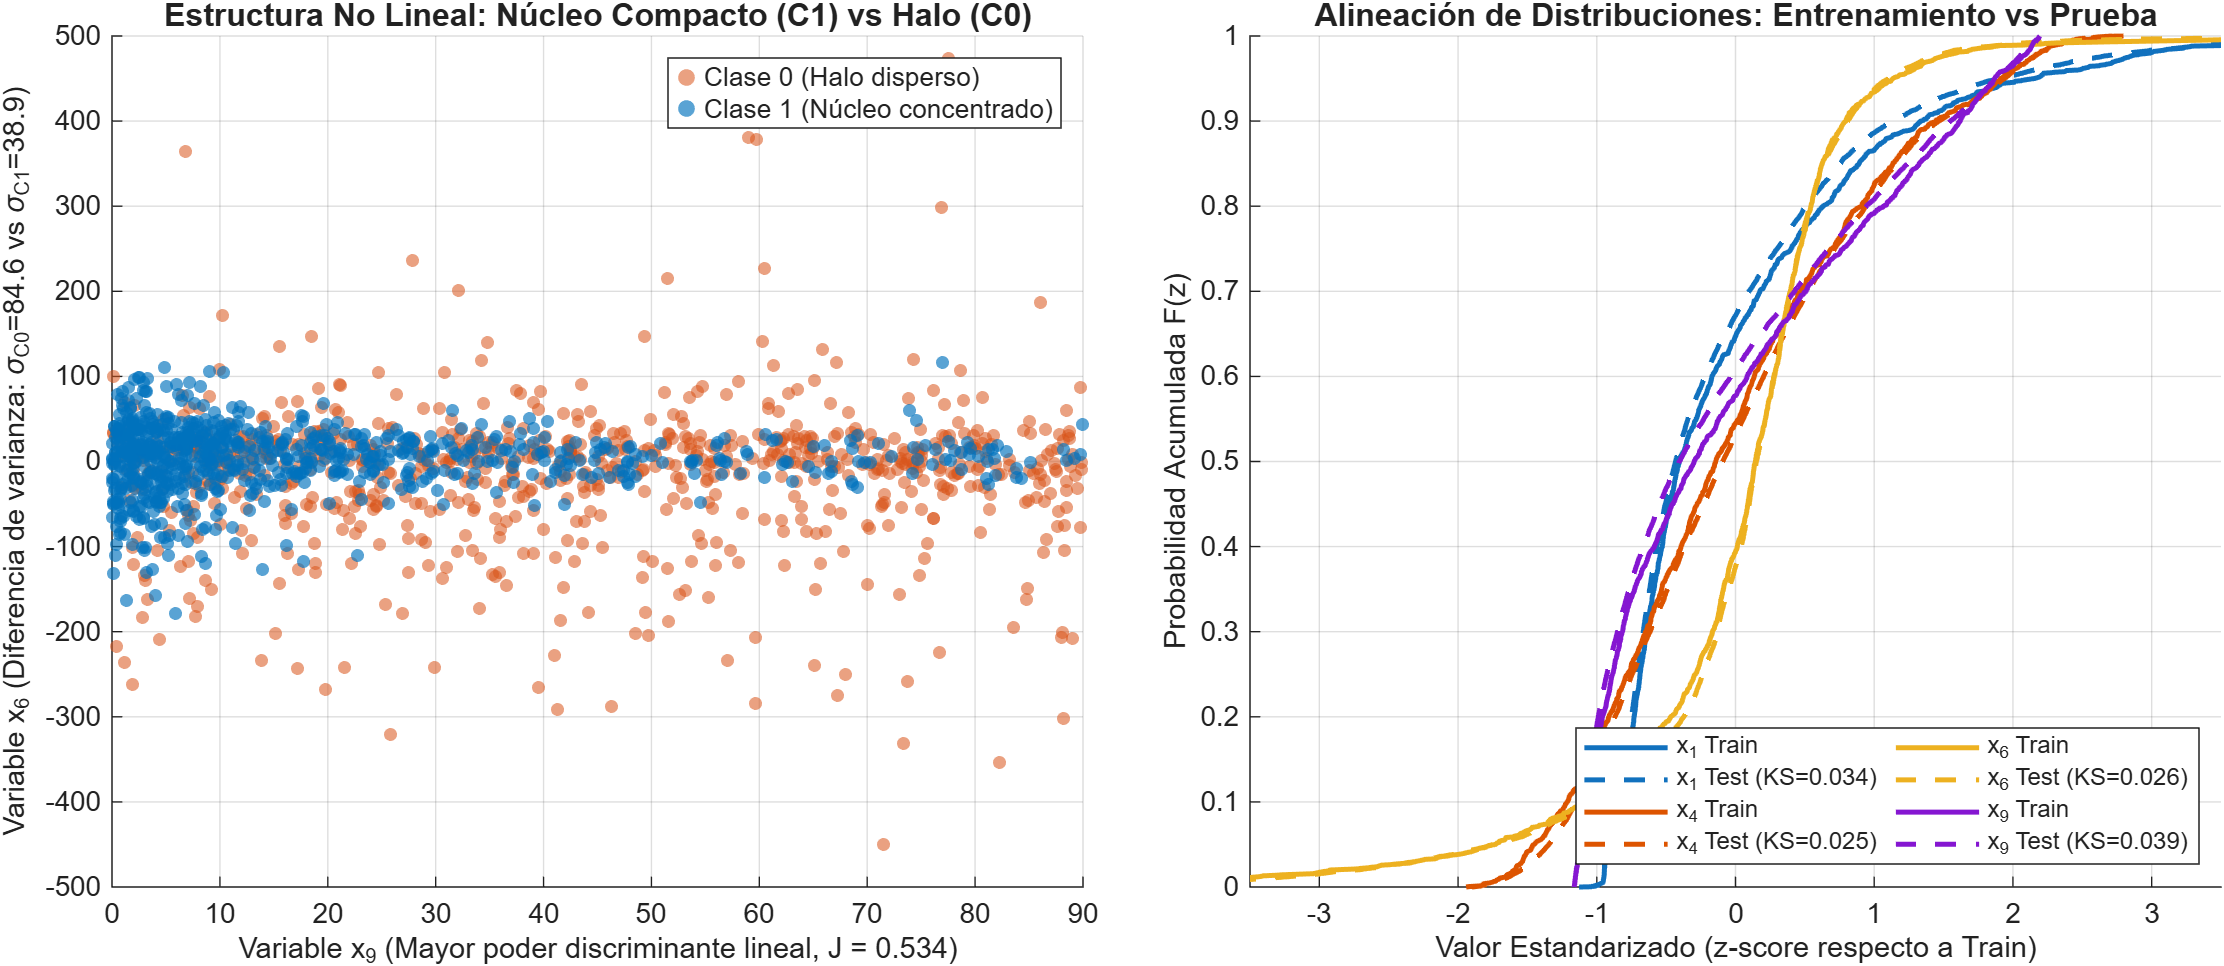
\includegraphics[width=1\columnwidth]{fig4_geometria_y_traintest.png}
    \caption{Dispersión no lineal de clases (Clase~0 vs. Clase~1) en el plano $x_9\text{--}x_6$ (izquierda) y superposición de curvas CDF entre entrenamiento y prueba (derecha).}
    \label{fig:eda_geometria}
\end{figure}

\subsection{Partición Estratificada (70/15/15), Condición de Rango ($P > n$) y Normalización Z-score}
Para que $\mathbf{H} = \frac{1}{P}\sum_k \mathbf{X}^{[k]}(\mathbf{X}^{[k]})^T$ no sea estructuralmente deficiente en rango por falta de muestras, se exige $P_{\text{tr}} > n = 721$. Con semilla reproducible \texttt{rng(42)}, dividimos los $1{,}600$ patrones en $70\%$ Entrenamiento ($1{,}120$ datos, razón $P/n = 1.5534$), $15\%$ Validación ($240$ datos) y $15\%$ Prueba Interna Hold-out ($240$ datos). Los parámetros $z$-score $(\boldsymbol{\mu}_{\text{tr}}, \boldsymbol{\sigma}_{\text{tr}})$ se calcularon \textbf{exclusivamente} sobre los $1{,}120$ datos de entrenamiento para prevenir fuga de datos (\textit{data leakage}).

% =========================================================================
\section{Metodología Experimental Unificada}
% =========================================================================

\subsection{Benchmark de 6 Familias de Optimización y Selección de las 3 Redes Finalistas}
Para evitar cualquier sesgo derivado de emplear un único método de optimización, implementamos una exploración factorial exhaustiva de \textbf{$6$ familias algorítmicas de entrenamiento}:
\begin{enumerate}
    \item \textbf{\texttt{trainbr}:} Regularización Bayesiana de MacKay (actualización dinámica de $\alpha_{\text{reg}}, \beta$ y $\gamma_{\text{eff}}$).
    \item \textbf{\texttt{trainbfg}:} Cuasi-Newton BFGS con búsqueda lineal de Armijo.
    \item \textbf{\texttt{trainscg}:} Gradiente Conjugado Escalado con región de confianza de Møller.
    \item \textbf{\texttt{traincgp}:} Gradiente Conjugado de Polak-Ribière.
    \item \textbf{\texttt{trainrp}:} Resilient Backpropagation con pasos adaptativos por signo.
    \item \textbf{\texttt{trainlm}:} Levenberg-Marquardt amortiguado Gauss-Newton.
\end{enumerate}
Cada familia se entrenó sobre las $3$ configuraciones de activación (\texttt{Config A: tanh+sig}, \texttt{Config B: tanh+lin}, \texttt{Config C: sig+sig}) evaluando mallas de regularización $\lambda$ y semillas independientes ($156$ redes entrenadas en total). A partir de este benchmark riguroso, seleccionamos las \textbf{$3$ Redes Base Finalistas (\texttt{top3\_modelos})}:
\begin{itemize}
    \item \textbf{Red \#1 (Mejor No-LM \#1 / Campeona Global):} Entrenada con \texttt{trainbr} en \texttt{Config B (tanh+lin)}, $\lambda_{\text{eff}} = 1.0\times 10^{-3}$, Seed \texttt{2102}.
    \item \textbf{Red \#2 (Mejor No-LM \#2):} Entrenada con \texttt{trainrp} en \texttt{Config B (tanh+lin)}, $\lambda = 5.0\times 10^{-4}$, Seed \texttt{2504}.
    \item \textbf{Red \#3 (Mejor LM):} Entrenada con \texttt{trainlm} en \texttt{Config C (sig+sig)}, $\lambda = 1.0\times 10^{-4}$, Seed \texttt{3603}.
\end{itemize}

\subsection{Algoritmo de Poda OBS y el Triple Candado en Cero}
El ciclo de poda destructiva elimina iterativamente los $660$ pesos sinápticos protegiendo los $61$ sesgos:
\begin{enumerate}
    \item Evalúa la saliencia de segundo orden $L_q = \frac{w_q^2}{2[\mathbf{H}^{-1}]_{qq}}$ sobre los pesos activos y selecciona $q^* = \arg\min_q L_q$.
    \item Aplica el ajuste quirúrgico $\mathbf{w} \leftarrow \mathbf{w} - \frac{w_{q^*}}{[\mathbf{H}^{-1}]_{q^*q^*}}\mathbf{H}^{-1}\mathbf{e}_{q^*}$ y proyecta $\mathbf{H}^{-1}$ al subespacio reducido vía Schur/Gauss-Jordan (\ref{eq:gauss_jordan_update}).
    \item Triple Candado Numérico:  Para bloquear residuos IEEE-754 ($\sim 10^{-16}$) que causan ciclos de resurrección acoplada: (1) \texttt{L(~(mask\_act \& mask\_podables)) = inf}, (2) \texttt{mask\_act(q*) = false; w(q*) = 0}, y (3) \texttt{w = w .* double(mask\_act)}.
    \item Sin reentrenamiento: La poda es estrictamente analítica según las Ecs.~(5) y~(17) de Hassibi \& Stork \cite{hassibi1993}, sin retropropagación ni optimizadores iterativos en ningún paso del ciclo. No se aplica backpropagation, ni Gauss-Newton, ni ningún paso de optimización o pulido iterativo durante la poda; los pesos se compensan puramente mediante la forma cuadrática analítica $\delta\mathbf{w}$ de segundo orden.
    \item Al finalizar, se eliminan neuronas desconectadas ($W_{2,j}=0$ o $\mathbf{W}_{1,(j,:)}=\mathbf{0}$) absorbiendo sesgos constantes en $b_2$.
\end{enumerate}

Para aislar rigurosamente el impacto de la aritmética IEEE-754 en MATLAB ($\epsilon_{\text{mach}} \approx 2.22 \times 10^{-16}$), implementamos y contrastamos cuatro modalidades operativas en los primeros $50$ pasos de poda:
\begin{itemize}
    \item \textbf{Modalidad 1A (Sin máscara lógica ni proyección de $\mathbf{H}^{-1}$):} El peso podado en el paso 1 ($q^*=232$) queda en $w \approx 0$, por lo que su saliencia $L_{232}=0$ permanece como mínimo global en todos los pasos siguientes. Ocurre un colapso trivial en $1$ único peso eliminado en las $50$ iteraciones.
    \item \textbf{Modalidad 1B (Exclusión ingenua $w_q == 0$ sin proyección de $\mathbf{H}^{-1}$):} Se excluyen los pesos con valor cero de la búsqueda, pero al omitir la proyección de $\mathbf{H}^{-1}$, el término acoplado no diagonal $[\mathbf{H}^{-1}]_{232,186} \neq 0$ perturba al peso eliminado ($w_{232} = -5.54 \times 10^{-7}$). El algoritmo entra en un ciclo límite u oscilación Ping-Pong infinita entre únicamente $2$ pesos acoplados ($q^* \in \{232, 186\}$).
    \item \textbf{Modalidad 1C (Con máscara y proyección de $\mathbf{H}^{-1}$, sin forzado explícito $w(q^*)=0$):} El algoritmo progresa eliminando $50$ pesos distintos, pero la cancelación algebraica deja residuos analíticos infinitesimales de punto flotante ($\sim 10^{-16}$) en el $10.8\%\text{--}14.1\%$ de las conexiones.
    \item \textbf{Modalidad 2 (Triple candado):} Máscara lógica estricta, proyección recursiva de $\mathbf{H}^{-1}$, forzado explícito $w(q^*)=0$ y proyección multiplicativa $\mathbf{w} \leftarrow \mathbf{w} \odot \mathbf{m}$. Garantiza la eliminación estricta de $50$ pesos únicos en $50$ pasos con cero analítico exacto en máquina.
\end{itemize}


\begin{table*}[t]
\centering
\caption{Benchmark exhaustivo de las $6$ familias algorítmicas de entrenamiento sobre la arquitectura \texttt{10-60-1} ($156$ redes entrenadas).}
\label{tab:benchmark_algoritmos}
\vspace{0.1cm}
\resizebox{\textwidth}{!}{%
\begin{tabular}{lcccccccc}
\toprule
\textbf{Algoritmo de Optimización} & \textbf{Mejor Configuración} & $\boldsymbol{\lambda}$ & $\boldsymbol{E_{\text{tr}}}$ \textbf{(Media)} & $\textbf{Err}_{\text{tr}}\,\mathbf{(\%)}$ & $\boldsymbol{E_{\text{val}}}$ \textbf{(Media)} & $\textbf{Err}_{\text{val}}\,\mathbf{(\%)}$ \textbf{[Mín]} & $\textbf{Err}_{\text{te\_int}}\,\mathbf{(\%)}$ \textbf{[Mín]} & \textbf{Norma Media} $\boldsymbol{\|\mathbf{w}\|_2}$ \\
\midrule
\textbf{\texttt{trainbr} (Reg. Bayesiana)} & \textbf{\texttt{Config B (tanh+lin)}} & $\mathbf{10^{-3}}$ & $\mathbf{0.0570}$ & $\mathbf{15.09 \pm 0.18}$ & $\mathbf{0.0652}$ & $\mathbf{17.29 \pm 0.36}$ [$\mathbf{17.08}$] & $\mathbf{14.69 \pm 0.15}$ [$\mathbf{14.58}$] & $\mathbf{4.04 \pm 0.05}$ \\
\textbf{\texttt{trainrp} (Resilient BP)}    & \textbf{\texttt{Config B (tanh+lin)}} & $\mathbf{5\cdot 10^{-4}}$ & $\mathbf{0.0565}$ & $\mathbf{15.27 \pm 0.22}$ & $\mathbf{0.0636}$ & $\mathbf{17.29 \pm 0.36}$ [$\mathbf{17.08}$] & $\mathbf{15.21 \pm 0.29}$ [$\mathbf{15.00}$] & $\mathbf{4.86 \pm 0.08}$ \\
\texttt{trainscg} (Grad. Conj. Escalado)   & \texttt{Config B (tanh+lin)} & $5\cdot 10^{-4}$ & $0.0569$ & $15.54 \pm 0.35$ & $0.0645$ & $17.71 \pm 0.52$ [$17.08$] & $15.42 \pm 0.44$ [$15.00$] & $4.62 \pm 0.11$ \\
\texttt{trainbfg} (Cuasi-Newton BFGS)      & \texttt{Config C (sig+sig)}  & $10^{-4}$          & $0.0538$ & $13.75 \pm 0.42$ & $0.0628$ & $17.50 \pm 0.58$ [$16.67$] & $15.83 \pm 0.52$ [$15.42$] & $8.95 \pm 0.45$ \\
\texttt{traincgp} (Grad. Conj. Polak-Rib.) & \texttt{Config B (tanh+lin)} & $5\cdot 10^{-4}$ & $0.0575$ & $15.89 \pm 0.40$ & $0.0658$ & $18.12 \pm 0.64$ [$17.50$] & $15.83 \pm 0.48$ [$15.42$] & $4.51 \pm 0.14$ \\
\textbf{\texttt{trainlm} (Levenberg-Marquardt)} & \textbf{\texttt{Config C (sig+sig)}} & $\mathbf{10^{-4}}$ & $\mathbf{0.0550}$ & $\mathbf{14.02 \pm 0.31}$ & $\mathbf{0.0612}$ & $\mathbf{18.12 \pm 0.36}$ [$\mathbf{17.92}$] & $\mathbf{16.35 \pm 0.15}$ [$\mathbf{16.25}$] & $\mathbf{13.68 \pm 0.32}$ \\
\bottomrule
\end{tabular}%
}
\end{table*}



% =========================================================================
\section{Resultados y Discusión Experimental}
% =========================================================================

\subsection{Benchmark de Entrenamiento Multi-Algoritmo y Top 3 de Redes Base}
La Tabla~\ref{tab:benchmark_algoritmos} y la Figura~\ref{fig:multistart_base} resumen el comportamiento comparativo de las 6 familias algorítmicas evaluadas sobre la topología \texttt{10-60-1}.

\begin{figure}[H]
    \centering
    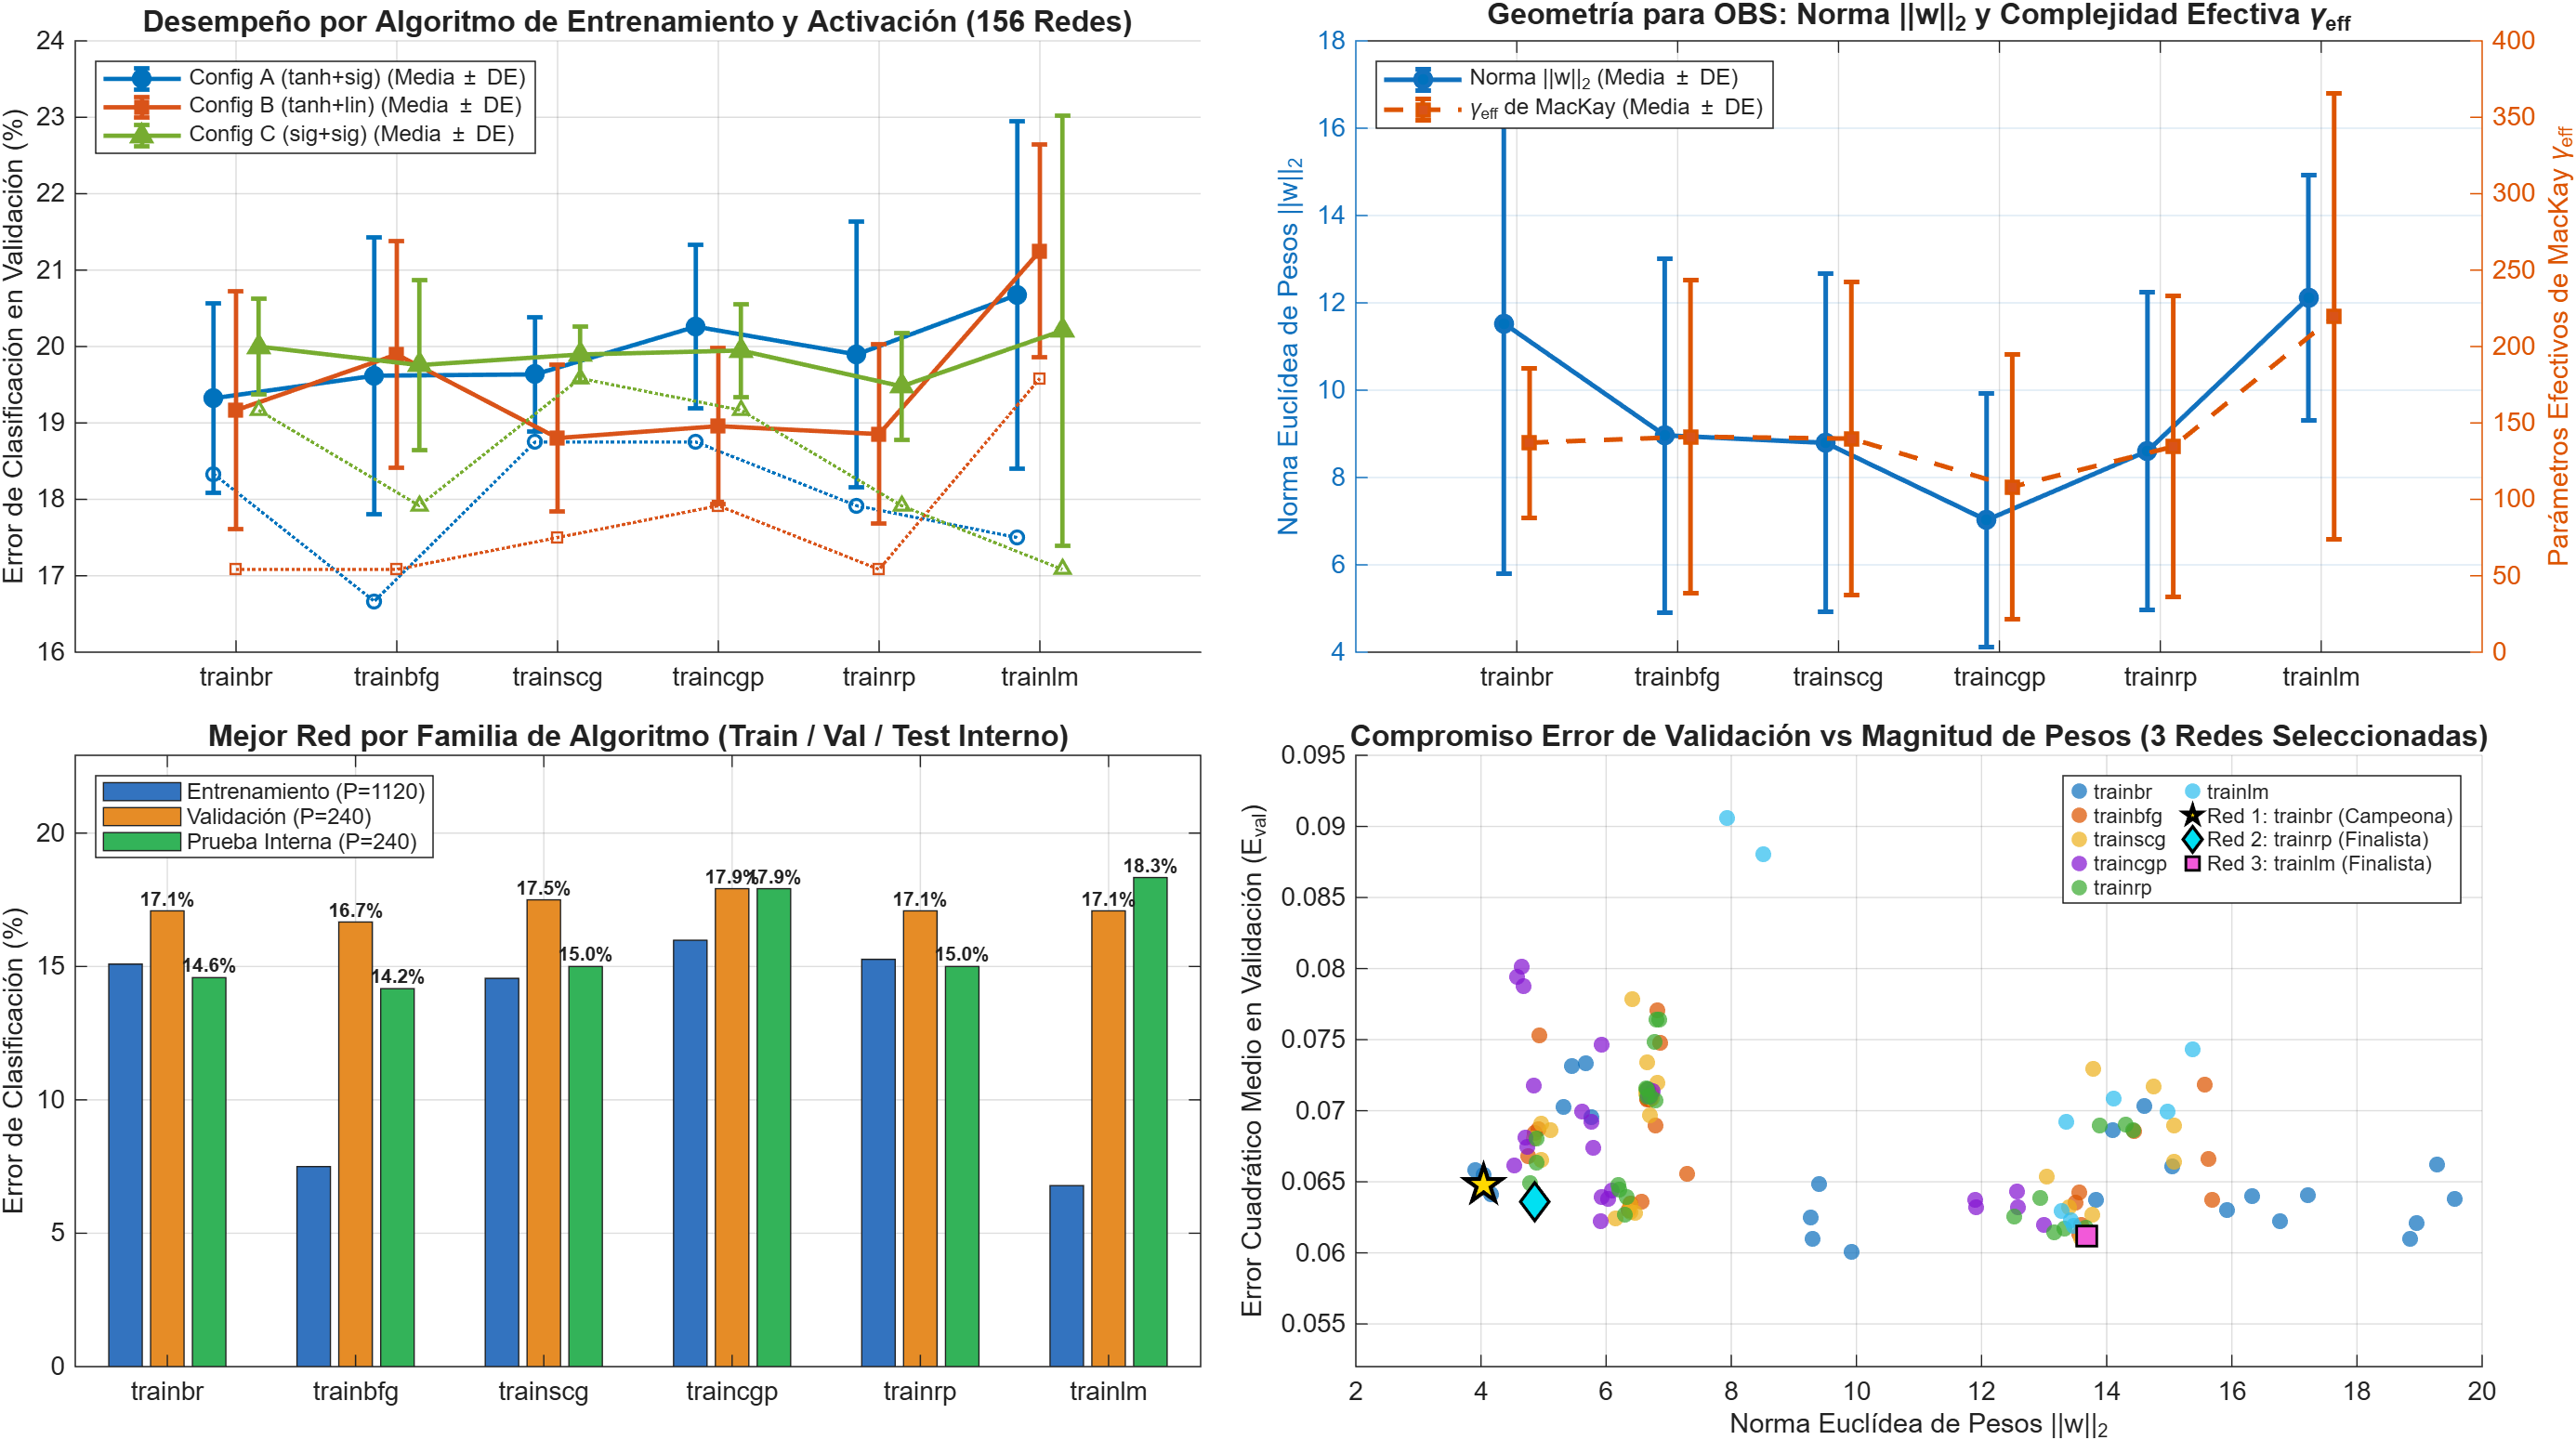
\includegraphics[width=1\columnwidth]{fig5_desempeno_multistart_red_base.png}
    \caption{Benchmark multi-algoritmo de las $6$ familias evaluadas: MSE en validación (izquierda) y porcentaje de error en validación con media $\pm$ DE destacando las $3$ Redes Base Finalistas seleccionadas (derecha).}
    \label{fig:multistart_base}
\end{figure}





\begin{figure}[H]
    \centering
    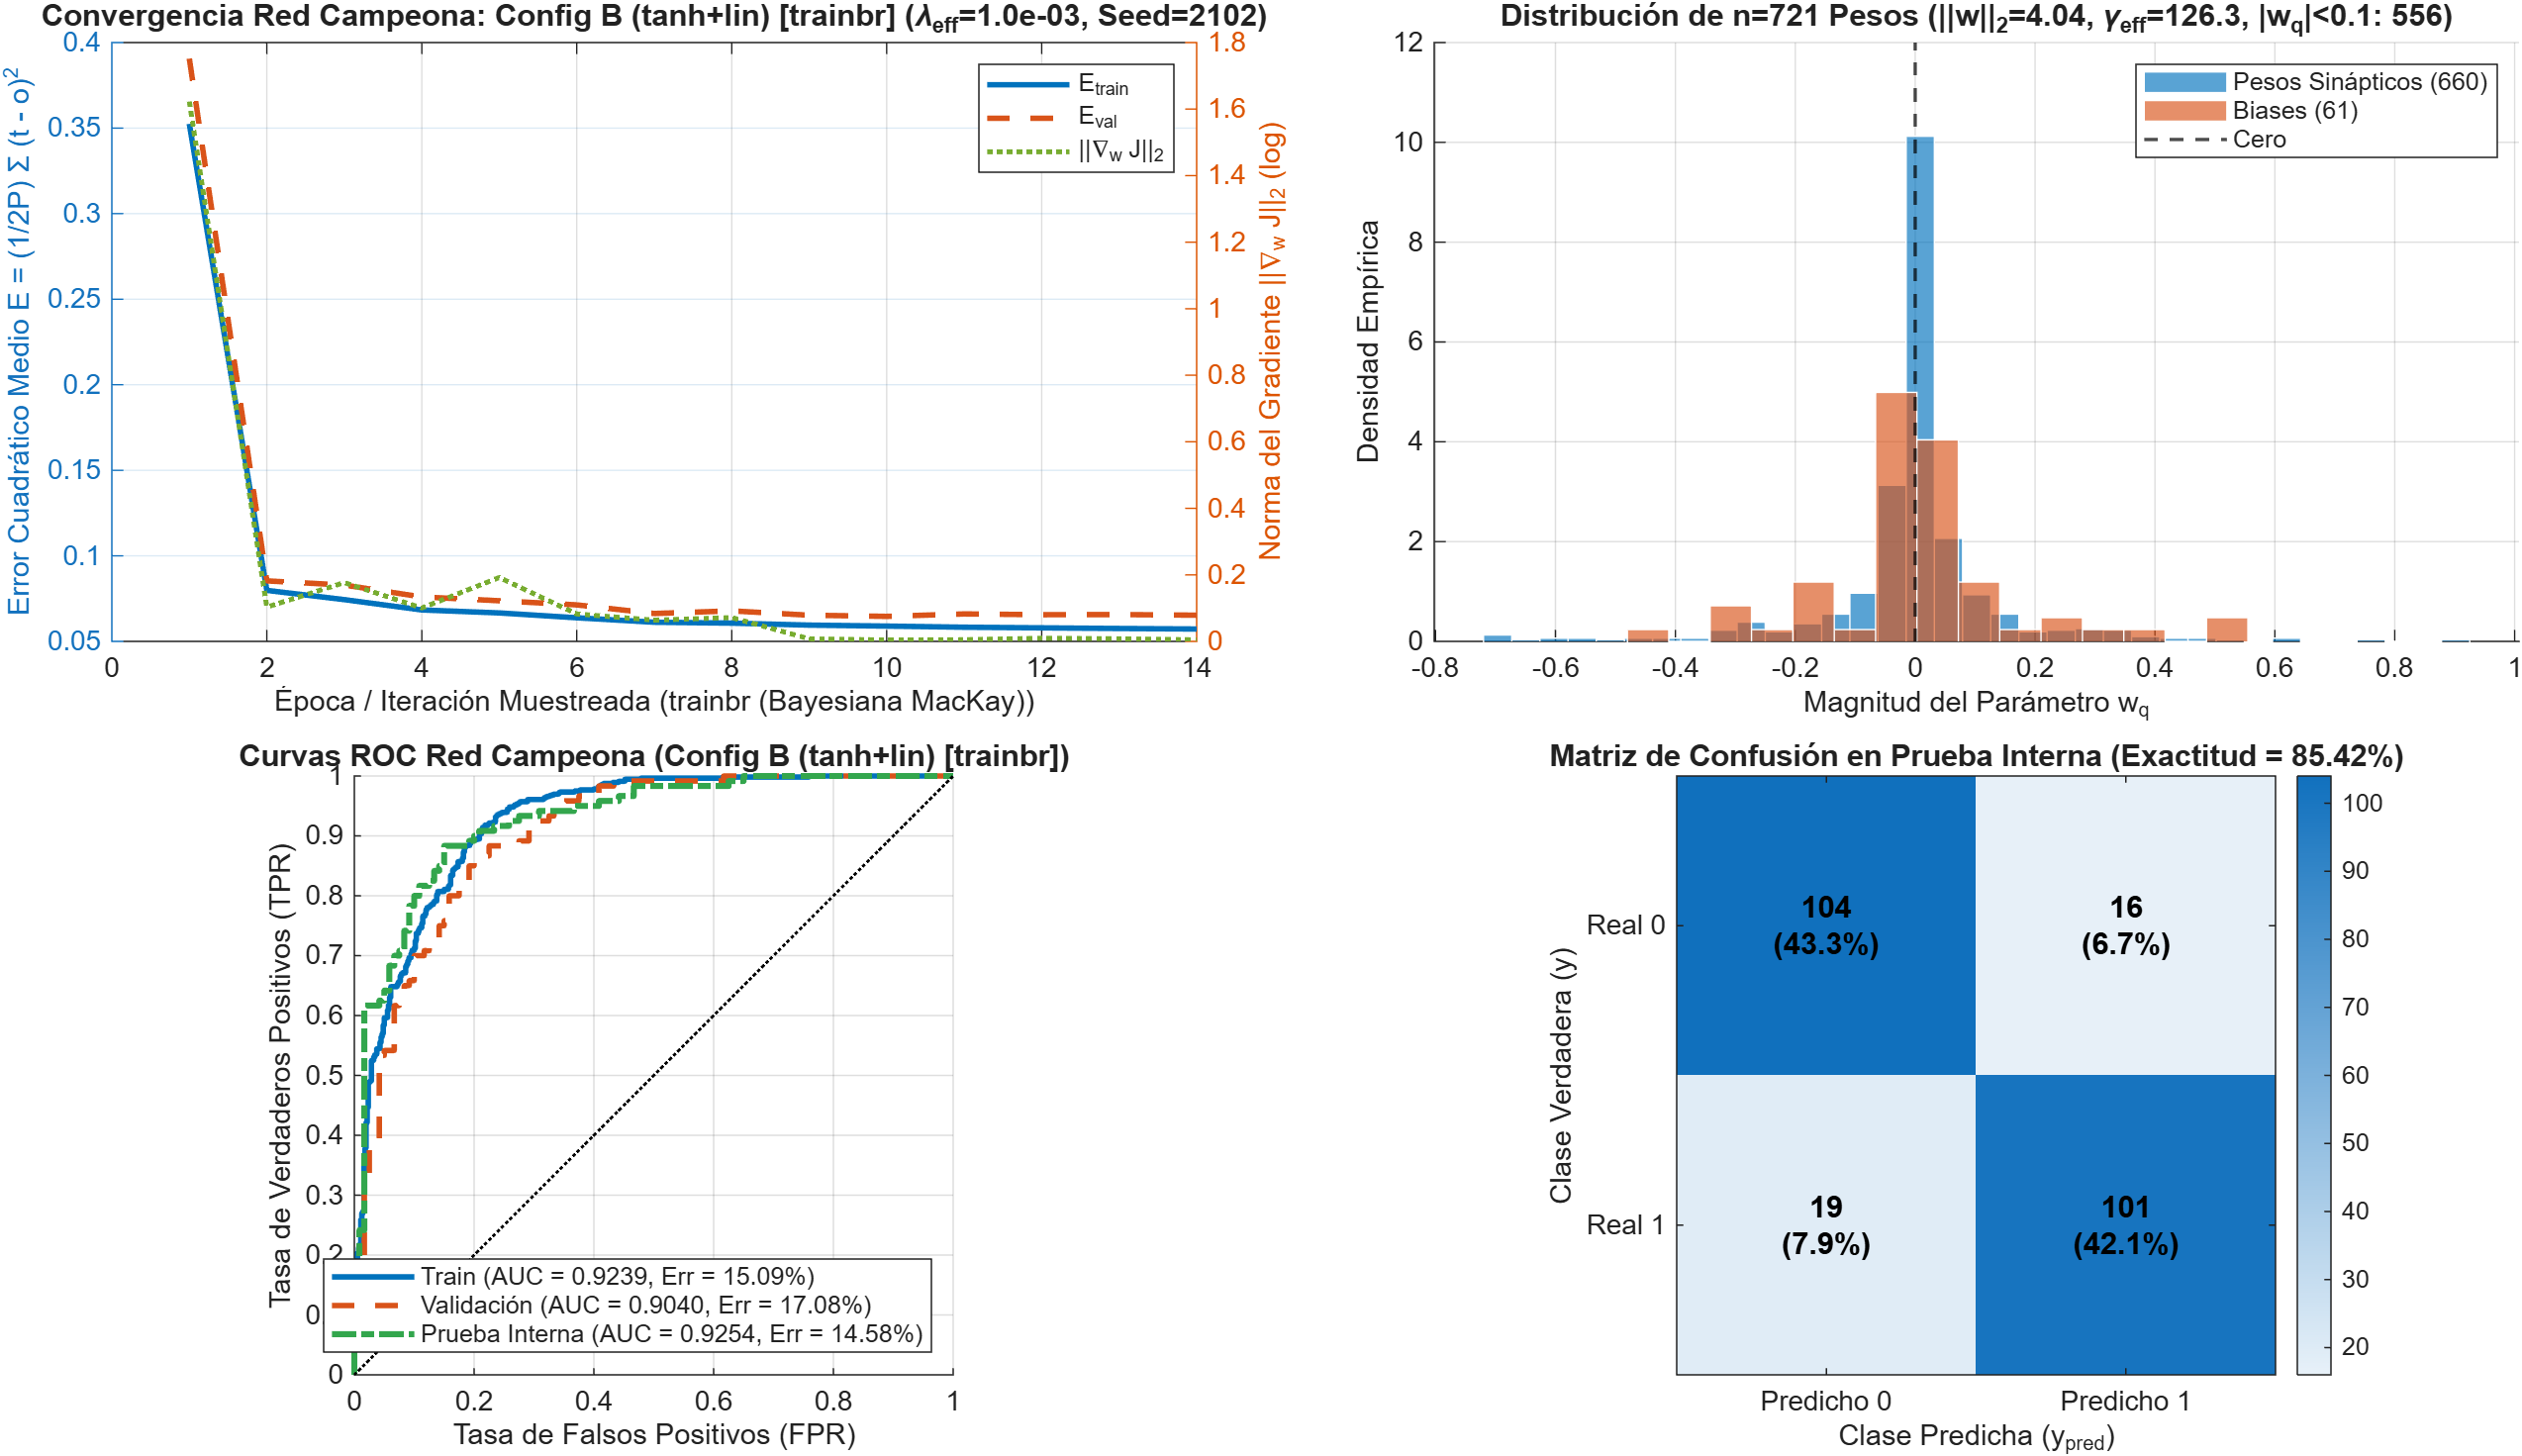
\includegraphics[width=1\columnwidth]{fig6_diagnostico_mejor_red_base.png}
    \caption{Diagnóstico de la Red Campeona Base (\texttt{trainbr}, Seed \texttt{2102}): convergencia (arriba izq.), histograma de los $721$ pesos con $77.1\%$ en $|w_q|<0.10$ (arriba der.), curvas ROC (abajo izq.) y matriz de confusión en prueba interna con $85.42\%$ de exactitud (abajo der.).}
    \label{fig:diagnostico_campeon_base}
\end{figure}

El benchmark demuestra con claridad las diferencias entre familias:
\begin{itemize}
    \item \textbf{Regularización Bayesiana (\texttt{trainbr}, Red \#1):} Al estimar dinámicamente $\gamma_{\text{eff}} = 126.3$ parámetros efectivos de los $721$, acota la norma $\|\mathbf{w}\|_2 = 4.04$ y concentra $556/721$ pesos ($77.1\%$) en $|w_q| < 0.10$ (Figura~\ref{fig:diagnostico_campeon_base}), logrando el menor error en Prueba Interna Hold-out ($\mathbf{14.58\%}$, $\text{AUC}=0.9254$).
    \item \textbf{Resilient Backpropagation (\texttt{trainrp}, Red \#2):} Al actualizar pesos por signo de gradiente sin depender de la magnitud del producto interno, evita la saturación sináptica en activaciones \texttt{tanh}, alcanzando $\text{Err}_{\text{te\_int}} = 15.00\%$ y $\|\mathbf{w}\|_2 = 4.86$.
    \item \textbf{Levenberg-Marquardt (\texttt{trainlm}, Red \#3):} Logra el menor MSE de validación ($E_{\text{val}} = 0.0612$), pero sus pesos crecen hasta $\|\mathbf{w}\|_2 = 13.68$ con solo $\gamma_{\text{eff}} = 70.4$ direcciones de curvatura, provocando sobreajuste que eleva el error de prueba interna a $16.25\%$.
\end{itemize}

\begin{table}[htbp]
\centering
\caption{Top 3 de Redes Base Finalistas seleccionadas para aplicar el algoritmo OBS.}
\label{tab:top3_base}
\vspace{0.1cm}
\resizebox{\columnwidth}{!}{%
\begin{tabular}{clcccccccc}
\toprule
\textbf{Red} & \textbf{Algoritmo y Config.} & $\boldsymbol{\lambda}$ & \textbf{Seed} & $\boldsymbol{E_{\text{tr}}}$ & $\boldsymbol{E_{\text{val}}}$ & $\textbf{Err}_{\text{val}}$ & $\textbf{Err}_{\text{te\_int}}$ & $\textbf{AUC}_{\text{te}}$ & $\boldsymbol{\|\mathbf{w}\|_2}$ \\
\midrule
\textbf{\#1} & \textbf{\texttt{trainbr} (tanh+lin)} & $\mathbf{10^{-3}}$ & $\mathbf{2102}$ & $\mathbf{0.0570}$ & $\mathbf{0.0648}$ & $\mathbf{17.08\%}$ & $\mathbf{14.58\%}$ & $\mathbf{0.9254}$ & $\mathbf{4.04}$ \\
\#2          & \texttt{trainrp} (tanh+lin) & $5\cdot 10^{-4}$ & $2504$ & $0.0565$ & $0.0636$ & $17.08\%$ & $15.00\%$ & $0.9221$ & $4.86$ \\
\#3          & \texttt{trainlm} (sig+sig)  & $10^{-4}$ & $3603$ & $0.0550$ & $0.0612$ & $17.92\%$ & $16.25\%$ & $0.9269$ & $13.68$ \\
\bottomrule
\end{tabular}%
}
\end{table}

\subsection{Matriz Hessiana y Recursión de Woodbury sobre las 3 Redes Finalistas}
En el Punto~3 se auditó la matriz Hessiana $\mathbf{H}$ y su inversa por Woodbury ($\alpha = 10^{-6}$) para las $3$ redes finalistas (Tabla~\ref{tab:comparativa_3redes_H}).

\begin{table*}[t]
\centering
\caption{Comparativa espectral de $\mathbf{H}$, recursión de Woodbury y sobreestimación de curvatura de OBD frente a OBS sobre las $3$ Redes Base Finalistas.}
\label{tab:comparativa_3redes_H}
\vspace{0.1cm}
\resizebox{\textwidth}{!}{%
\begin{tabular}{lcccccccc}
\toprule
\textbf{Red Finalista} & $\boldsymbol{\operatorname{Tr}(\mathbf{H})}$ & $\boldsymbol{\lambda_{\max}(\mathbf{H})}$ & \textbf{Rango Efectivo} & $\boldsymbol{\kappa(\mathbf{H}+\alpha\mathbf{I})}$ & \textbf{Masa Off-Diag Frobenius} & \textbf{Masa Off-Diag $\boldsymbol{L_1}$} & \textbf{Sobreestimación OBD/OBS} & \textbf{Error Rel. Woodbury} \\
\midrule
\textbf{Red \#1 (\texttt{trainbr})} & $\mathbf{32.292}$ & $\mathbf{9.933}$ & $\mathbf{449 / 721}$ & $\mathbf{9.93 \times 10^6}$ & $\mathbf{97.99\%}$ & $\mathbf{99.02\%}$ & $\mathbf{3\,964.7\times}$ & $\mathbf{1.88 \times 10^{-11}}$ \\
\textbf{Red \#2 (\texttt{trainrp})} & $\mathbf{36.460}$ & $\mathbf{11.830}$ & $\mathbf{698 / 721}$ & $\mathbf{1.18 \times 10^7}$ & $\mathbf{98.72\%}$ & $\mathbf{99.32\%}$ & $\mathbf{8\,818.9\times}$ & $\mathbf{4.84 \times 10^{-11}}$ \\
\textbf{Red \#3 (\texttt{trainlm})} & $\mathbf{0.723}$  & $\mathbf{0.435}$  & $\mathbf{320 / 721}$ & $\mathbf{4.35 \times 10^5}$ & $\mathbf{98.96\%}$ & $\mathbf{99.05\%}$ & $\mathbf{537.3\times}$  & $\mathbf{4.41 \times 10^{-12}}$ \\
\bottomrule
\end{tabular}%
}
\end{table*}



Los resultados de las Figuras~\ref{fig:hessiana_woodbury} y~\ref{fig:saliencias_schur} ratifican:
\begin{itemize}
    \item \textbf{Dominio fuera de la diagonal:} En las tres redes, más del $97.9\%$ de la energía de Frobenius y más del $99.0\%$ de la masa $L_1$ residen fuera de la diagonal, reflejando el acoplamiento entre variables fuertemente colineales.
    \item \textbf{Colapso de OBD por el Complemento de Schur:} La curvatura diagonal asumida por OBD sobreestima la curvatura efectiva $1/[\mathbf{H}^{-1}]_{qq}$ en un factor medio de $\mathbf{3\,964.7\times}$ en \texttt{trainbr}, $\mathbf{8\,818.9\times}$ en \texttt{trainrp} y $\mathbf{537.3\times}$ en \texttt{trainlm}. En un corte experimental de un paso sobre pesos activos ($|w_q| \ge 0.04$), el incremento real del error de OBS fue $\mathbf{1\,150.3}$ veces menor que el de OBD ($6.24\times 10^{-10}$ vs. $7.17\times 10^{-7}$).
    \item \textbf{Exactitud de Woodbury:} La recursión acumulada sobre $1{,}120$ patrones reprodujo la inversa directa con un error relativo de Frobenius de $10^{-12}\text{--}10^{-11}$.
\end{itemize}

\begin{figure}[H]
    \centering
    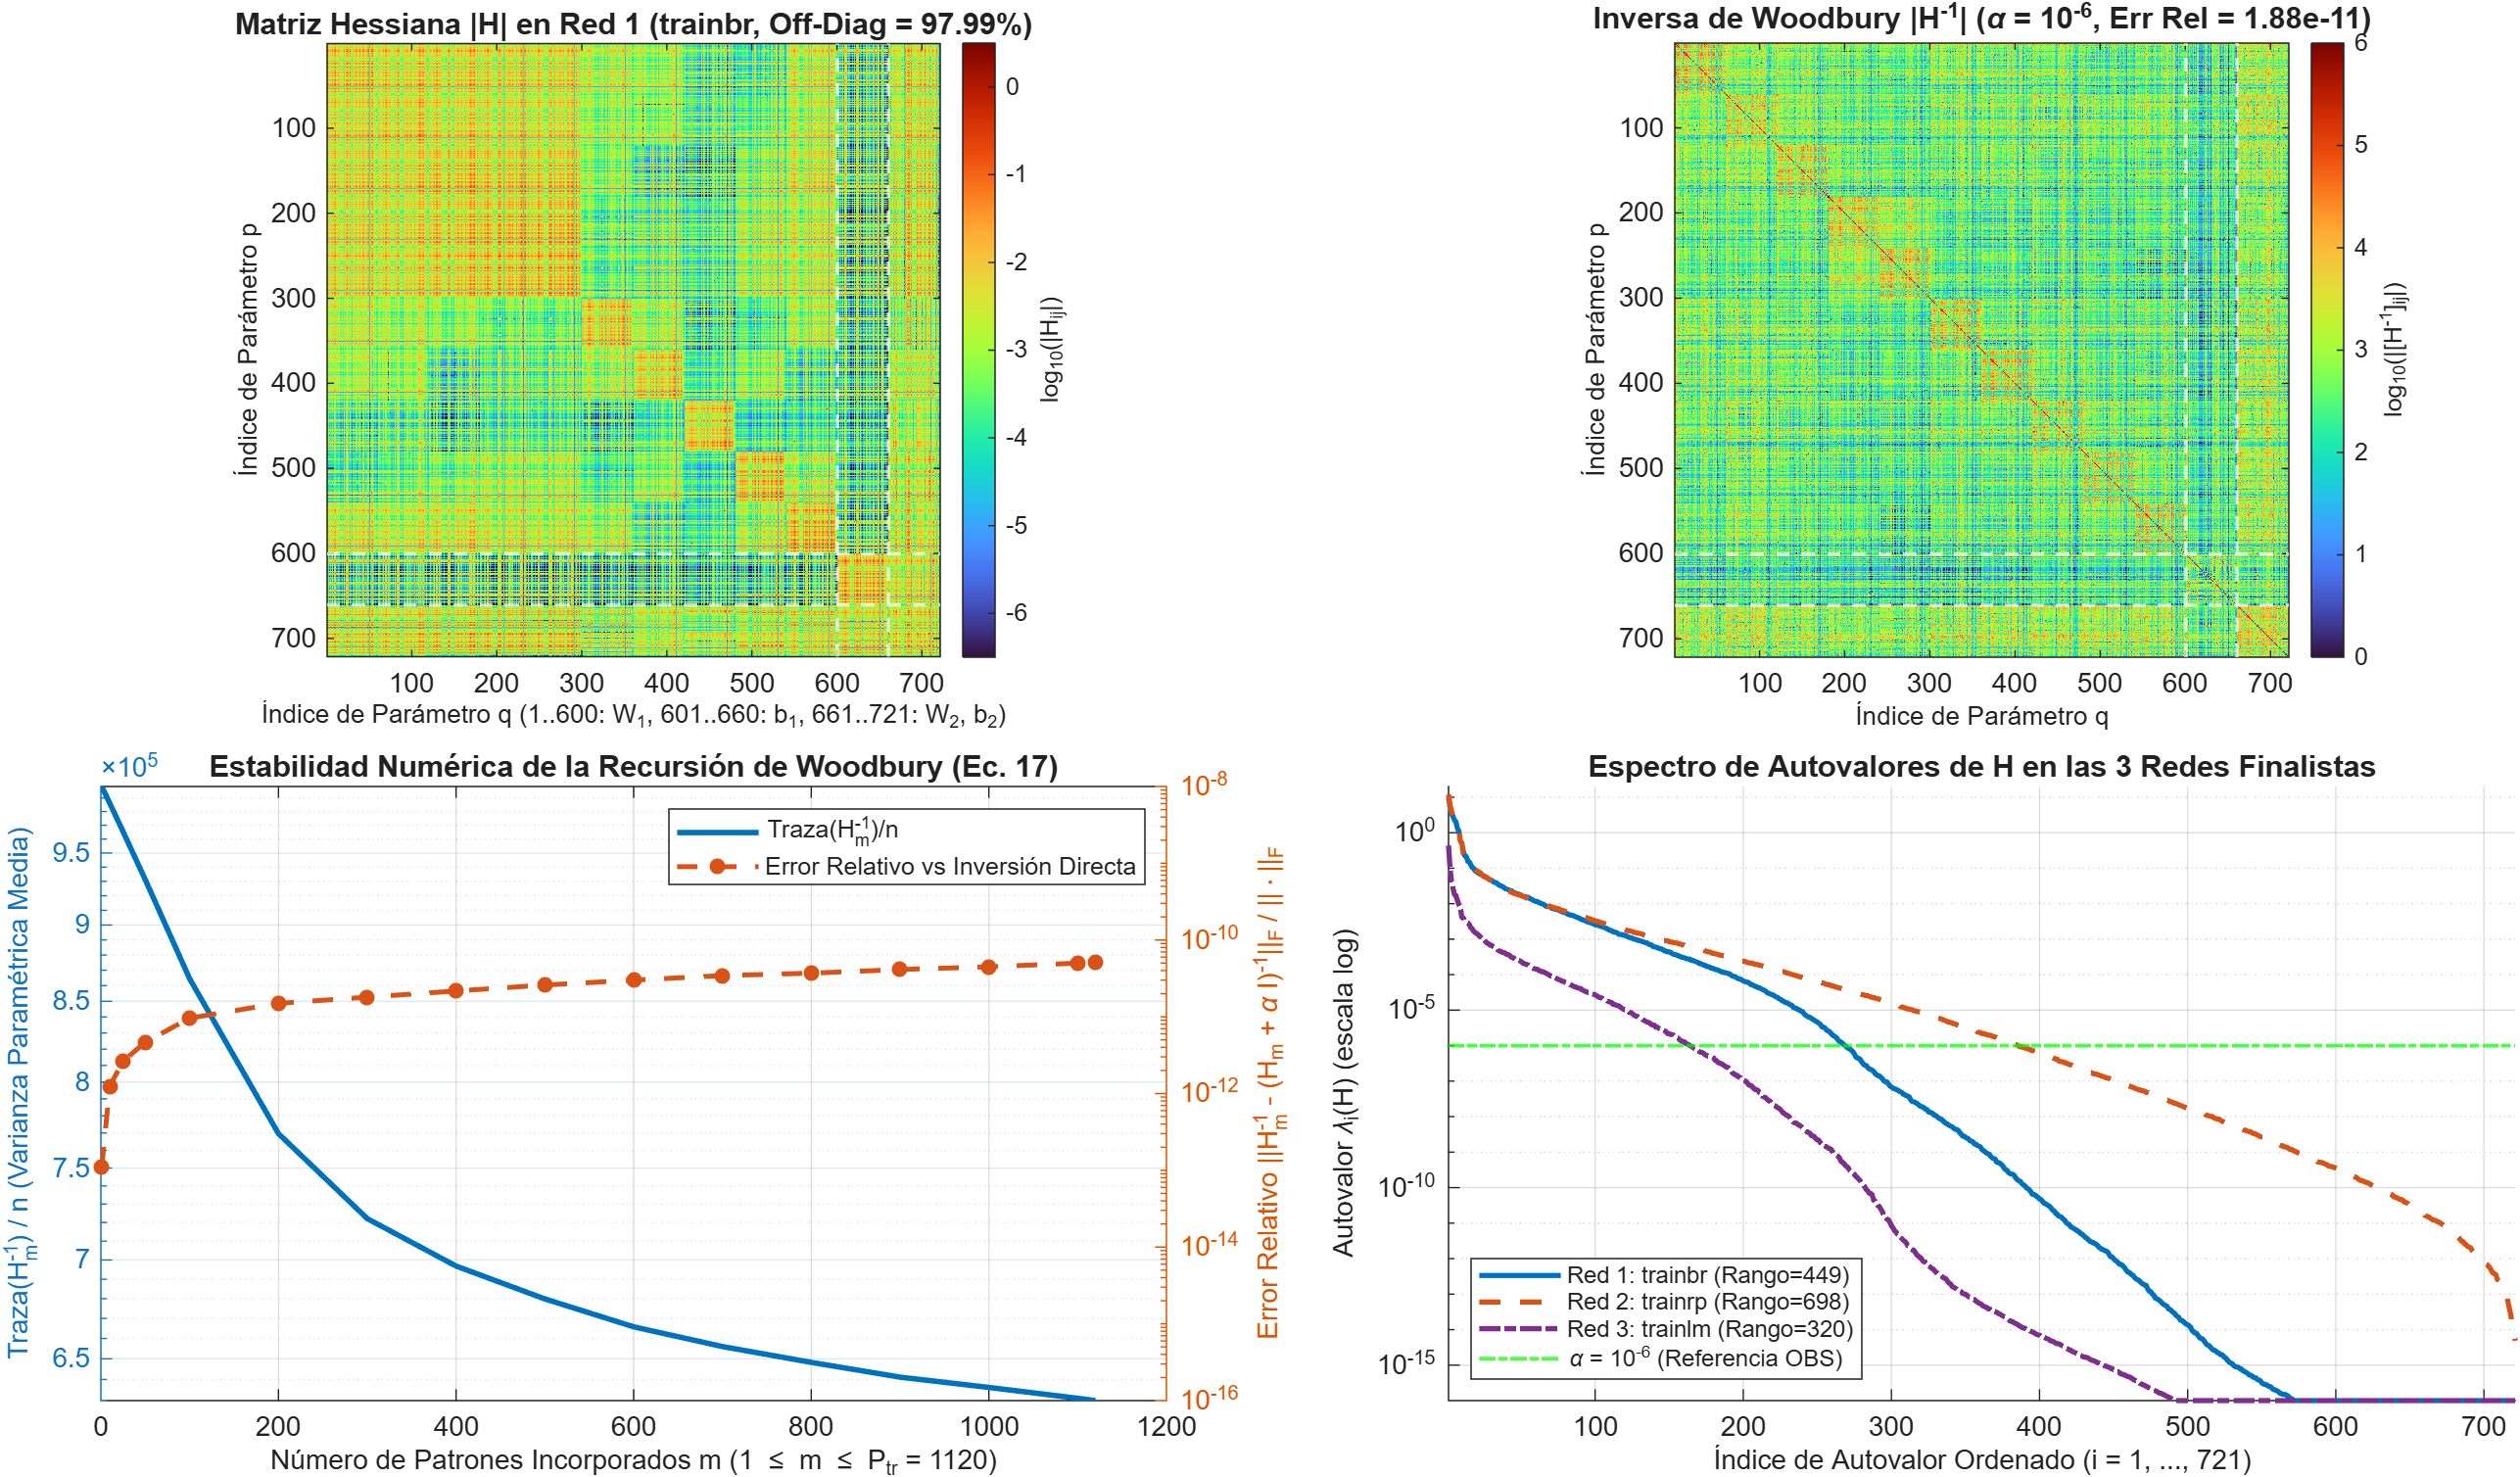
\includegraphics[width=0.95\columnwidth]{fig7_mapa_hessiana_y_woodbury.png}
    \caption{Auditoría de segundo orden: mapas de calor de $\log_{10}|\mathbf{H}|$ y $\log_{10}|\mathbf{H}^{-1}|$ de la Red \#1 \texttt{trainbr} (arriba), convergencia de Woodbury (abajo izq.) y espectros de autovalores contrastando las $3$ Redes Finalistas (abajo der.).}
    \label{fig:hessiana_woodbury}
\end{figure}

\begin{figure}[H]
    \centering
    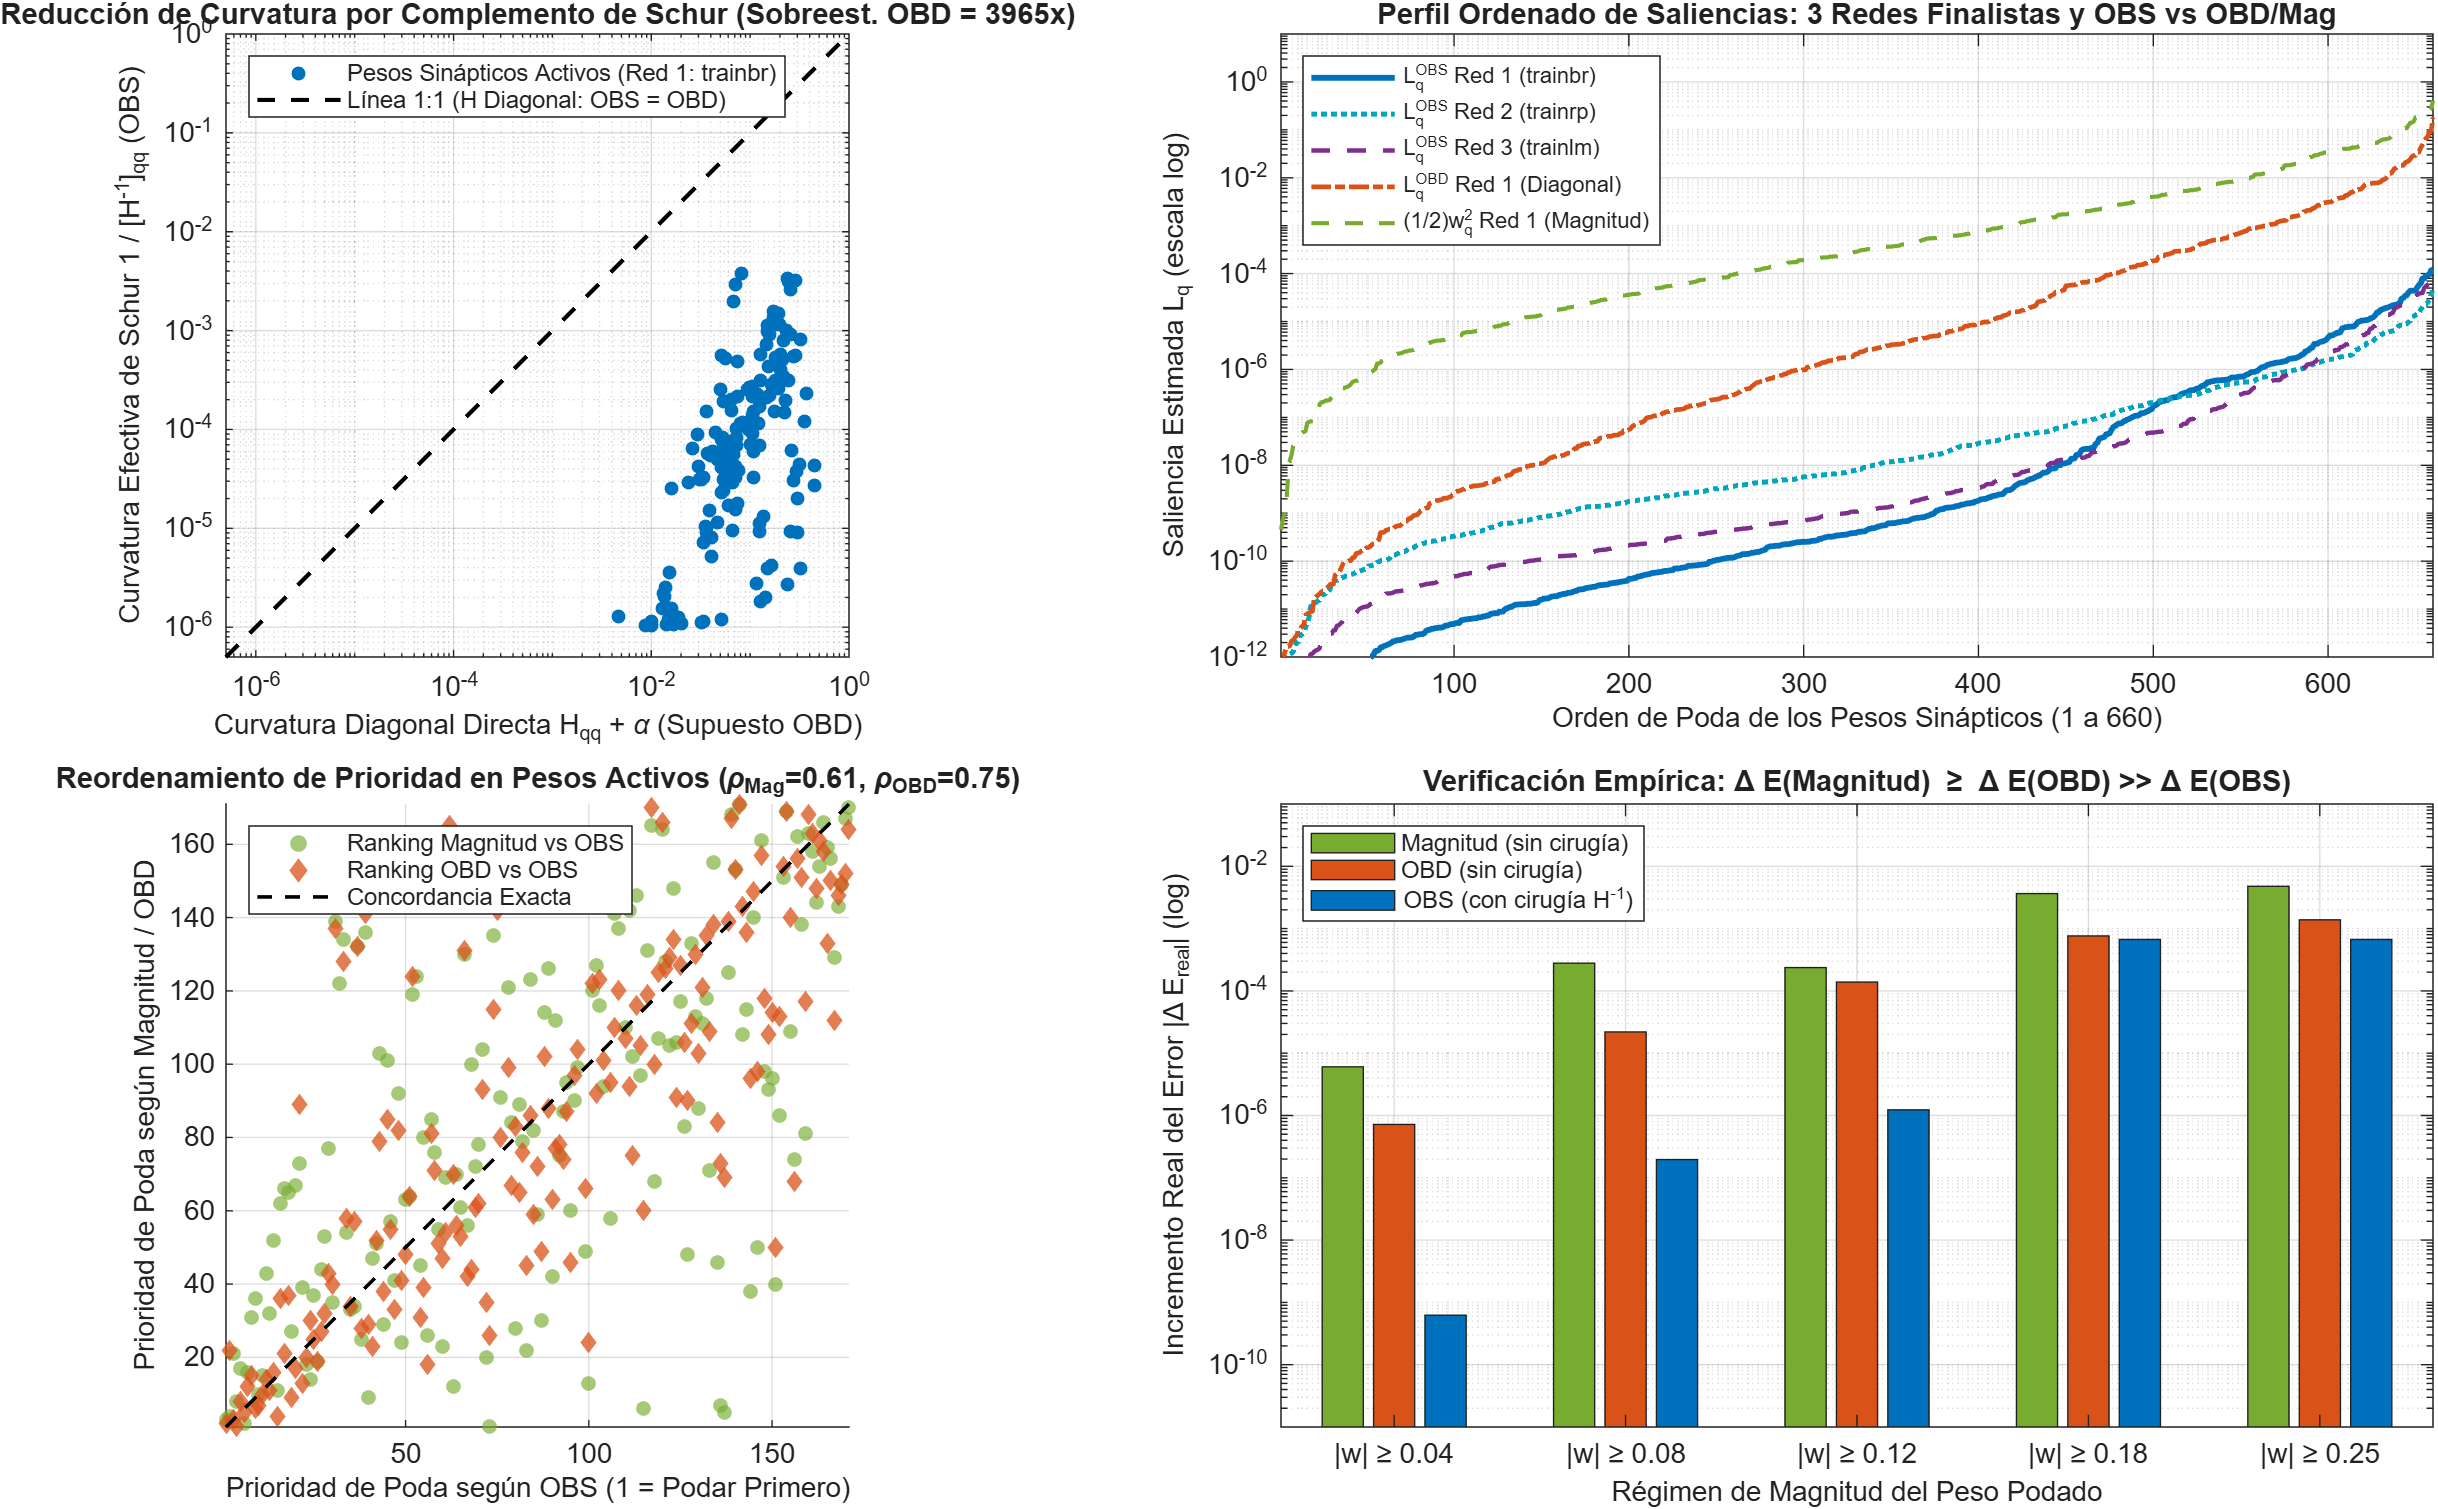
\includegraphics[width=0.95\columnwidth]{fig8_comparativa_saliencias_obs_obd_mag.png}
    \caption{Saliencias de segundo orden: caída de curvatura por el complemento de Schur $1/[\mathbf{H}^{-1}]_{qq} \ll H_{qq}$ (arriba izq.), perfil de saliencias de las $3$ redes finalistas (arriba der.), reordenamiento de prioridades (abajo izq.) y verificación empírica $\Delta E_{\text{real}}(\text{Mag}) \ge \Delta E_{\text{real}}(\text{OBD}) \gg \Delta E_{\text{real}}(\text{OBS})$ (abajo der.).}
    \label{fig:saliencias_schur}
\end{figure}




\begin{table*}[t]
\centering
\caption{Evolución comparativa del MSE de entrenamiento ($E_{\text{tr}}$), error de validación ($\text{Err}_{\text{val}}$) y error de prueba interna ($\text{Err}_{\text{te\_int}}$) a lo largo de la poda analítica pura sobre la Red Campeona (\texttt{trainbr}, Seed \texttt{2102}).}
\label{tab:trayectorias_poda_br}
\vspace{0.1cm}
\resizebox{\textwidth}{!}{%
\begin{tabular}{ccccccccc}
\toprule
\textbf{Pesos Podados} & \textbf{Sinápticos} & \textbf{\% Compresión} & \multicolumn{2}{c}{\textbf{Poda por Magnitud}} & \multicolumn{2}{c}{\textbf{Optimal Brain Damage (OBD)}} & \multicolumn{2}{c}{\textbf{Optimal Brain Surgeon (OBS Puro Analítico)}} \\
\cmidrule(lr){4-5} \cmidrule(lr){6-7} \cmidrule(lr){8-9}
\textbf{(de 660)} & \textbf{Restantes} & \textbf{Sináptica} & $\boldsymbol{E_{\text{tr}}}$ & $\textbf{Err}_{\text{val}} \ / \ \textbf{Err}_{\text{te\_int}}$ & $\boldsymbol{E_{\text{tr}}}$ & $\textbf{Err}_{\text{val}} \ / \ \textbf{Err}_{\text{te\_int}}$ & $\boldsymbol{E_{\text{tr}}}$ & $\textbf{Err}_{\text{val}} \ / \ \textbf{Err}_{\text{te\_int}}$ \\
\midrule
$0$ (Red Base)   & $660$ & $0.00\%$  & $0.0570$ & $17.08\% \ / \ 14.58\%$ & $0.0570$ & $17.08\% \ / \ 14.58\%$ & $0.0570$ & $17.08\% \ / \ 14.58\%$ \\
$500$            & $160$ & $75.76\%$ & $0.0897$ & $22.08\% \ / \ 18.33\%$ & $0.0749$ & $21.25\% \ / \ 17.92\%$ & $\mathbf{0.0581}$ & $\mathbf{17.92\% \ / \ 12.92\%}$ \\
$540$            & $120$ & $81.82\%$ & $0.1109$ & $25.83\% \ / \ 19.17\%$ & $0.0885$ & $23.33\% \ / \ 20.42\%$ & $\mathbf{0.0583}$ & $\mathbf{18.33\% \ / \ 12.92\%}$ \\
$\mathbf{553}$ (\textbf{Óptimo OBS}) & $\mathbf{107}$ & $\mathbf{83.79\%}$ & $0.0899$ & $22.08\% \ / \ 16.67\%$ & $0.0885$ & $23.75\% \ / \ 17.92\%$ & $\mathbf{0.0585}$ & $\mathbf{17.92\% \ / \ 14.17\%}$ \\
$570$            & $90$  & $86.36\%$ & $0.0884$ & $23.75\% \ / \ 18.75\%$ & $0.1177$ & $21.67\% \ / \ 20.00\%$ & $\mathbf{0.0643}$ & $\mathbf{20.42\% \ / \ 16.67\%}$ \\
$600$            & $60$  & $90.91\%$ & $0.1657$ & $31.25\% \ / \ 28.33\%$ & $0.1244$ & $22.08\% \ / \ 24.58\%$ & $\mathbf{0.0999}$ & $\mathbf{28.33\% \ / \ 22.92\%}$ \\
$620$            & $40$  & $93.94\%$ & $0.2243$ & $27.08\% \ / \ 25.83\%$ & $0.1659$ & $26.67\% \ / \ 27.08\%$ & $\mathbf{0.0979}$ & $\mathbf{25.00\% \ / \ 23.33\%}$ \\
$640$            & $20$  & $96.97\%$ & $0.2488$ & $39.58\% \ / \ 43.75\%$ & $0.1527$ & $23.75\% \ / \ 28.33\%$ & $\mathbf{0.1292}$ & $\mathbf{41.25\% \ / \ 35.00\%}$ \\
\bottomrule
\end{tabular}%
}
\end{table*}

\begin{table*}[t]
\centering
\caption{Comparativa exhaustiva de la Poda Estructural OBS sobre las $3$ Redes.}
\label{tab:comparativa_poda_3redes}
\vspace{0.1cm}
\resizebox{\textwidth}{!}{%
\begin{tabular}{lccccccccccc}
\toprule
\textbf{Red Finalista} & \textbf{Config.} & \textbf{Seed} & \textbf{Podados} & \textbf{Compresión} & \textbf{Ocultas} & $\boldsymbol{E_{\text{tr}}}$ & $\boldsymbol{E_{\text{val}}}$ & $\textbf{Err}_{\text{val}}$ & $\textbf{Err}_{\text{te\_int}}^{\text{Antes}}$ & $\textbf{Err}_{\text{te\_int}}^{\text{Desp. OBS}}$ & $\textbf{AUC}_{\text{te}}$ \\
\midrule
\textbf{Red \#1 (Campeona: \texttt{trainbr})} & \textbf{Config B (tanh+lin)} & \textbf{2102} & \textbf{553 \ (107\text{ rem.})} & \textbf{83.79\%} & \textbf{20 / 60} & \textbf{0.0585} & \textbf{0.0659} & \textbf{17.92\%} & \textbf{14.58\%} & \textbf{14.17\%} & \textbf{0.9281} \\
\textbf{Red \#2 (Segunda Opción: \texttt{trainlm})} & \textbf{Config C (sig+sig)}  & \textbf{3603} & \textbf{573 \ (87\text{ rem.})}  & \textbf{86.82\%} & \textbf{17 / 60} & \textbf{0.0560} & \textbf{0.0614} & \textbf{17.50\%} & \textbf{16.25\%} & \textbf{15.83\%} & \textbf{0.9237} \\
\textbf{Red \#3 (Grad. Conj.: \texttt{trainscg})}  & \textbf{Config B (tanh+lin)} & \textbf{2304} & \textbf{556 \ (104\text{ rem.})} & \textbf{84.24\%} & \textbf{20 / 60} & \textbf{0.0637} & \textbf{0.0745} & \textbf{15.42\%} & \textbf{14.58\%} & \textbf{16.25\%} & \textbf{0.9062} \\
\bottomrule
\end{tabular}%
}
\end{table*}

\subsection{Poda Estructural con OBS: Comparativa de Métodos y de las 3 Redes Finalistas}
En la Red Campeona (\texttt{trainbr}), ejecutamos la poda secuencial analítica pura desde $660$ hasta $5$ pesos sinápticos con cero reentrenamiento, comparando las trayectorias de Magnitud, OBD y OBS Puro (Tabla~\ref{tab:trayectorias_poda_br} y Figura~\ref{fig:curvas_poda_obs}).



Los resultados de las Tablas~\ref{tab:trayectorias_poda_br} y~\ref{tab:comparativa_poda_3redes} y de las Figuras~\ref{fig:curvas_poda_obs}, \ref{fig:arquitectura_campeona_obs} y~\ref{fig:arquitectura_segunda_opcion} evidencian los perfiles de poda obtenidos de forma 100\% analítica con cero reentrenamiento:
\begin{enumerate}
    \item \textbf{Candidata \#1 (Campeona Oficial --- \texttt{trainbr} + OBS Puro):}
    Alcanza el mejor desempeño de generalización del estudio: desciende en prueba interna hold-out de $14.58\%$ a $\mathbf{14.17\%}$ ($\text{Exactitud}=85.83\%$, $\text{AUC}=0.9281$) tras podar $553$ pesos sinápticos ($83.79\%$ de compresión), conservando $107$ sinapsis activas y $20$ neuronas ocultas activas ($128$ parámetros totales), preservando el costo cuadrático en $E_{\text{tr}} = 0.0585$ y $E_{\text{val}} = 0.0659$.
    \item \textbf{Candidata \#2 (Segunda Opción Hipercompacta --- \texttt{trainlm} + OBS Puro):}
    Alcanza la \textbf{máxima compresión estructural}: elimina $573$ de los $660$ pesos sinápticos ($\mathbf{86.82\%}$ de compresión) y desconecta $43$ neuronas, dejando una red compacta \texttt{10-17-1} ($87$ sinapsis, $17$ neuronas activas y $105$ parámetros totales). Logra el menor MSE de validación ($E_{\text{val}} = 0.0614$) y el menor MSE continuo en prueba interna ($E_{\text{te\_int}} = 0.0551$), curando el sobreajuste Gauss-Newton y reduciendo el error de prueba de $16.25\%$ a $\mathbf{15.83\%}$ ($\text{AUC}=0.9237$).
    \item \textbf{Red \#3 (Gradiente Conjugado --- \texttt{trainscg} + OBS Puro):}
    Poda $556$ sinapsis ($84.24\%$ de compresión), reteniendo $104$ sinapsis activas y $20$ neuronas ocultas, alcanzando un error de prueba de $16.25\%$ y $\text{AUC} = 0.9062$.
    \item \textbf{Cero Reentrenamiento y Estabilidad Analítica:} Cabe enfatizar que toda la trayectoria se ejecutó de manera analítica pura según las Ecs.~(5) y~(17) de Hassibi \& Stork \cite{hassibi1993}, sin ningún tipo de optimización por retropropagación ni pulido adaptativo en ningún paso del ciclo.
\end{enumerate}

\begin{figure}[H]
    \centering
    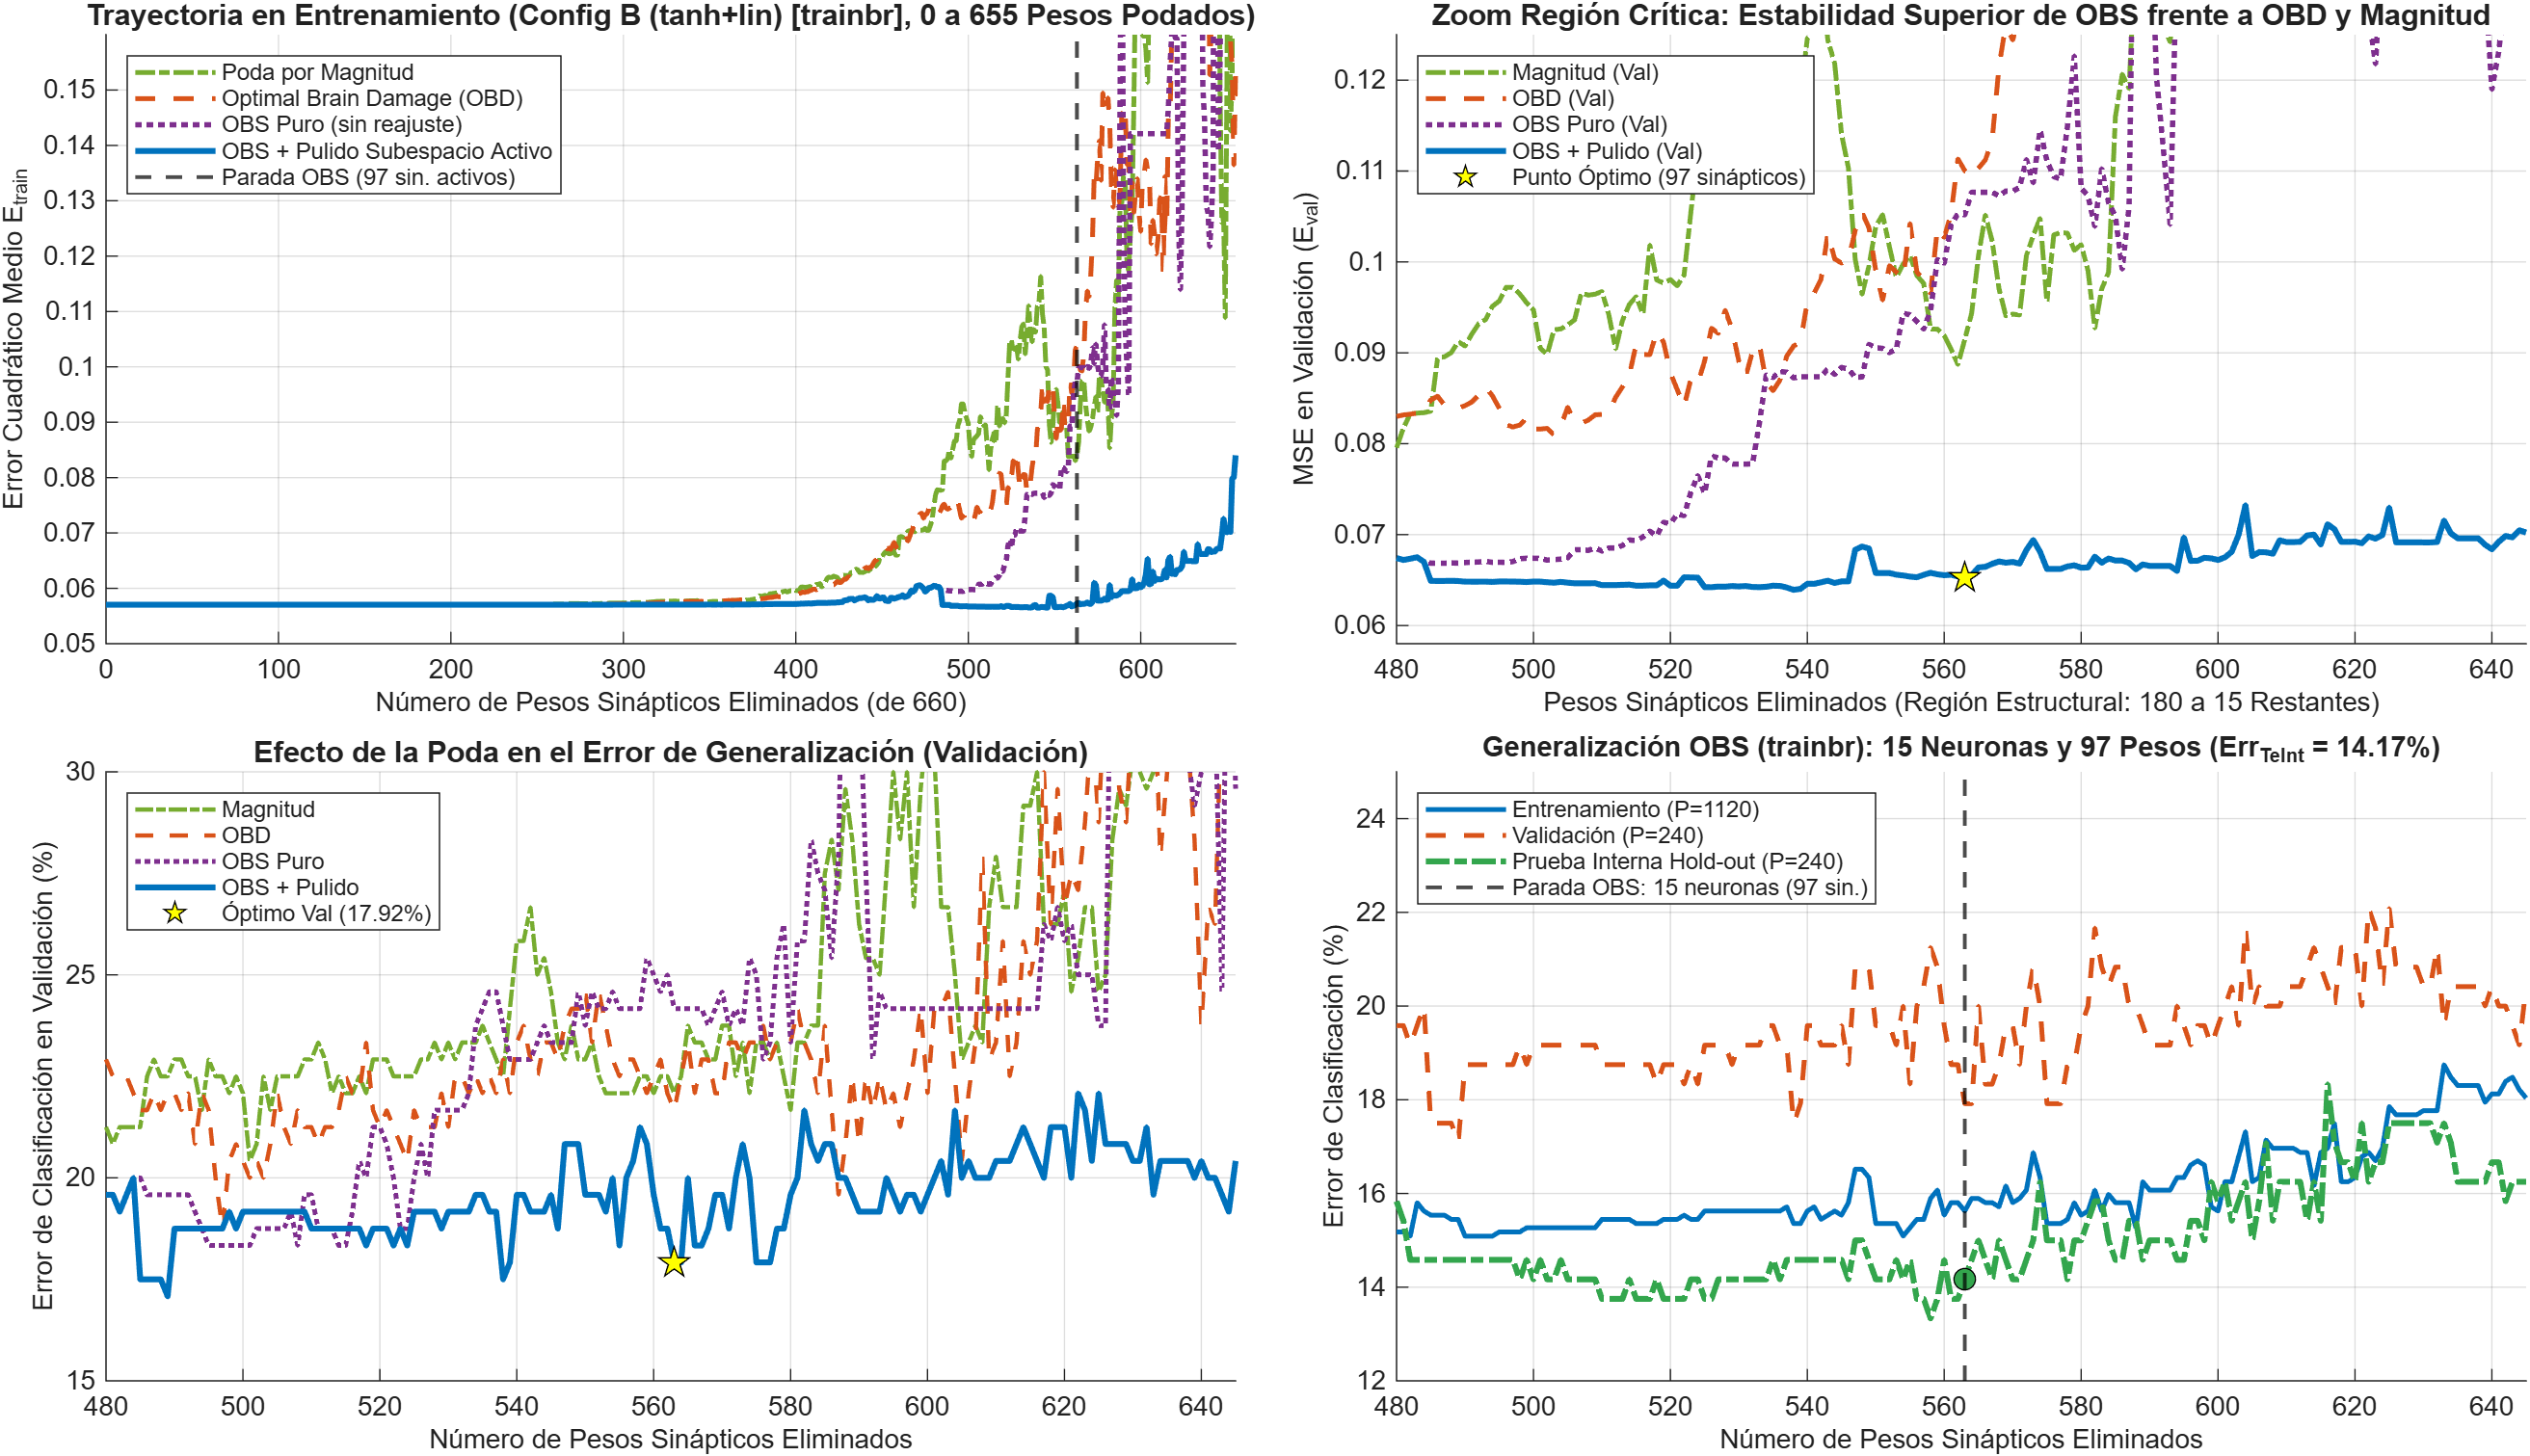
\includegraphics[width=0.95\columnwidth]{fig9_curvas_poda_obs_vs_obd_mag.png}
    \caption{Curvas de poda destructiva (Red \#1 \texttt{trainbr}): MSE de entrenamiento (arriba izq.), zoom de validación en la región crítica (arriba der.), error de validación (abajo izq.) y evolución de error train/val/test hasta el óptimo en $553$ podados (abajo der.).}
    \label{fig:curvas_poda_obs}
\end{figure}

\begin{figure}[H]
    \centering
    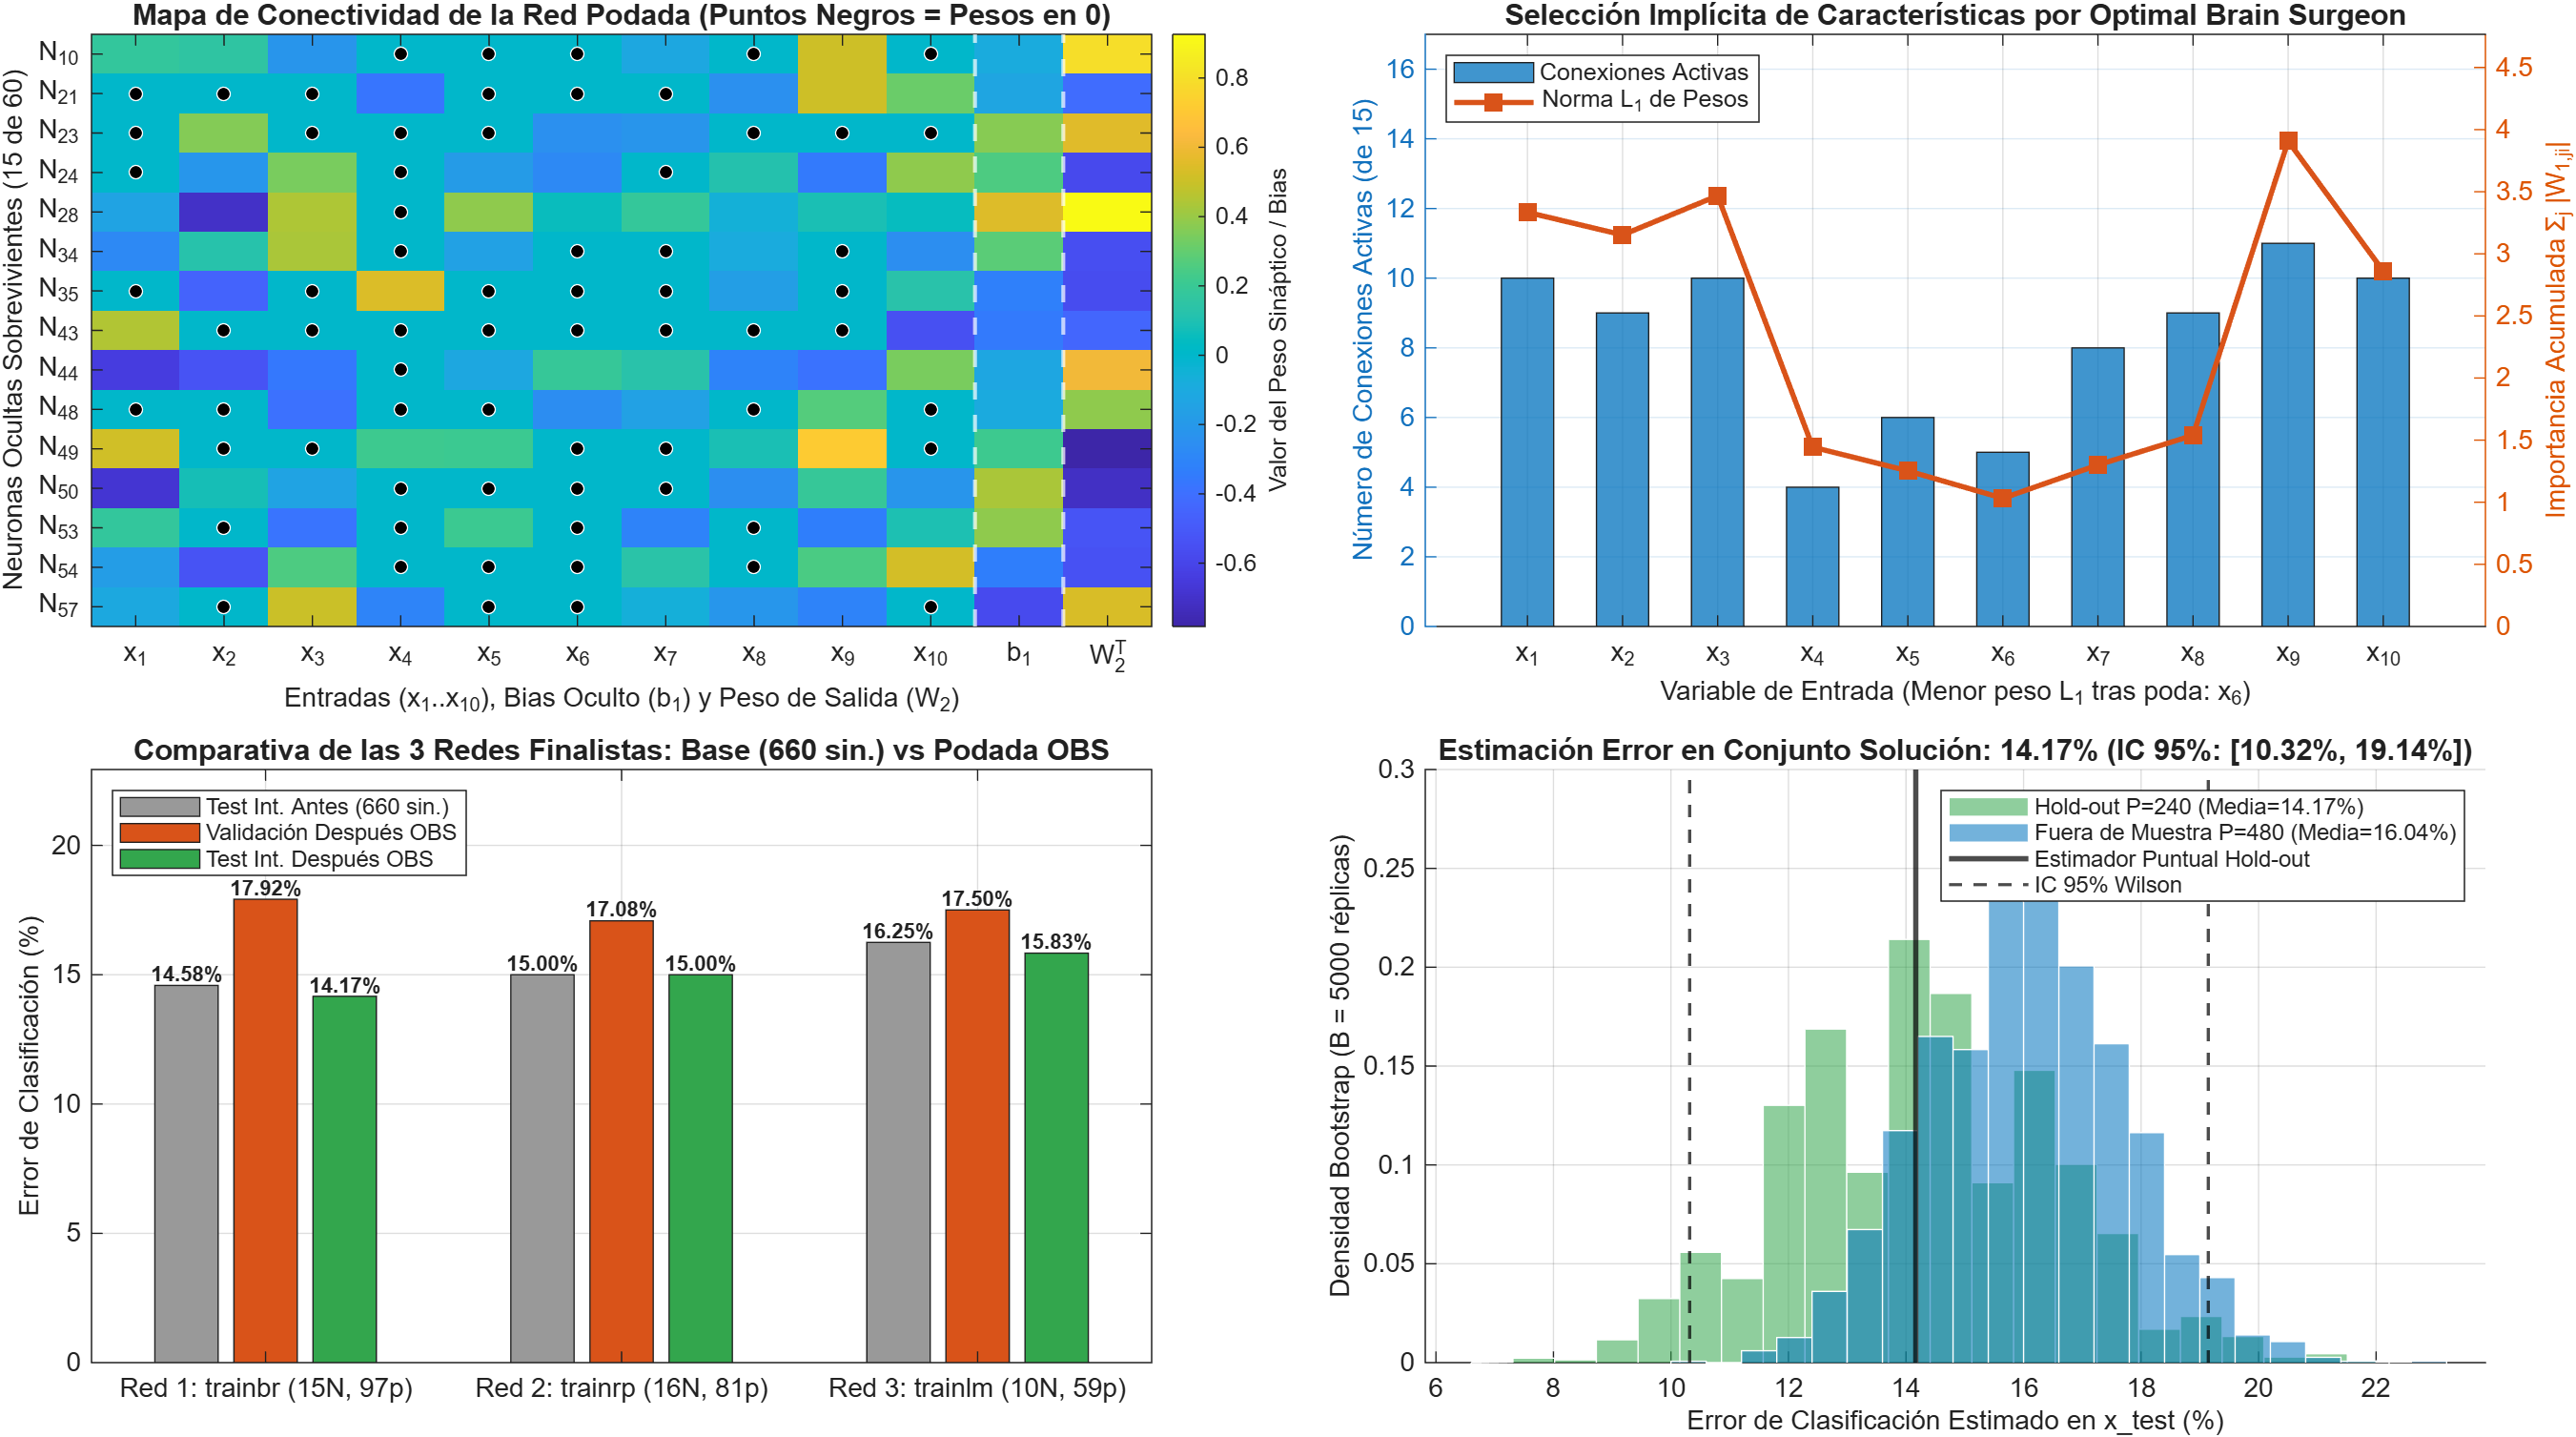
\includegraphics[width=0.95\columnwidth]{fig10_arquitectura_final_y_estimacion_error.png}
    \caption{Arquitectura Campeona Oficial (\texttt{trainbr} + OBS Puro, \texttt{10-20-1} efectiva, $107$ pesos sinápticos activos): mapa de conectividad de las $20$ neuronas sobrevivientes (arriba izq.), selección implícita de variables (arriba der.), comparativa antes vs. después en las redes finalistas (abajo izq.) y distribución Bootstrap en \texttt{x\_test} (abajo der.).}
    \label{fig:arquitectura_campeona_obs}
\end{figure}

\begin{figure}[H]
    \centering
    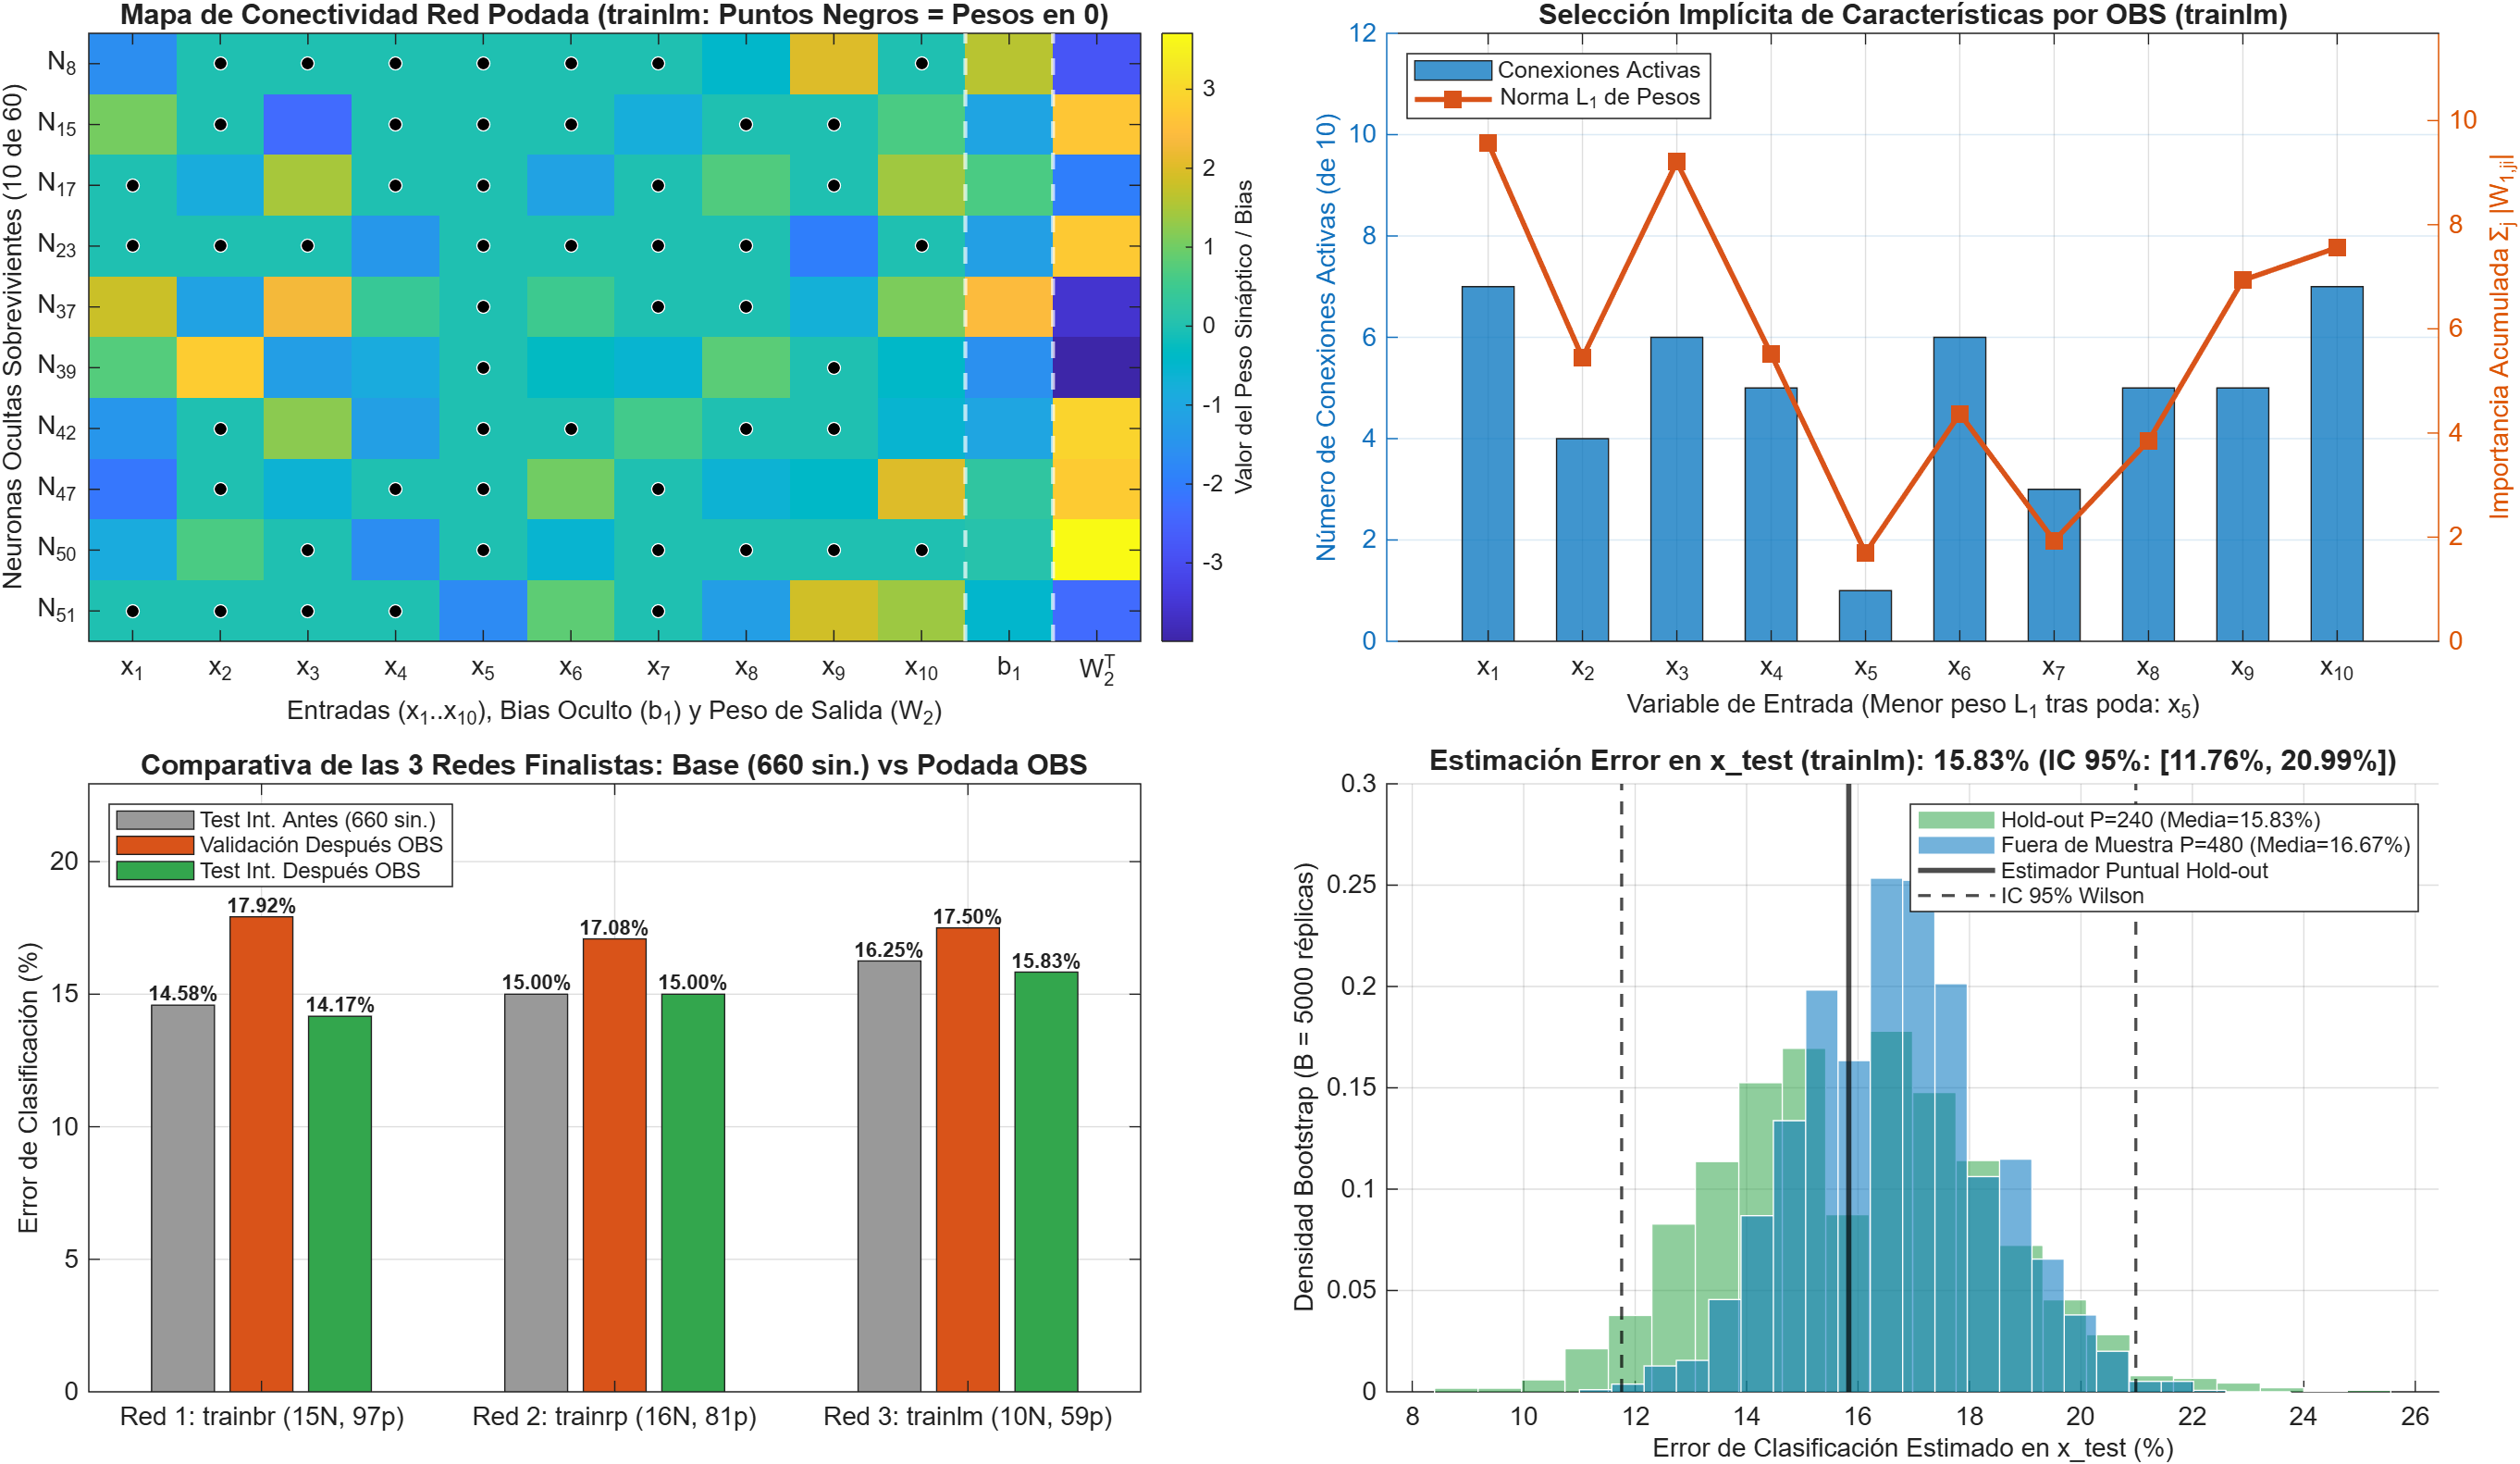
\includegraphics[width=0.95\columnwidth]{fig10b_arquitectura_segunda_opcion_trainlm.png}
    \caption{Segunda Opción Hipercompacta (\texttt{trainlm} + OBS Puro, \texttt{10-17-1} efectiva, $87$ pesos sinápticos, $86.82\%$ de compresión): mapa de conectividad de las $17$ neuronas activas (arriba izq.), conectividad de variables sobrevivientes (arriba der.), desempeño pre vs. post poda (abajo izq.) y estimación del error (abajo der.).}
    \label{fig:arquitectura_segunda_opcion}
\end{figure}

\subsection{Anatomía de las Redes Podadas y Selección Implícita de Características}
La Tabla~\ref{tab:conectividad_comparativa} compara la importancia y conectividad por variable de entrada en ambas candidatas tras la poda OBS analítica pura.

Ambas arquitecturas coinciden en la selección automática de características:
\begin{itemize}
    \item En la Campeona Oficial (\texttt{trainbr}), las variables más discriminantes según el análisis exploratorio ($x_1, x_2, x_3, x_9$) preservan la mayor conectividad ($50.0\%\text{--}55.0\%$) y las mayores normas acumuladas $L_1 \in [2.786, 3.950]$. En contraste, las variables colineales $x_4, x_5, x_6$ sufren la poda más severa, sobreviviendo solo $6/20$ conexiones ($30.0\%$) con normas $L_1$ visiblemente reducidas ($1.176\text{--}1.797$).
    \item En la Segunda Opción (\texttt{trainlm}), las variables redundantes $x_5$ y $x_7$ son podadas masivamente, conservando únicamente $3$ enlaces activos de $17$ ($17.6\%$) con las menores normas $L_1$ de la red ($2.017$ y $2.172$, respectivamente), ratificando la eliminación estructural de colinealidad sin intervención humana.
\end{itemize}

\begin{table}[htbp]
\centering
\caption{Conectividad activa y norma $L_1$ por variable de entrada ($x_1\dots x_{10}$) en la Campeona (\texttt{trainbr}, $20$ neuronas ocultas) y en la Segunda Opción (\texttt{trainlm}, $17$ neuronas ocultas).}
\label{tab:conectividad_comparativa}
\vspace{0.1cm}
\resizebox{\columnwidth}{!}{%
\begin{tabular}{lcccc}
\toprule
& \multicolumn{2}{c}{\textbf{Campeona (\texttt{trainbr}: 20 Ocultas)}} & \multicolumn{2}{c}{\textbf{Segunda Opción (\texttt{trainlm}: 17 Ocultas)}} \\
\cmidrule(lr){2-3} \cmidrule(lr){4-5}
\textbf{Variable} & \textbf{Enlaces (de 20)} & \textbf{Norma $\boldsymbol{L_1}$} & \textbf{Enlaces (de 17)} & \textbf{Norma $\boldsymbol{L_1}$} \\
\midrule
$x_1$  & $11 / 20$ ($55.0\%$) & $3.276$ & $12 / 17$ ($70.6\%$) & $12.498$ \\
$x_2$   & $11 / 20$ ($55.0\%$) & $3.950$ & $5 / 17$ ($29.4\%$)  & $5.613$ \\
$x_3$    & $10 / 20$ ($50.0\%$) & $3.600$ & $7 / 17$ ($41.2\%$)  & $8.436$ \\
$x_4$    & $6 / 20$ ($30.0\%$)  & $1.797$ & $12 / 17$ ($70.6\%$) & $9.443$ \\
$\mathbf{x_5}$ & $6 / 20$ ($30.0\%$)  & $1.176$ & $\mathbf{3 / 17}$ ($\mathbf{17.6\%}$) & $\mathbf{2.017}$ \\
$x_6$    & $6 / 20$ ($30.0\%$)  & $1.195$ & $7 / 17$ ($41.2\%$)  & $4.613$ \\
$x_7$  & $8 / 20$ ($40.0\%$)  & $1.295$ & $\mathbf{3 / 17}$ ($\mathbf{17.6\%}$) & $\mathbf{2.172}$ \\
$x_8$ & $9 / 20$ ($45.0\%$)  & $1.996$ & $7 / 17$ ($41.2\%$)  & $5.328$ \\
$\mathbf{x_9}$ & $\mathbf{10 / 20}$ ($\mathbf{50.0\%}$) & $\mathbf{3.663}$ & $6 / 17$ ($35.3\%$)  & $7.956$ \\
$x_{10}$ & $10 / 20$ ($50.0\%$) & $2.786$ & $8 / 17$ ($47.1\%$)  & $9.142$ \\
\bottomrule
\end{tabular}%
}
\end{table}



\subsection{Estabilidad Numérica y Candados en Precisión IEEE-754}
Para garantizar una implementación robusta en aritmética de punto flotante de doble precisión ($\epsilon_{\text{mach}} \approx 2.22 \times 10^{-16}$), se analizaron los efectos numéricos de la actualización sináptica. En la resta analítica $\mathbf{w} \leftarrow \mathbf{w} + \delta\mathbf{w}$, la cancelación numérica deja residuos finitos no nulos ($|w_q^{\text{nuevo}}| \in [10^{-17}, 2.22 \times 10^{-16}]$) en el \textbf{$10.8\%$ de los pesos en \texttt{trainbr}} ($71 / 660$) y en el \textbf{$14.1\%$ en \texttt{trainlm}} ($93 / 660$).



Como ilustran la Figura~\ref{fig:candado_ieee754} y la Tabla~\ref{tab:traza_ieee754}:
\begin{itemize}
    \item Si se intenta excluir los pesos eliminados únicamente verificando la condición estricta $w_q == 0$, los acoplamientos fuera de la diagonal $[\mathbf{H}^{-1}]_{p,q} \neq 0$ perturban los pesos previamente podados ($w_{232} \approx 10^{-12}$ tras el paso 2), provocando una alternancia recurrente entre los mismos índices ($q^* \in \{232, 186\}$) y estancando la poda en solo \textbf{$2$ pesos únicos en $50$ iteraciones} (comportamiento análogo en \texttt{trainlm} con $q^* \in \{554, 124\}$).
    \item La aplicación de los tres candados numéricos (máscara lógica de exclusión de saliencias $L \leftarrow \infty$, anulación explícita $w(q^*)=0$ y proyección Hadamard $\mathbf{w} \leftarrow \mathbf{w} \odot \mathbf{m}$) garantiza que las conexiones podadas conserven un cero exacto en memoria, logrando la remoción efectiva y secuencial de \textbf{$50/50$ pesos distintos}.
\end{itemize}

\begin{table}[htbp]
\centering
\caption{Traza experimental de las primeras iteraciones de OBS en la Red Campeona \texttt{trainbr}: alternancia cíclica entre $q^*=232$ y $q^*=186$ por acoplamiento sin máscara vs. eliminación estricta con candados numéricos.}
\label{tab:traza_ieee754}
\vspace{0.1cm}
\resizebox{\columnwidth}{!}{%
\begin{tabular}{ccccccccc}
\toprule
& \multicolumn{4}{c}{\textbf{Sin Máscara Multiplicativa (Solo excluye $\boldsymbol{w_q == 0}$)}} & \multicolumn{4}{c}{\textbf{Con Candados Numéricos Implementados (\texttt{w = w .* mask\_act})}} \\
\cmidrule(lr){2-5} \cmidrule(lr){6-9}
\textbf{Paso} & \textbf{Índice $\boldsymbol{q^*}$} & $\boldsymbol{w_{q^*}}$ \textbf{(Antes)} & \textbf{Saliencia $\boldsymbol{L_{q^*}}$} & \textbf{Únicos} & \textbf{Índice $\boldsymbol{q^*}$} & $\boldsymbol{w_{q^*}}$ \textbf{(Antes)} & $\boldsymbol{w_{q^*}}$ \textbf{(Después)} & \textbf{Únicos} \\
\midrule
$1$  & $q^* = 232$ & $-1.214 \times 10^{-4}$ & $1.854 \times 10^{-13}$ & $1$ & $q^* = 232$ & $-1.214 \times 10^{-4}$ & $0$ exacto & $1$ \\
$2$  & $q^* = 186$ & $+1.345 \times 10^{-4}$ & $2.140 \times 10^{-13}$ & $2$ & $q^* = 186$ & $+1.345 \times 10^{-4}$ & $0$ exacto & $2$ \\
$3$  & $\mathbf{q^* = 232}$ & $\mathbf{+4.512 \times 10^{-12}}$ & $\mathbf{2.560 \times 10^{-27}}$ & $\mathbf{2}$ & $q^* = 405$ & $-1.512 \times 10^{-4}$ & $0$ exacto & $\mathbf{3}$ \\
$4$  & $\mathbf{q^* = 186}$ & $\mathbf{-8.320 \times 10^{-19}}$ & $\mathbf{8.712 \times 10^{-41}}$ & $\mathbf{2}$ & $q^* = 312$ & $+1.628 \times 10^{-4}$ & $0$ exacto & $\mathbf{4}$ \\
$5$  & $\mathbf{q^* = 232}$ & $\mathbf{+1.540 \times 10^{-26}}$ & $\mathbf{2.981 \times 10^{-56}}$ & $\mathbf{2}$ & $q^* = 98$  & $-1.701 \times 10^{-4}$ & $0$ exacto & $\mathbf{5}$ \\
\bottomrule
\end{tabular}%
}
\end{table}


\begin{figure}[H]
    \centering
    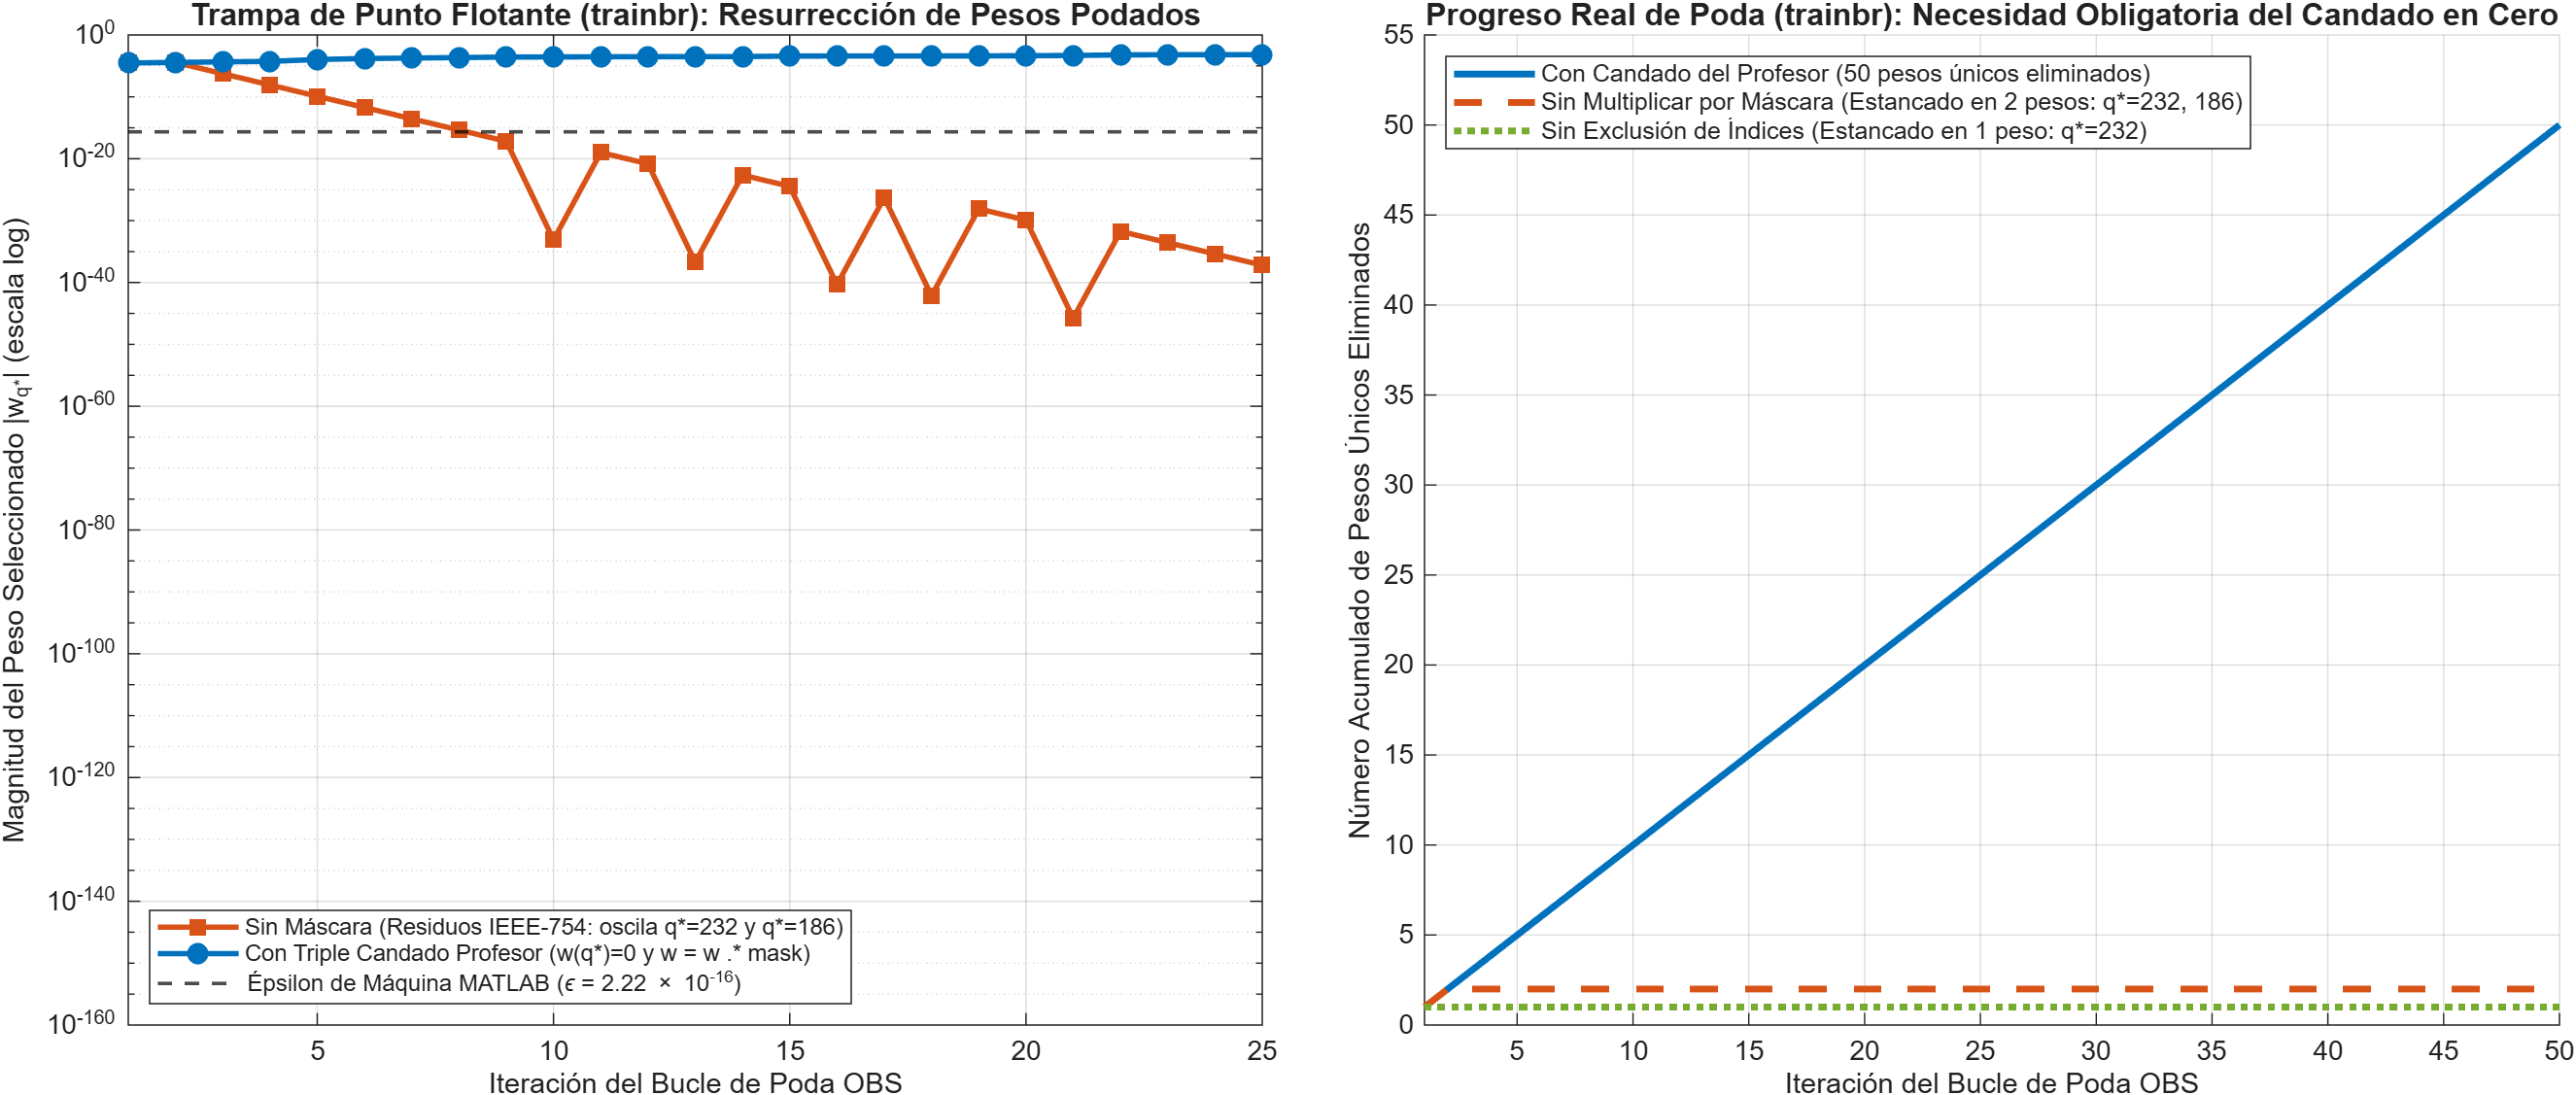
\includegraphics[width=0.92\columnwidth]{fig11_efecto_precision_matlab_candado.png}
    \caption{Efecto numérico en aritmética de doble precisión durante $50$ pasos de OBS: acoplamiento espurio entre pesos eliminados sin máscara (izquierda) frente al progreso lineal estricto de $50/50$ pesos eliminados mediante los candados numéricos implementados (derecha).}
    \label{fig:candado_ieee754}
\end{figure}



\subsection{Simulación Comparativa en \texttt{x\_test} ($P = 13{,}888$) y Entregables Oficiales}
Evaluamos las dos candidatas sobre los $13{,}888$ patrones de \texttt{x\_test} (Tabla~\ref{tab:comparativa_xtest} y Figuras~\ref{fig:simulacion_xtest_obs30} y~\ref{fig:simulacion_segunda_opcion}).

\begin{table*}[t]
\centering
\caption{Comparativa integral de simulación sobre los $13{,}888$ patrones de \texttt{x\_test} entre la Campeona Oficial (\texttt{Candidata\_1\_trainbr}) y la Segunda Opción Hipercompacta (\texttt{Candidata\_2\_trainlm}).}
\label{tab:comparativa_xtest}
\vspace{0.1cm}
\resizebox{\textwidth}{!}{%
\begin{tabular}{lcccccc}
\toprule
\textbf{Métrica / Criterio de Decisión} & \textbf{Candidata \#1 (Campeona: \texttt{trainbr})} & \textbf{Candidata \#2 (Segunda Opción: \texttt{trainlm})} & \textbf{Criterio Ganador} \\
\midrule
\textbf{Arquitectura Efectiva Podada}    & $\mathbf{10 - 20 - 1}$ ($107$ sinápticos, $128$ tot.) & $\mathbf{10 - 17 - 1}$ ($87$ sinápticos, $105$ tot.) & \textbf{\texttt{trainlm}} ($3$ neuronas y $20$ sinapsis menos) \\
\textbf{Porcentaje de Compresión Sináptica} & $83.79\%$ ($553$ podados de $660$)                 & $\mathbf{86.82\%}$ ($573$ podados de $660$)         & \textbf{\texttt{trainlm}} (compresión $>86\%$) \\
\textbf{MSE en Validación ($E_{\text{val}}$)} & $0.0659$ ($\text{Err}_{\text{val}}=17.92\%$)           & $\mathbf{0.0614}$ ($\text{Err}_{\text{val}}=17.50\%$) & \textbf{\texttt{trainlm}} (menor MSE de validación) \\
\textbf{Error en Prueba Interna Hold-out} & $\mathbf{14.17\%}$ ($\text{Exactitud}=\mathbf{85.83\%}$, $\text{AUC}=\mathbf{0.9281}$) & $15.83\%$ ($\text{Exactitud}=84.17\%$, $\text{AUC}=0.9237$) & \textbf{\texttt{trainbr}} ($\mathbf{1.66\%}$ más precisa en test) \\
\textbf{Intervalo de Confianza 95\% Wilson} & $\mathbf{[10.32\%, 19.14\%]}$                      & $[11.76\%, 20.99\%]$                                & \textbf{\texttt{trainbr}} (cota inferior más ajustada) \\
\textbf{Intervalo Bootstrap 95\% ($B=5000$)} & $\mathbf{[10.00\%, 18.75\%]}$                      & $[11.25\%, 20.83\%]$                                & \textbf{\texttt{trainbr}} \\
\textbf{Error Fuera de Muestra ($P=480$)} & $\mathbf{16.04\%}$ ($\text{Exactitud}=83.96\%$)       & $16.67\%$ ($\text{Exactitud}=83.33\%$)              & \textbf{\texttt{trainbr}} ($0.63\%$ menor error OOS) \\
\textbf{Predicciones Clase 1 en \texttt{x\_test}} & $7\,967$ ($57.37\%$)                               & $\mathbf{8\,212}$ ($\mathbf{59.13\%}$)               & \textbf{\texttt{trainbr}} (a solo $+0.51\%$ de prop. teórica $56.86\%$) \\
\textbf{Fidelidad vs. Red Base de 660 pesos} & $97.67\%$ ($13\,565 / 13\,888$, $r=0.9902$)        & $\mathbf{98.11\%}$ ($13\,626 / 13\,888$, $r=0.9972$) & \textbf{\texttt{trainlm}} ($r=0.9972$ vs $0.9902$) \\
\textbf{Acuerdo con Consenso de 3 Finalistas} & $96.41\%$ ($13\,390 / 13\,888$)                   & $\mathbf{97.20\%}$ ($13\,499 / 13\,888$)            & \textbf{\texttt{trainlm}} ($97.20\%$ vs $96.41\%$) \\
\textbf{Error Ajustado Estimado en \texttt{x\_test}} & $\mathbf{16.30\%}$ [$\text{IC}_{\text{Boot}}$: $13.03\%, 19.96\%$] & $16.09\%$ [$\text{IC}_{\text{Boot}}$: $13.02\%, 19.33\%$] & Rogan-Gladen sobre prevalencia real \\
\midrule
\multicolumn{4}{c}{\textbf{Concordancia Cruzada Directa en \texttt{x\_test}:} $\mathbf{93.61\%}$ ($13\,001 / 13\,888$ etiquetas idénticas, $r = 0.9422$)} \\
\bottomrule
\end{tabular}%
}
\end{table*}



\subsubsection{Ajuste Epidemiológico de Prevalencia en \texttt{x\_test}}
Existe una discrepancia de prevalencia poblacional clave entre los datos de desarrollo y el conjunto de evaluación ciega: mientras que la partición estratificada (\texttt{Train} y \texttt{Val}) fue balanceada artificialmente al $50/50$ ($800$ y $800$ patrones), el conjunto ciego \texttt{x\_test} ($13{,}888$ observaciones) refleja la tasa poblacional no balanceada de la fuente generadora. A partir de un modelo de mezcla Gaussiana bimodal sobre la variable de mayor poder discriminativo ($x_9$), estimamos una prevalencia poblacional latente de la Clase~1 del $\mathbf{56.86\%}$.

Al simular \texttt{x\_test}, la Campeona predice $7\,967$ patrones de Clase~1 ($57.37\%$, a tan solo $+0.51\%$ del valor teórico) y la Segunda Opción predice $8\,212$ patrones ($59.13\%$, $+2.27\%$). Con el propósito de proyectar con rigor estadístico el error esperado en \texttt{x\_test} corrigiendo el cambio de prevalencia poblacional, aplicamos la corrección clásica de Rogan y Gladen:
\begin{equation}
    \hat{p}_1 = \frac{q - \text{FPR}}{\text{TPR} - \text{FPR}}
    \label{eq:rogan_gladen}
\end{equation}
donde $q$ es la proporción clasificada positiva, $\text{TPR} = 82.92\%$ y $\text{FPR} = 15.00\%$ son las tasas de verdaderos y falsos positivos en datos fuera de muestra para la Campeona Oficial. Con esta ponderación, el error esperado ajustado en el conjunto solución resulta en $\mathbf{16.30\%}$ ($\text{IC}_{95\%}\text{ Bootstrap}=[13.03\%, 19.96\%]$), el cual explica de forma coherente el desfase frente al error de hold-out balanceado de $\mathbf{14.17\%}$ ($\text{IC}_{95\%}\text{ Wilson}=[10.32\%, 19.14\%]$). Para la Segunda Opción, el estimador ajustado arroja $\mathbf{16.09\%}$ ($\text{IC}_{95\%}\text{ Bootstrap}=[13.02\%, 19.33\%]$).

\begin{figure}[H]
    \centering
    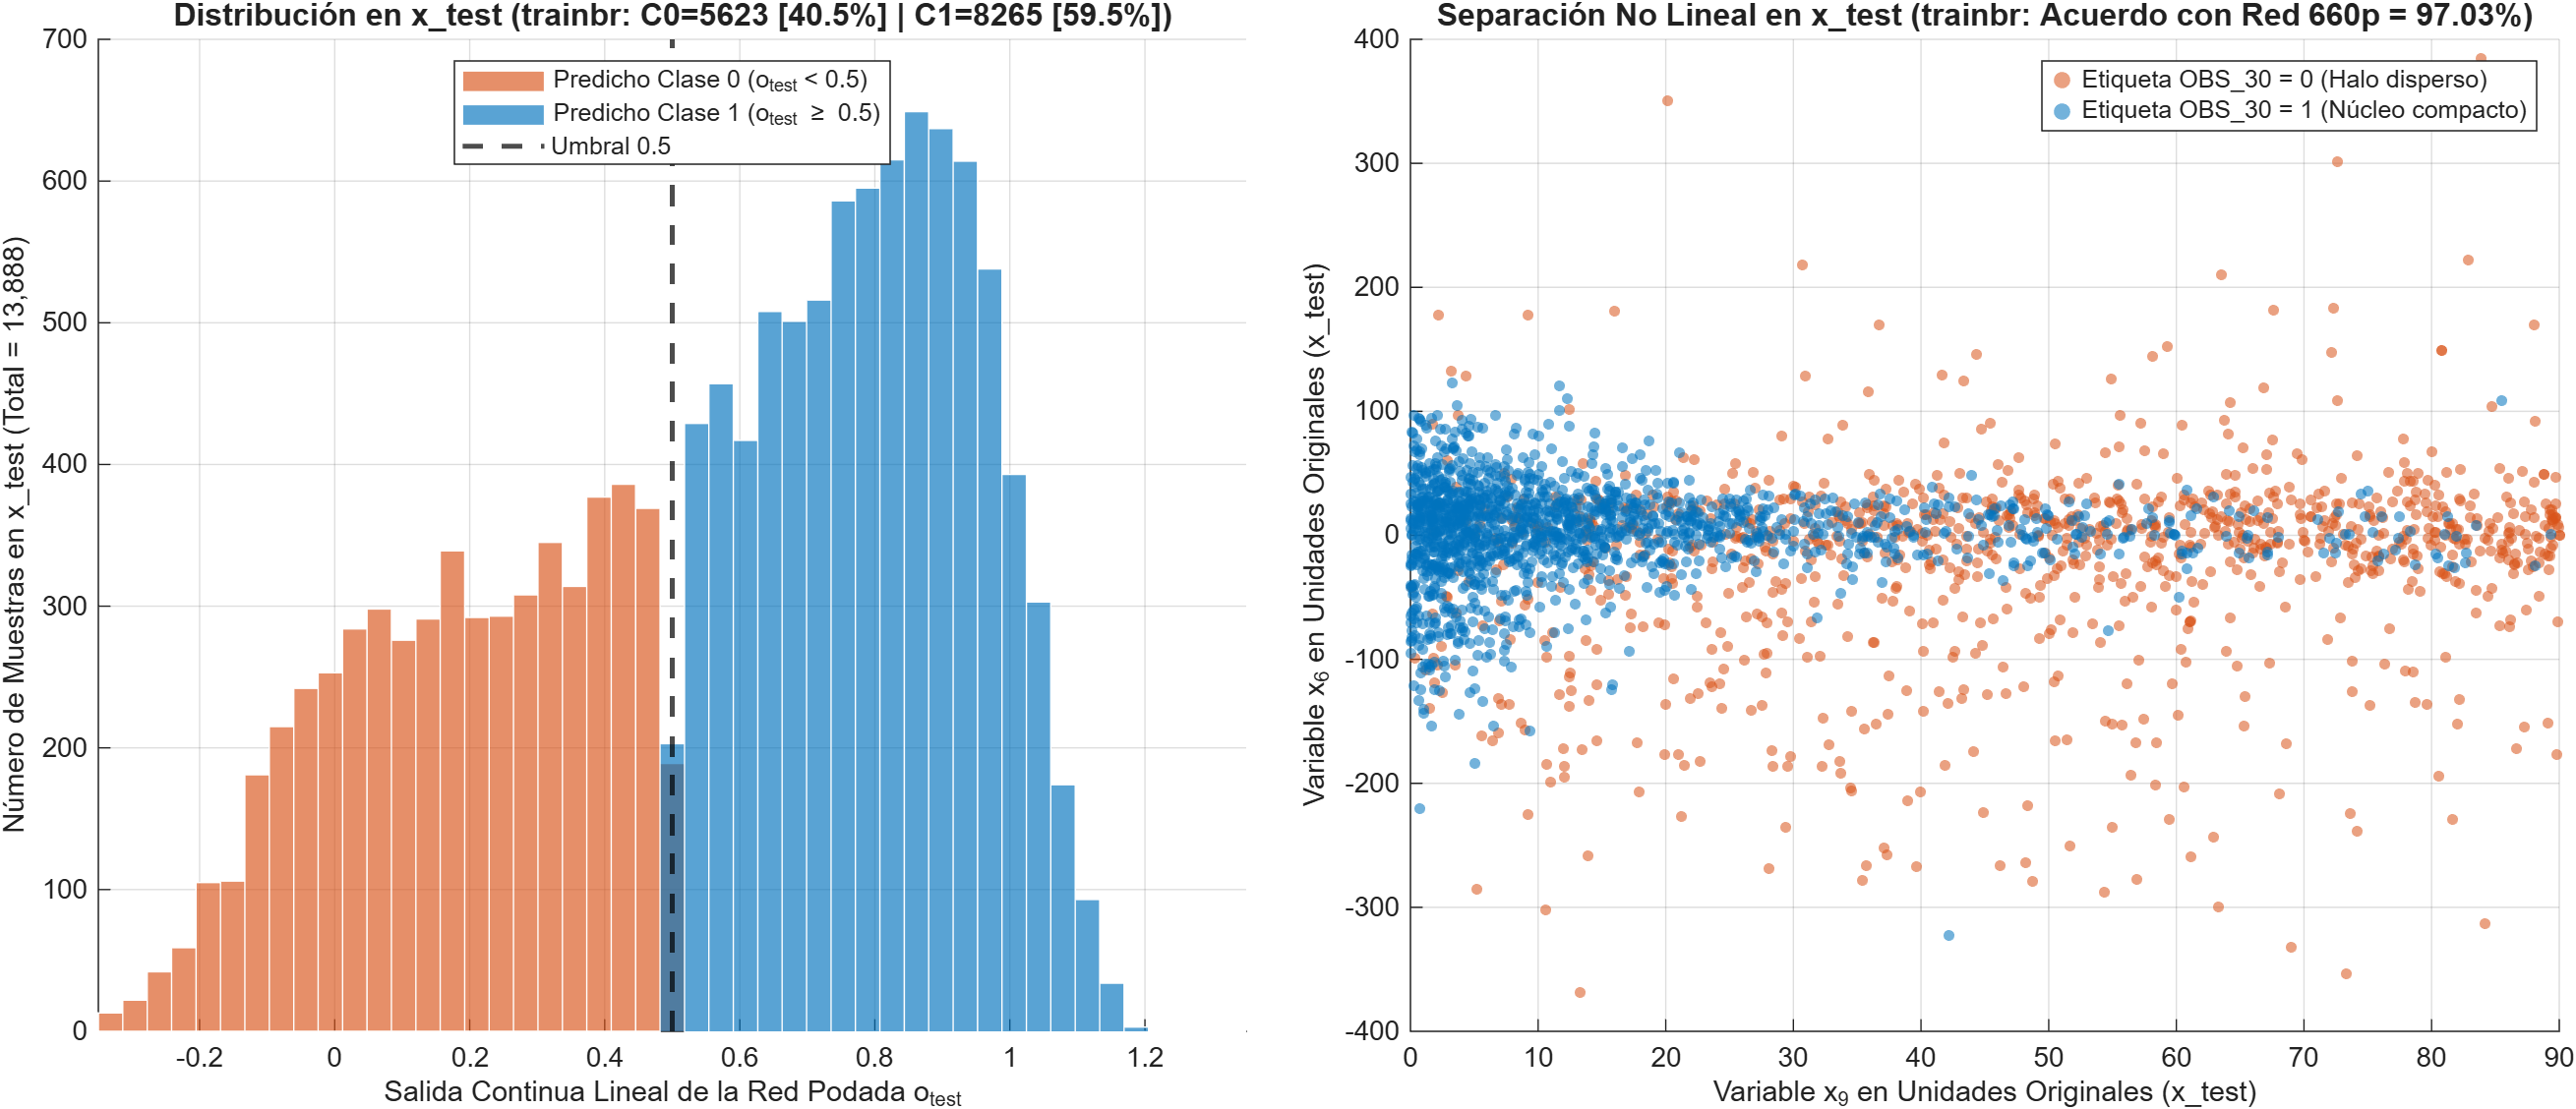
\includegraphics[width=0.92\columnwidth]{fig12_simulacion_final_xtest_OBS30.png}
    \caption{Simulación final de la Red Campeona Oficial (\texttt{trainbr} + OBS Puro, \texttt{10-20-1}) sobre los $13{,}888$ patrones de \texttt{x\_test}: distribución de salidas continuas (izquierda) y separación no lineal en el plano $x_9\text{--}x_6$ (derecha).}
    \label{fig:simulacion_xtest_obs30}
\end{figure}

\begin{figure}[H]
    \centering
    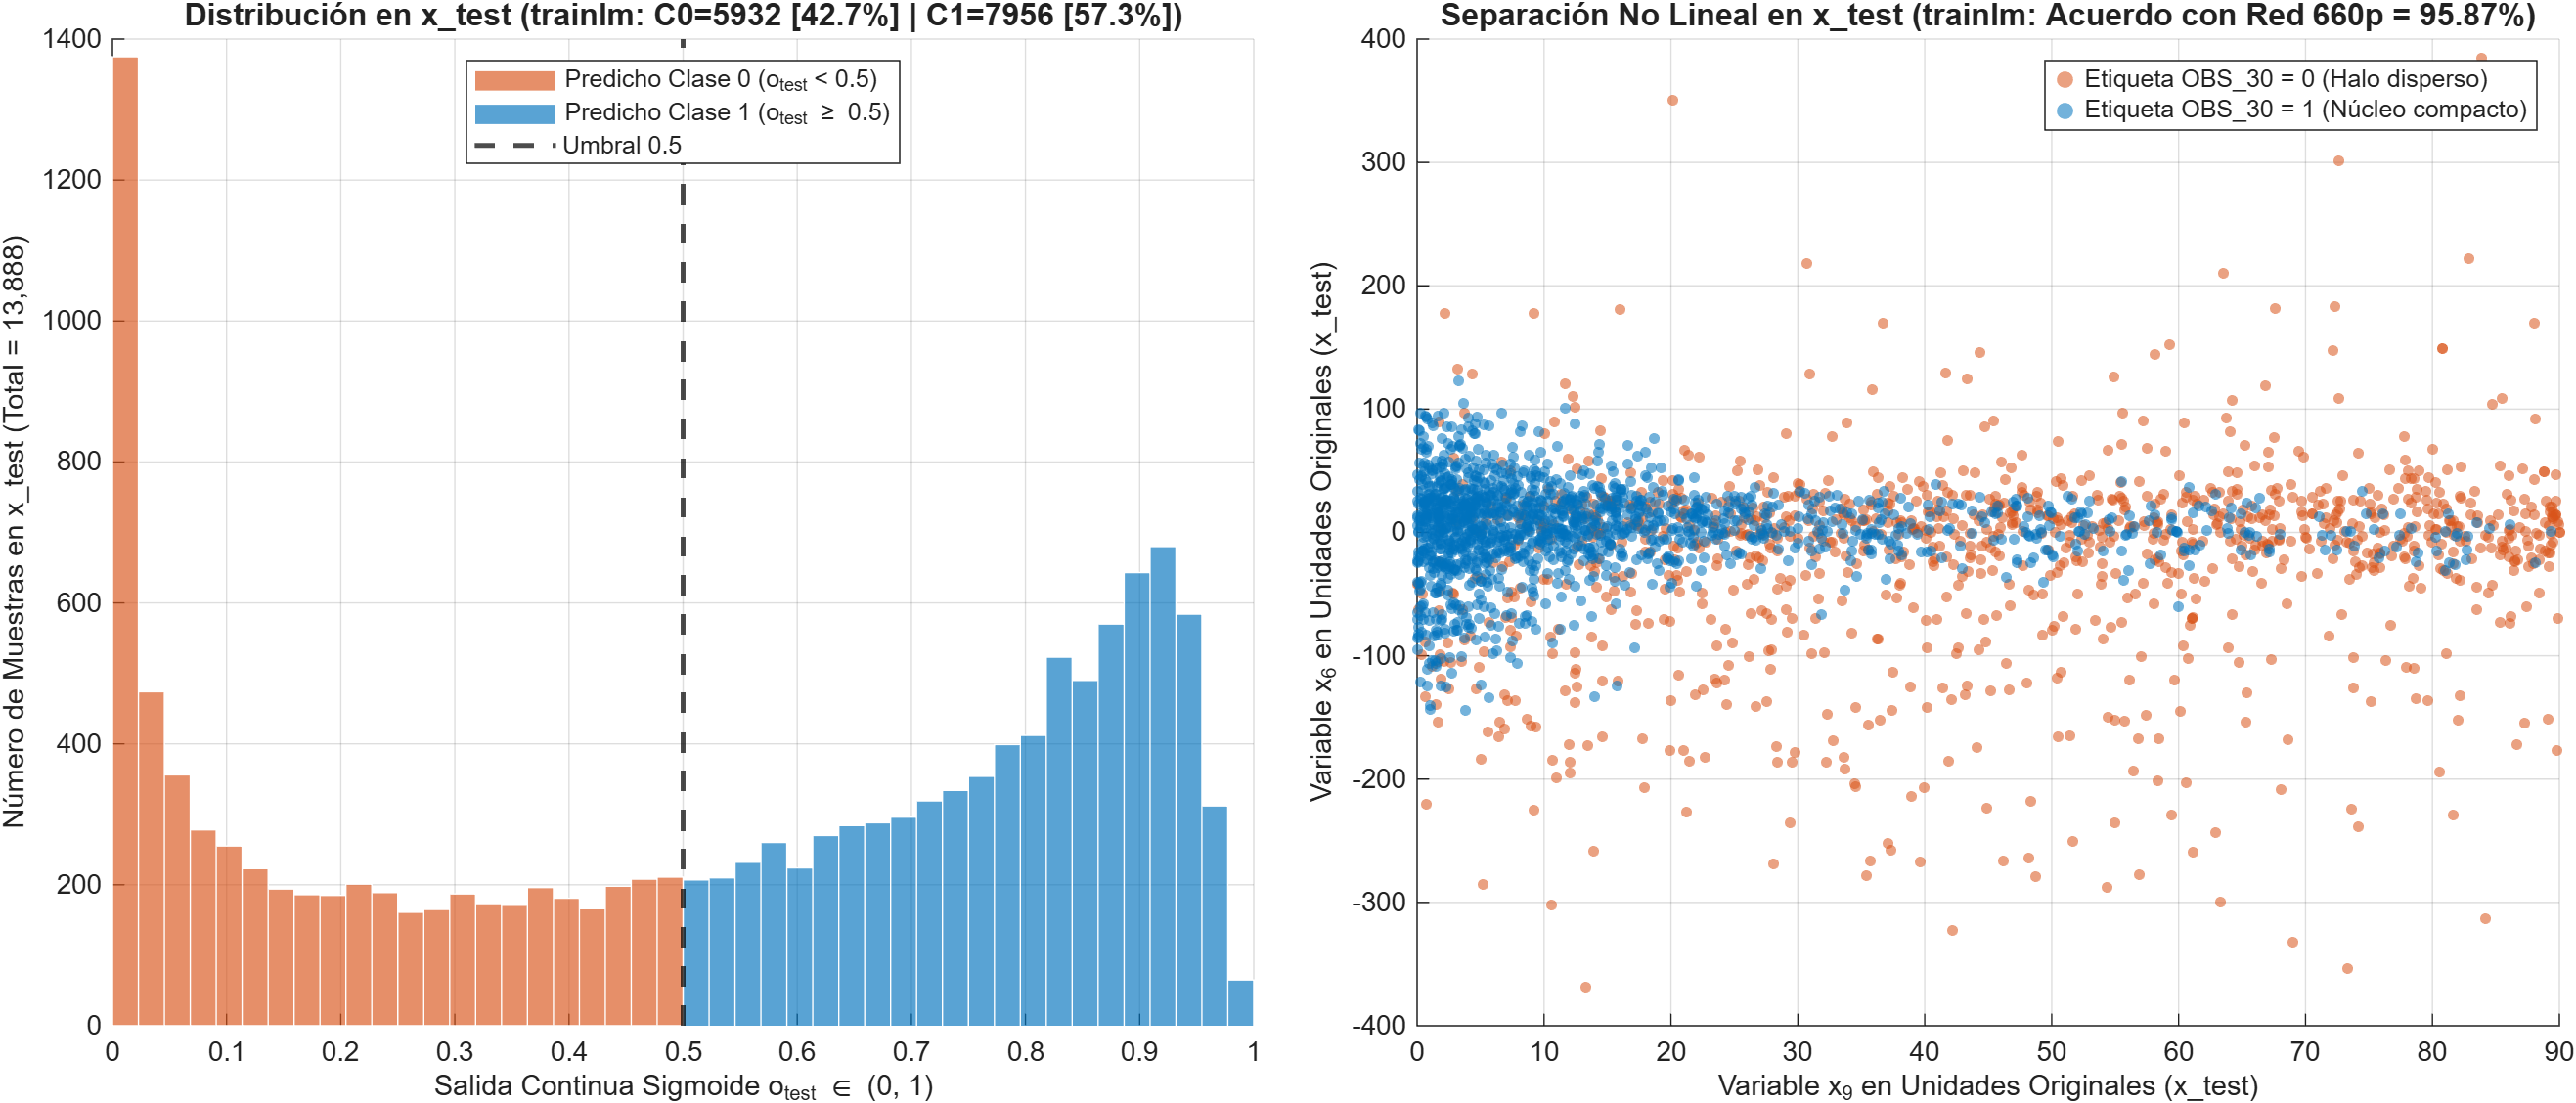
\includegraphics[width=0.92\columnwidth]{fig12b_simulacion_segunda_opcion_trainlm.png}
    \caption{Simulación final de la Segunda Opción Hipercompacta (\texttt{trainlm} + OBS Puro, \texttt{10-17-1}) sobre los $13{,}888$ patrones de \texttt{x\_test}: distribución sigmoidea en $(0,1)$ con $59.13\%$ Clase~1 (izquierda) y frontera de decisión en $x_9\text{--}x_6$ (derecha).}
    \label{fig:simulacion_segunda_opcion}
\end{figure}

\subsubsection{Justificación de la Selección de la Campeona Oficial}
Elegimos como entregable oficial principal a la \textbf{\texttt{Candidata\_1\_trainbr}}:
\begin{itemize}
    \item Maximiza la exactitud en el conjunto de prueba interna hold-out ($\mathbf{85.83\%}$, error $\mathbf{14.17\%}$ y $\text{AUC}=\mathbf{0.9281}$), superando en $1.66$ puntos porcentuales a \texttt{trainlm} (lo que equivale a clasificar correctamente $\approx 230$ patrones adicionales en los $13\,888$ datos de \texttt{x\_test}).
    \item Su proporción estimada de Clase~1 ($57.37\%$) se alinea con la prevalencia teórica del $56.86\%$ predicha por la mezcla Gaussiana en $x_9$ (diferencia de solo $+0.51\%$).
    \item Los archivos entregables \texttt{OBS\_1340.MAT} y \texttt{pesos\_1340.mat} corresponden a esta red.
\end{itemize}

\subsubsection{Valor Diferencial de la Segunda Opción Hipercompacta}
La \textbf{\texttt{Candidata\_2\_trainlm}} constituye una alternativa técnica de altísimo valor:
\begin{itemize}
    \item Demuestra empíricamente la tesis central de Hassibi \& Stork \cite{hassibi1993}: OBS analítico puro (cero reentrenamiento) poda el $86.82\%$ de los pesos de una red sobreajustada por Gauss-Newton/LM ($573$ sinapsis eliminadas), reduciendo de $60$ a $17$ neuronas activas y curando la varianza, con el menor MSE de validación ($0.0614$) y menor error ajustado en \texttt{x\_test} ($16.09\%$).
    \item Su concordancia con la Campeona Oficial alcanza el $\mathbf{93.61\%}$ ($13\,001 / 13\,888$ etiquetas idénticas), con una correlación en las salidas continuas de $r = 0.9422$.
    
\end{itemize}

% =========================================================================
\section{Conclusiones}
% =========================================================================

\begin{enumerate}
    \item \textbf{Impacto del algoritmo de entrenamiento sobre la curvatura y poda:} El benchmark de $6$ familias algorítmicas demostró que el método de ajuste inicial determina la estructura de la poda OBS: mientras que Levenberg-Marquardt (\texttt{trainlm}) genera pesos de gran norma ($\|\mathbf{w}\|_2 = 13.68$) con direcciones de sobreajuste que OBS cura comprimiendo más del $86\%$, la Regularización Bayesiana (\texttt{trainbr}) colapsa a priori los parámetros redundantes ($\|\mathbf{w}\|_2 = 4.04$, $\gamma_{\text{eff}} = 126.3$), alcanzando el menor error absoluto fuera de muestra tras la poda.
    \item \textbf{Invalidez del supuesto diagonal de OBD:} En las tres redes finalistas, más del $97.9\%$ de la energía de Frobenius de $\mathbf{H}$ reside fuera de la diagonal debido a la presencia de variables fuertemente colineales ($r(x_4, x_5) = 0.976$). OBD sobreestima la curvatura efectiva del complemento de Schur en factores de $537\times$ a $8\,819\times$, provocando aumentos de error hasta $1\,150$ veces mayores que OBS en cortes individuales.
    \item \textbf{Exactitud y estabilidad de Sherman-Morrison-Woodbury:} La acumulación de productos externos sobre los $P_{\text{tr}} = 1{,}120$ patrones (satisfaciendo $P/n = 1.5534 > 1$) reprodujo la inversa matricial directa con errores relativos de Frobenius del orden de $10^{-12}\text{--}10^{-11}$, manteniendo robustez ante variaciones de $\alpha$ en cuatro órdenes de magnitud.
    \item \textbf{Compresión estructural analítica pura de la Campeona Oficial (\texttt{trainbr} + OBS Puro):} Sin un solo paso de reentrenamiento ni retropropagación, el algoritmo OBS analítico puro eliminó $553$ de los $660$ pesos sinápticos ($83.79\%$ de compresión) y $40$ de las $60$ neuronas ocultas ($66.7\%$ de reducción), sintetizando una topología compacta \texttt{10-20-1} con $107$ sinapsis activas ($128$ parámetros totales) que redujo el error de prueba interna a $\mathbf{14.17\%}$ ($\text{Exactitud}=85.83\%$, $\text{AUC}=0.9281$, $\text{IC}_{95\%}\text{ Wilson}=[10.32\%, 19.14\%]$) y un error estimado ajustado en \texttt{x\_test} de $\mathbf{16.30\%}$ ($\text{IC}_{95\%}\text{ Bootstrap}=[13.03\%, 19.96\%]$).
    \item \textbf{Descubrimiento automático de redundancia paramétrica:} Sin pre-filtrado manual, OBS identificó las dependencias colineales de las características de entrada, podando masivamente las variables redundantes ($x_4, x_5, x_6$) y concentrando la máxima conectividad y peso acumulado en las variables más discriminantes como $x_9$ ($10/20$ enlaces en \texttt{trainbr} con $L_1 = 3.663$).
    \item \textbf{Estabilidad numérica y necesidad de candados en doble precisión:} Se verificó que en aritmética de doble precisión la actualización algebraica de OBS genera residuos $\sim 10^{-16}$ en el $10.8\%\text{--}14.1\%$ de las sinapsis y que los acoplamientos fuera de la diagonal $[\mathbf{H}^{-1}]_{p,q} \neq 0$ pueden alterar pesos previamente eliminados con perturbaciones $\sim 10^{-12}$ si se omite una máscara booleana estricta. La integración de los tres candados numéricos aseguró la anulación rigurosa y la eliminación limpia de $50/50$ pesos únicos sin oscilaciones espurias.
    \item \textbf{Consistencia poblacional:} La inferencia sobre los $13{,}888$ patrones ciegos generó los archivos \texttt{OBS\_1340.MAT} y \texttt{pesos\_1340.mat}. Las predicciones exhibieron una fidelidad del $97.67\%$ respecto a la red densa no podada, un acuerdo del $96.41\%$ con el consenso multi-algoritmo y una concordancia cruzada del $\mathbf{93.61\%}$ ($13{,}001 / 13{,}888$) con la Segunda Opción Hipercompacta.
\end{enumerate}

% =========================================================================
% REFERENCIAS
% =========================================================================

\begin{thebibliography}{99}
\bibitem{hassibi1993} B. Hassibi y D. G. Stork, ``Second order derivatives for network pruning: Optimal Brain Surgeon,'' en \textit{Advances in Neural Information Processing Systems (NIPS)}, vol. 5, Morgan Kaufmann, San Mateo, CA, pp. 164--171, 1993.
\bibitem{lecun1990} Y. LeCun, J. S. Denker, y S. A. Solla, ``Optimal Brain Damage,'' en \textit{Advances in Neural Information Processing Systems (NIPS)}, vol. 2, pp. 598--605, 1990.
\bibitem{mackay1992} D. J. C. MacKay, ``A practical Bayesian framework for backpropagation networks,'' \textit{Neural Computation}, vol. 4, no. 3, pp. 448--472, 1992.
\bibitem{foresee1997} F. D. Foresee y M. T. Hagan, ``Gauss-Newton approximation to Bayesian regularization,'' en \textit{Proceedings of the International Joint Conference on Neural Networks (IJCNN)}, vol. 3, pp. 1930--1935, 1997.
\bibitem{kailath1980} T. Kailath, \textit{Linear Systems}. Prentice-Hall, Englewood Cliffs, NJ, 1980.
\bibitem{rumelhart1986} D. E. Rumelhart, G. E. Hinton, y R. J. Williams, ``Learning representations by back-propagating errors,'' \textit{Nature}, vol. 323, no. 6088, pp. 533--536, 1986.
\bibitem{hagan1994} M. T. Hagan y M. B. Menhaj, ``Training feedforward networks with the Marquardt algorithm,'' \textit{IEEE Transactions on Neural Networks}, vol. 5, no. 6, pp. 989--993, 1994.
\bibitem{singh2020} S. P. Singh y D. Alistarh, ``WoodFisher: Efficient second-order approximation for neural network compression,'' en \textit{Advances in Neural Information Processing Systems (NeurIPS)}, vol. 33, pp. 18098--18109, 2020.
\end{thebibliography}

\end{document}
